%generare il pdf con il comando: pdflatex main.tex
\documentclass[a4paper, oneside, openany, dvipsnames, table]{article}
\usepackage{../template/SWEightStyle}
\usepackage{tabularx}
\usepackage{ltablex}
\newcommand{\Titolo}{Manuale Utente}

\newcommand{\Gruppo}{SWEight}

\newcommand{\Approvatore}{Damien Ciagola}
\newcommand{\Redattori}{Alberto Bacco \newline Sebastiano Caccaro \newline Gheorghe Isachi \newline Gionata Legrottaglie}
\newcommand{\Verificatori}{Francesco Corti \newline Francesco Magarotto}

\newcommand{\pathimg}{../template/img/logoSWEight.png}

\newcommand{\Versionedoc}{1.0.0}

\newcommand{\Distribuzione}{\proponente \newline Prof. Vardanega Tullio \newline Prof. Cardin Riccardo \newline Gruppo SWEight}

\newcommand{\Uso}{Esterno}

\newcommand{\NomeProgetto}{Colletta}

\newcommand{\Mail}{SWEightGroup@gmail.com}

\newcommand{\DescrizioneDoc}{Questo documento si occupa di fornire le modalità di utilizzo del software Colletta commissionato}


\begin{document}
\copertina{} 
\definecolor{greySWEight}{RGB}{255, 71, 87}
\definecolor{greyROwSWEight}{RGB}{234, 234, 234}

\section*{Registro delle modifiche}
{
	\rowcolors{2}{greyROwSWEight}{white}
	\renewcommand{\arraystretch}{1.5}
	\centering
	\begin{longtable}{ c c C{4cm}  c  c }
		
		\rowcolor{greySWEight}
		\textcolor{white}{\textbf{Versione}} & \textcolor{white}{\textbf{Data}} & \textcolor{white}{\textbf{Descrizione}} & \textcolor{white}{\textbf{Nominativo}} & \textcolor{white}{\textbf{Ruolo}}\\
		1.2.2 & 2019-02-25 & Ampliamento sezione 5.4 e 3.2.5.2 & Alberto Bacco & \reda{} \\
		
		1.2.1 & 2019-02-23 & Aggiunta sezione 3.2.5.8 Checkstyle & Sebastiano Caccaro & \reda{} \\		
		
		1.2.0 & 2019-02-20 & Aggiunta scelte tecnologiche 3.2.4.2, da 3.4.5.4 a 3.4.5.7, 4.3.1.4, 4.3.2.2, 4.4.6 e figlie & Sebastiano Caccaro & \reda{} \\	
		
		1.1.5 & 2019-02-20 & Modifica sezione 2 & Alberto Bacco & \reda{} \\
		
		1.1.4 & 2019-02-18 & Correzione errori grammatica, spostate sottosezioni di asana da 4.3 a 5.2, & Alberto Bacco & \reda{} \\
		
		1.1.3 & 2019-02-14 & Riorganizzazione e correzione errori sezione 5 & Enrico Muraro & \reda{} \\
		
		1.1.2 & 2019-02-03 & Modifica sottosezione 4.1.10, 4.3.1.4, 4.3.1.5, 4.3.1.6 & Alberto Bacco& \reda{} \\	
		
		1.1.1 & 2019-01-31 & Modifica struttura e contenuti sezione 3  & Damien Ciagola & \reda{} \\	
		
		1.1.0 & 2019-01-27 & Sezione Qualità 4.2 & Sebastiano Caccaro & \reda{} \\	
		
		1.0.1 & 2019-01-25 & Parziale ristrutturazione della struttura del documento & Sebastiano Caccaro & \reda{} \\		
		
		1.0.0 & 2019-01-11 & Approvazione per il rilascio & Sebastiano Caccaro & \Res{} \\
		
		0.9.0 & 2019-01-9 & Verifica finale & Francesco Corti & \ver{} \\
		
		0.9.0 & 2019-01-8 & Aggiunta lista di controllo & Gionata Legrottaglie & \reda{} \\
		
		0.8.0 & 2018-12-23 & Correzioni errori ortografici & Gionata Legrottaglie & \reda{} \\
		
		0.7.0 & 2018-12-20 & Verifica documento & Francesco Corti & \ver{}\\
		
		0.6.0 & 2018-12-18 & Aggiunta sottosezione 5.2.2.2, 5.2.2.3, 5.2.2.4 & Francesco Magarotto & \reda{} \\
		
		0.5.2 & 2018-12-16 & Modifica sezione 4.1.5.3 & Alberto Bacco & \reda{} \\
		
		0.5.2 & 2018-12-16 & Modifica sezione 4.1.5.3 & Alberto Bacco & \reda{} \\
		
		0.5.2 & 2018-12-16 & Aggiunte sottosezioni  & Alberto Bacco & \reda{} \\
		
		0.5.1 & 2018-12-15 & Aggiunte sottosezioni 5.3, 5.4, 5.5, 5.6, 5.7, 5.8 & Alberto Bacco & \reda{} \\
		
		0.5.0 & 2018-12-15 & Aggiunta sezione 5 e sottosezioni 5.1, 5.2 & Gionata Legrottaglie & \reda{} \\
		
		0.4.1 & 2018-12-11 & Aggiunta sezione 4.1.7.3.1 & Francesco Magarotto & \reda{} \\ 
		
		0.4.0 & 2018-12-10 & Aggiunte sottosezioni 4.1.5, 4.1.6, 4.1.7, 4.1.8 & Gionata Legrottaglie & \reda{} \\ 
		0.4.0 & 2018-12-09 & Aggiunta sezione 4 e sottosezioni 4.1.1, 4.1.2, 4.1.3, 4.1.4 & Gionata Legrottaglie & \reda{} \\ 
		
		0.3.1 & 2018-12-07 & Aggiunta sottosezione 3.2 & Gionata Legrottaglie & \reda{} \\ 
		
		0.3.0 & 2018-12-06 & Aggiunta sezione 3 e sottosezione 3.1 & Gionata Legrottaglie & \reda{} \\ 
		
		0.2.0 & 2018-12-05 & Aggiunti i riferimenti & Gionata Legrottaglie & \reda{} \\ 
		
		0.1.0 & 2018-11-30 & Aggiunta introduzione & Gionata Legrottaglie & \reda{} \\
		
		0.0.1 & 2018-11-28 & Creazione scheletro del documento & Gionata Legrottaglie & \reda{}\\
		
	\end{longtable}

}
\newpage
\tableofcontents
\newpage
\listoffigures
\newpage
\listoftables
\newpage

\section{Introduzione}
\subsection{Document goal}
The purpose of this document is to provide all the necessary information to extend, correct and improve Colletta.
There will be additional information regarding setting up the development environment to work in an environment that is as consistent as possible with that used
by the other members of group SWEight, but can be ignored if you only want to use part of the product.
This guide was written taking into account the Microsoft Windows and Linux operating systems. If other systems are used, compatibility issues may arise, even if it's unlikely. In this case refer to the git page. This document will grow as the product will be fully
developed.

\subsection{Product goal}
The purpose of the product is the creation of a collaborative data collection platform where users can prepare and/or perform small grammar exercises. 
The front-end of the system consists of a web application developed with React and Redux, while the back-end is a Spring Boot application written in Java, which will handle HTTP Requests sent from the front-end. 

\subsection{References}


\subsubsection{Installation references}

\begin{itemize}
\item \textbf{Git}: \url{https://git-scm.com/}
\item \textbf{Node.js}: \url{https://nodejs.org/en/}
\item \textbf{NPM}: \url{https://www.npmjs.com/}
\item \textbf{Oracle JDK}: \url{https://www.oracle.com/technetwork/java/javase/downloads/index.html}
\item \textbf{OpenJDK}: \url{https://openjdk.java.net/}
\item \textbf{Maven}: \url{https://maven.apache.org/}
\item \textbf{Lombok}: \url{https://projectlombok.org/}
\item \textbf{VSCode}: \url{https://code.visualstudio.com/} 

\end{itemize}

\subsubsection{Legal references}
\begin{itemize}
\item \textbf{MIT License}: \url{https://opensource.org/licenses/MIT}
\end{itemize}

%\subsubsection{Informative references}

\newpage
\section{Casi d'uso}
\subsection{Utente non autenticato}
\subsubsection{Panoramica utente non autenticato}
\begin{figure}[H]
\centering
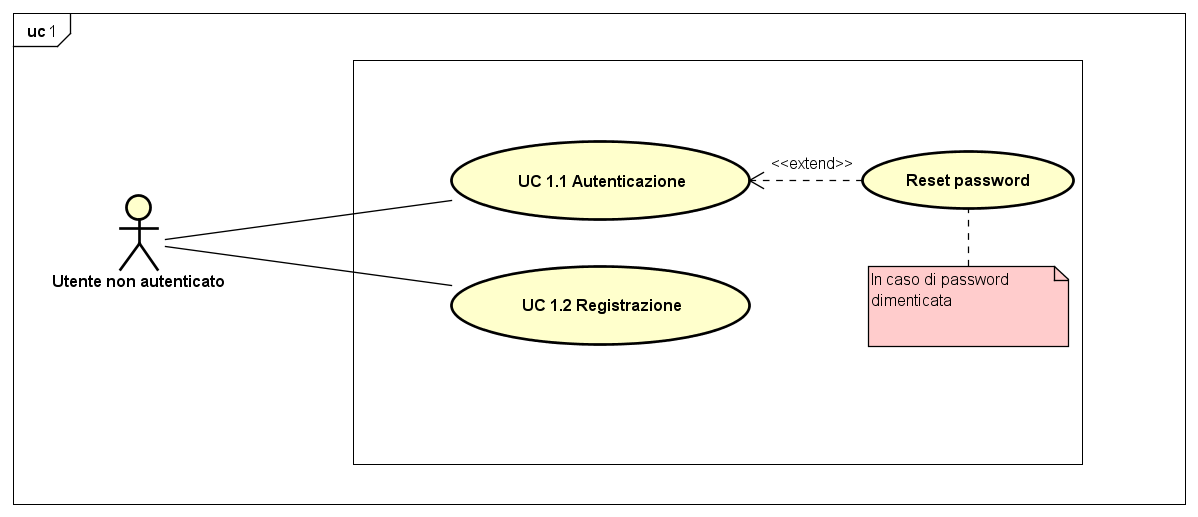
\includegraphics[width=17cm]{img/UC1.png} 
\caption{Panoramica utente non autenticato}\label{fig:1}
\end{figure}


\subsubsection{UC 1.1 - Autenticazione}

\begin{figure}[H]
\centering
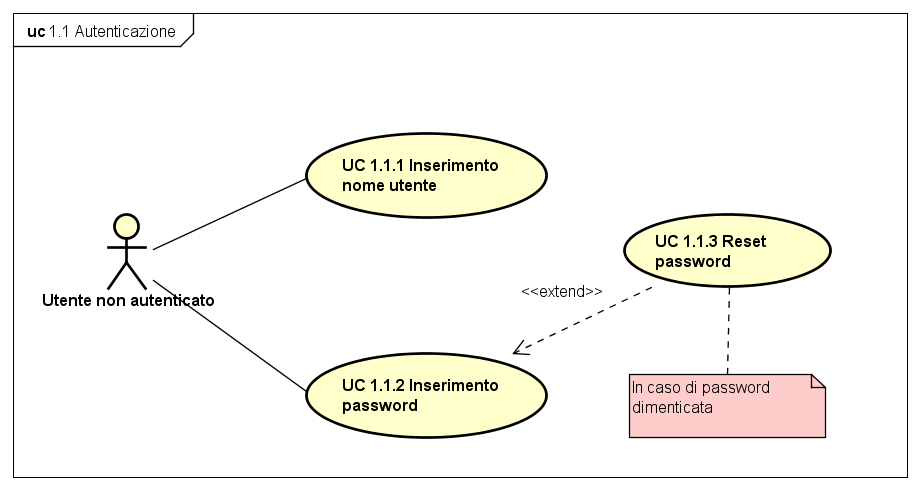
\includegraphics[width=17cm, keepaspectratio]{img/UC11.png} 
\caption{Caso d'uso UC 1.1}
\end{figure}

\begin{itemize}
\item[•]\textbf{Attori}: Utente non autenticato;
\item[•]\textbf{Descrizione}:  l’utente non identificato inserisce email e password e si autentica accedendo alla dashboard;
\item[•]\textbf{Precondizione}: l’utente non è autenticato;
\item[•]\textbf{Postcondizione}: l’utente viene autenticato all’interno del sistema;
\item[•]\textbf{Flusso degli eventi}:
\begin{enumerate}
\item UC 1.1.1 - Inserimento email;
\item UC 1.1.2 - Inserimento password;

\end{enumerate}
\item[•]\textbf{Estensioni}:
\begin{enumerate}
\item UC 1.1.4 - Visualizzazione messaggio credenziali errate.
\end{enumerate}
\end{itemize}

\subsubsection{UC 1.1.1 - Inserimento email}
\begin{itemize}
\item[•]\textbf{Attori}: Utente non autenticato;
\item[•]\textbf{Descrizione}: l’utente inserisce la propria email utilizzata in fase di registrazione;
\item[•]\textbf{Precondizione}: l’utente non è autenticato;
\item[•]\textbf{Postcondizione}: l’utente ha inserito la propria email;
\item[•]\textbf{Flusso degli eventi}: l'utente visualizza il form per l'autenticazione e inserisce l'email utilizzata in fase di registrazione in un apposito campo.

\end{itemize}

\subsubsection{UC 1.1.2 - Inserimento password}
\begin{itemize}
\item[•]\textbf{Attori}: Utente non autenticato;
\item[•]\textbf{Descrizione}: l’utente inserisce una password inserita in fase di registrazione;
\item[•]\textbf{Precondizione}: l'utente non è autenticato;
\item[•]\textbf{Postcondizione}: l'utente ha inserito la password utilizzata in fase di registrazione;
\item[•]\textbf{Flusso degli eventi}: l'utente visualizza il form per l'autenticazione e inserisce la password in apposito campo.
\end{itemize}

\subsubsection{UC 1.1.3 - Visualizzazione messaggio credenziali errate}
\begin{itemize}
\item[•]\textbf{Attori}: Utente non autenticato;
\item[•]\textbf{Descrizione}: l'utente ha avviato il login immettendo delle credenziali errati;
\item[•]\textbf{Precondizione}: l'utente non è autenticato;
\item[•]\textbf{Postcondizione}: l'utente riceve un messaggio d'errore per aver inserito email o password con valori errati;
\item[•]\textbf{Flusso degli eventi}: l'utente visualizza il form per l'autenticazione, inserisce email e password in appositi campi, riscontrando errore sulle credenziali.
\end{itemize}

\subsubsection{UC 1.2 - Registrazione utente}
\begin{figure}[H]
	\centering
	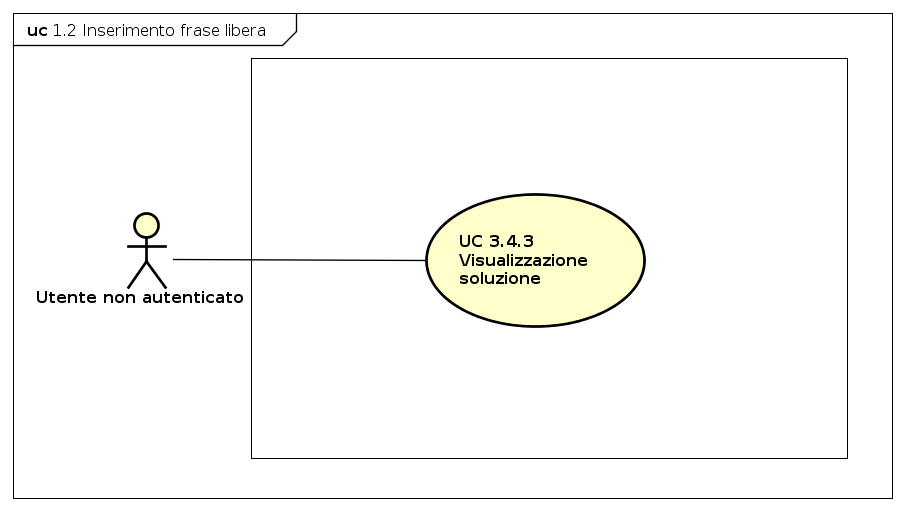
\includegraphics[width=17cm]{img/UC12.png} 
	\caption{Caso d'uso UC 1.2}\label{fig:12}
\end{figure}
\begin{itemize}
	\item[•]\textbf{Attori}: Utente non autenticato;
	\item[•]\textbf{Descrizione}: l'utente non autenticato compila il modulo di registrazione al fine di poter accedere al sistema;
	\item[•]\textbf{Precondizione}: l'utente non è autenticato;
	\item[•]\textbf{Postcondizione}: l'utente si è registrato e può quindi accedere al sistema;
	\item[•]\textbf{Flusso degli eventi}:
	\begin{enumerate}
		\item UC 1.2.1 - Inserimento email;
		\item UC 1.2.2 - Inserimento nome;
		\item UC 1.2.3 - Inserimento cognome;
		\item UC 1.2.4 - Inserimento password;
		\item UC 1.2.5 - Inserimento conferma password;
		\item UC 1.2.6 - Inserimento data di nascita;
		\item UC 1.2.7 - Selezione ruolo.
	\end{enumerate}
	\item[•]\textbf{Estensioni}:
	\begin{enumerate}
		\item UC 1.3 - Visualizzazione messaggio errore dato presente;
		\item UC 1.4 - Visualizzazione messaggio errore password diverse;
		\item UC 1.7 - Interruzione registrazione utente.
	\end{enumerate}
\end{itemize}

\subsubsection{UC 1.2.1 - Inserimento e-mail}
\begin{itemize}
	\item[•]\textbf{Attori}: Utente non autenticato;
	\item[•]\textbf{Descrizione}: l'utente inserisce la sua email durante la registrazione;
	\item[•]\textbf{Precondizione}: l'utente non è autenticato e la email non è definita;
	\item[•]\textbf{Postcondizione}: l'utente ha inserito la propria email;
	\item[•]\textbf{Flusso degli eventi}: l'utente visualizza il form per la registrazione e inserisce la propria e-mail in apposito campo;
	\item[•] \textbf{Estensioni}:
		\begin{enumerate}
		\item UC 1.3 - Visualizzazione messaggio errore dato presente.
	\end{enumerate}
\end{itemize}

\subsubsection{UC 1.2.2 - Inserimento nome}
\begin{itemize}
\item[•]\textbf{Attori}: Utente non autenticato;
\item[•]\textbf{Descrizione}: l'utente inserisce il suo nome durante la registrazione;
\item[•]\textbf{Precondizione}: l'utente non è autenticato e il nome non è definito;
\item[•]\textbf{Postcondizione}: l'utente ha inserito il suo nome;
\item[•]\textbf{Flusso degli eventi}: l'utente visualizza il form per la registrazione e inserisce il suo nome in un apposito campo;
	\item[•]\textbf{Estensioni}:
	\begin{enumerate}
		\item UC 1.7 - Interruzione registrazione utente.
	\end{enumerate}
\end{itemize}

\subsubsection{UC 1.2.3 - Inserimento cognome}
\begin{itemize}
	\item[•]\textbf{Attori}: Utente non autenticato;
	\item[•]\textbf{Descrizione}: l'utente inserisce il suo cognome durante la registrazione;
	\item[•]\textbf{Precondizione}: l'utente non è autenticato e il cognome non è definito;
	\item[•]\textbf{Postcondizione}: l'utente ha inserito il suo cognome;
	\item[•]\textbf{Flusso degli eventi}: l'utente visualizza il form per la registrazione e inserisce il suo cognome in un apposito campo;
	\item[•]\textbf{Estensioni}:
	\begin{enumerate}
		\item UC 1.7 - Interruzione registrazione utente.
	\end{enumerate}
\end{itemize}

\subsubsection{UC 1.2.4 - Inserimento password}
\begin{itemize}
	\item[•]\textbf{Attori}: Utente non autenticato;
	\item[•]\textbf{Descrizione}: l'utente inserisce una password durante procedura di registrazione;
	\item[•]\textbf{Precondizione}: l'utente non è autenticato e la password non è definita;
	\item[•]\textbf{Postcondizione}: l'utente ha inserito una password;
	\item[•]\textbf{Flusso degli eventi}: l'utente visualizza il form per la registrazione e inserisce la propria password in apposito campo;
	\item[•]\textbf{Estensioni}:
	\begin{enumerate}
		\item UC 1.7 - Interruzione registrazione utente.
	\end{enumerate}
\end{itemize}

\subsubsection{UC 1.2.5 - Inserimento conferma password}
\begin{itemize}
	\item[•]\textbf{Attori}: Utente non autenticato;
	\item[•]\textbf{Descrizione}: l'utente inserisce la conferma della password durante la registrazione;
	\item[•]\textbf{Precondizione}: l'utente non è autenticato e la conferma password non è definita;
	\item[•]\textbf{Postcondizione}: l'utente ha inserito la conferma della password;
	\item[•]\textbf{Flusso degli eventi}: l'utente visualizza il form per la registrazione e inserisce, confermando per la seconda volta, la propria password in un apposito campo e conferma la password;
	\item[•] \textbf{Estensioni}:
		\begin{enumerate}
		\item UC 1.4 - Visualizzazione messaggio errore password diverse.
	\end{enumerate}
\end{itemize}

\subsubsection{UC 1.2.6 - Inserimento data di nascita}
\begin{itemize}
	\item[•]\textbf{Attori}: Utente non autenticato;
	\item[•]\textbf{Descrizione}: l'utente inserisce la sua data di nascita durante la registrazione;
	\item[•]\textbf{Precondizione}: l'utente non è autenticato e la data di nascita non è definita;
	\item[•]\textbf{Postcondizione}: l'utente ha inserito la sua data di nascita;
	\item[•]\textbf{Flusso degli eventi}: l'utente visualizza il form per la registrazione e inserisce la data di nascita in un apposito campo;
	\item[•]\textbf{Estensioni}:
	\begin{enumerate}
		\item UC 1.7 - Interruzione registrazione utente.
	\end{enumerate}
\end{itemize}

\subsubsection{UC 1.2.7 - Selezione ruolo}
\begin{itemize}
	\item[•]\textbf{Attori}: Utente non registrato;
	\item[•]\textbf{Descrizione}: l'utente seleziona il ruolo che vorrebbe ricoprire all'interno dell'applicativo;
	\item[•]\textbf{Precondizione}: l'utente non è registrato e il ruolo non è definito;
	\item[•]\textbf{Postcondizione}: l'utente ha inserito il ruolo desiderato;
	\item[•]\textbf{Flusso degli eventi}: l'utente non registrato seleziona la scelta del ruolo tra: allievo, insegnante e sviluppatore;
	\item[•]\textbf{Estensioni}:
	\begin{enumerate}
		\item UC 1.7 - Interruzione registrazione utente;
	\end{enumerate}
	\item[•]\textbf{Generalizzazioni}: 
	\begin{enumerate}
		\item UC 1.2.7.1 - Selezione ruolo insegnante;
		\item UC 1.2.7.2 - Selezione ruolo allievo;
		\item UC 1.2.7.3 - Selezione ruolo sviluppatore.
	\end{enumerate}
\end{itemize}

\subsubsection{UC 1.2.7.1 - Selezione ruolo insegnante}
\begin{itemize}
	\item[•]\textbf{Attori}: Utente non registrato;
	\item[•]\textbf{Descrizione}: l'utente seleziona il ruolo insegnante per registrarsi con tale ruolo all'interno dell'applicativo;
	\item[•]\textbf{Precondizione}: l'utente non è registrato e il ruolo non è selezionato;
	\item[•]\textbf{Postcondizione}: l'utente ha selezionato il ruolo insegnante;
	\item[•]\textbf{Flusso degli eventi}: l'utente non registrato seleziona il ruolo insegnante da un elenco predefinito;
	\item[•]\textbf{Estensioni}:
	\begin{enumerate}
		\item UC 1.7 - Interruzione registrazione utente.
	\end{enumerate}
\end{itemize}
\subsubsection{UC 1.2.7.2 - Selezione ruolo allievo}
\begin{itemize}
	\item[•]\textbf{Attori}: Utente non registrato;
	\item[•]\textbf{Descrizione}: l'utente seleziona il ruolo allievo per registrarsi con tale ruolo all'interno dell'applicativo;
	\item[•]\textbf{Precondizione}: l'utente non è registrato e il ruolo non è selezionato;
	\item[•]\textbf{Postcondizione}: l'utente ha selezionato il ruolo allievo;
	\item[•]\textbf{Flusso degli eventi}: l'utente non registrato seleziona il ruolo allievo da un elenco predefinito;
	\item[•]\textbf{Estensioni}:
	\begin{enumerate}
		\item UC 1.7 - Interruzione registrazione utente.
	\end{enumerate}
\end{itemize}
\subsubsection{UC 1.2.7.3 - Selezione ruolo sviluppatore}
\begin{itemize}
	\item[•]\textbf{Attori}: Utente non registrato;
	\item[•]\textbf{Descrizione}: l'utente seleziona il ruolo sviluppatore per registrarsi con tale ruolo all'interno dell'applicativo;
	\item[•]\textbf{Precondizione}: l'utente non è registrato e il ruolo non è selezionato;
	\item[•]\textbf{Postcondizione}: l'utente ha selezionato il ruolo sviluppatore;
	\item[•]\textbf{Flusso degli eventi}: l'utente non registrato seleziona il ruolo sviluppatore da un elenco predefinito;
	\item[•]\textbf{Estensioni}:
	\begin{enumerate}
		\item UC 1.7 - Interruzione registrazione utente.
	\end{enumerate}
\end{itemize}


\subsubsection{UC 1.3 - Visualizzazione messaggio errore dato presente}
\begin{itemize}
	\item[•]\textbf{Attori}: Utente non registrato;
	\item[•]\textbf{Descrizione}: l'utente non registrato visualizza un messaggio di errore relativo all'inserimento
	di un dato già presente nel sistema;
	\item[•]\textbf{Precondizione}: l'utente non registrato sta completando la procedura di registrazione;
	\item[•]\textbf{Postcondizione}: l'utente visualizza un messaggio di errore relativo all'inserimento di un valore già presente nel sistema;
	\item[•]\textbf{Flusso degli eventi}: l'utente inserisce una email già presente nel sistema, pertanto riceve un messaggio di errore.
\end{itemize}

\subsubsection{UC 1.4 - Visualizzazione messaggio errore password diverse}
\begin{itemize}
	\item[•]\textbf{Attori}: Utente non registrato;
	\item[•]\textbf{Descrizione}: l'utente non registrato visualizza un messaggio che comunica che i valori della password e di conferma password sono tra loro diversi;
	\item[•]\textbf{Precondizione}: l'utente non registrato ha inserito la conferma password con valore differente rispetto alla password precedentemente inserita;
	\item[•]\textbf{Postcondizione}: l'utente visualizza un messaggio di errore relativo all'inserimento di password e conferma password con valori diversi;
	\item[•]\textbf{Flusso degli eventi}: l'utente inserisce conferma password con un valore differente rispetto al campo password, pertanto riceve un messaggio di errore.
\end{itemize}

\subsubsection{UC 1.5 - Recupero credenziali}
\begin{figure}[H]
	\centering
	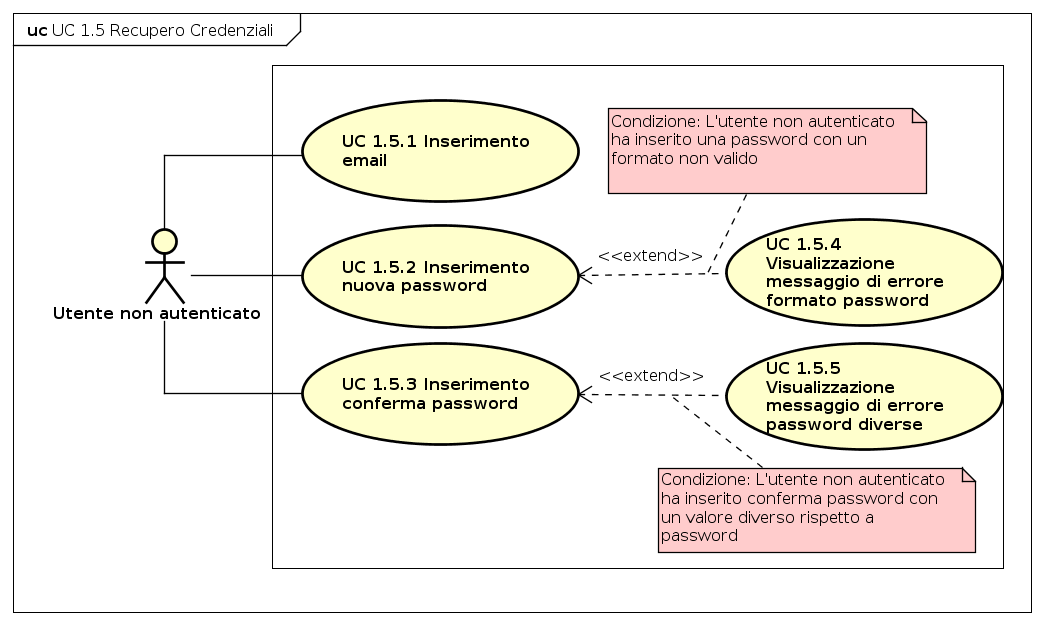
\includegraphics[width=14cm, keepaspectratio]{img/UC15.png} 
	\caption{Caso d'uso UC 1.5}\label{fig:15}
\end{figure}
\begin{itemize}
	\item[•]\textbf{Attori}: Utente non autenticato;
	\item[•]\textbf{Descrizione}: l’utente avvia iter per il recupero delle proprie credenziali smarrite;
	\item[•]\textbf{Precondizione}: l’utente non è autenticato;
	\item[•]\textbf{Postcondizione}: l’utente ha inviato la richiesta di recupero;
	\item[•]\textbf{Flusso degli eventi}:
	\begin{enumerate}
	\item Selezione procedura recupero credenziali;
	\item UC 1.5.1 - Inserimento email;
	\item Conferma smarrimento credenziali;
	\item UC 1.5.2 - Inserimento nuova password;
	\item UC 1.5.3 - Inserimento conferma password;
	\item Conferma modifica password;
	\end{enumerate}
	\item[•]\textbf{Estensioni}:
	\begin{enumerate}
		\item UC 1.5.6 - Interruzione recupero credenziali.
	\end{enumerate}
\end{itemize}

%\subsubsection{UC 1.5.1 - Selezione procedura recupero credenziali}
%\begin{itemize}
%	\item[•]\textbf{Attori}: Utente non autenticato;
%	\item[•]\textbf{Descrizione}: l’utente seleziona il collegamento che conduce alla pagina di recupero delle credenziali;
%	\item[•]\textbf{Precondizione}: l’utente non è autenticato;
%	\item[•]\textbf{Postcondizione}: l’utente visualizza la pagina di recupero delle credenziali;
%	\item[•]\textbf{Flusso degli eventi}: l'utente non autenticato seleziona l'opzione per il recupero delle credenziali e viene automaticamente reindirizzato alla pagina di recupero. 
%\end{itemize}

\subsubsection{UC 1.5.1 - Inserimento email}
\begin{itemize}
	\item[•]\textbf{Attori}: Utente non autenticato;
	\item[•]\textbf{Descrizione}: l’utente non autenticato inserisce l'email utilizzata in fase di registrazione;
	\item[•]\textbf{Precondizione}: l’utente non è autenticato;
	\item[•]\textbf{Postcondizione}: l’utente ha inserito la email utilizzata in fase di registrazione;
	\item[•]\textbf{Flusso degli eventi}: l'utente non autenticato inserisce una stringa che rappresenta la email utilizzata in fase di registrazione. 
\end{itemize}

%\subsubsection{UC 1.5.3 - Conferma smarrimento credenziali}
%\begin{itemize}
%	\item[•]\textbf{Attori}: Utente non autenticato;
%	\item[•]\textbf{Descrizione}: l’utente non autenticato conferma lo smarrimento delle credenziali;
%	\item[•]\textbf{Precondizione}: l’utente non è autenticato;
%	\item[•]\textbf{Postcondizione}: l’utente ha confermato lo smarrimento delle credenziali. Il sistema provvede a inviare una mail con il collegamento per il recupero password;
%	\item[•]\textbf{Flusso degli eventi}: l'utente non autenticato conferma lo smarrimento delle credenziali. 
%\end{itemize}

\subsubsection{UC 1.5.2 - Inserimento nuova password}
\begin{itemize}
	\item[•]\textbf{Attori}: Utente non autenticato;
	\item[•]\textbf{Descrizione}: l’utente non autenticato inserisce la nuova password;
	\item[•]\textbf{Precondizione}: l’utente non autenticato visualizza il contenuto del collegamento ricevuto tramite email;
	\item[•]\textbf{Postcondizione}: l'utente ha inserito la nuova password;
	\item[•]\textbf{Flusso degli eventi}: l'utente non autenticato seleziona il campo di input relativo all'inserimento della nuova password e inserisce una stringa che rappresenta la nuova password;
	\item[•]\textbf{Estensioni}:
	\begin{enumerate}
		\item UC 1.5.4 - Visualizzazione messaggio di errore formato password.
	\end{enumerate}
\end{itemize}

\subsubsection{UC 1.5.3 - Inserimento conferma password}
\begin{itemize}
	\item[•]\textbf{Attori}: Utente non autenticato;
	\item[•]\textbf{Descrizione}: l’utente non autenticato re-inserisce la nuova password;
	\item[•]\textbf{Precondizione}: l’utente non autenticato ha inserito la nuova password;
	\item[•]\textbf{Postcondizione}: l'utente ha re-inserito la nuova password;
	\item[•]\textbf{Flusso degli eventi}: l'utente non autenticato seleziona il campo di input relativo all'inserimento della conferma password e re-inserisce la nuova password;
	\item[•]\textbf{Estensioni}:
	\begin{enumerate}
		\item UC 1.5.5 - Visualizzazione messaggio di errore password diverse.
	\end{enumerate}
\end{itemize}

\subsubsection{UC 1.5.4 - Visualizzazione messaggio di errore formato password}
\begin{itemize}
	\item[•]\textbf{Attori}: Utente non autenticato;
	\item[•]\textbf{Descrizione}: l’utente non autenticato visualizza un messaggio di errore in quanto la password inserita non soddisfa i requisiti richiesti;
	\item[•]\textbf{Precondizione}: l’utente non autenticato ha inserito la nuova password;
	\item[•]\textbf{Postcondizione}: l'utente non autenticato visualizza un messaggio di errore relativo all'inserimento di una password che non soddisfa i requisiti richiesti;
	\item[•]\textbf{Flusso degli eventi}: l'utente non autenticato ha inserito una password con un formato non idoneo, pertanto visualizza un messaggio di errore.
\end{itemize}

\subsubsection{UC 1.5.5 - Visualizzazione messaggio di errore password diverse}
\begin{itemize}
	\item[•]\textbf{Attori}: Utente non autenticato;
	\item[•]\textbf{Descrizione}: l’utente non autenticato visualizza un messaggio di errore in quanto la conferma password inserita non ha lo stesso valore della password precedente;
	\item[•]\textbf{Precondizione}: l’utente non autenticato ha inserito la conferma della nuova password;
	\item[•]\textbf{Postcondizione}: l'utente non autenticato visualizza un messaggio di errore relativo all'inserimento della conferma password con un valore diverso dalla password precendentemente inserita;
	\item[•]\textbf{Flusso degli eventi}: l'utente non autenticato ha inserito la conferma password con un valore diverso rispetto alla password precendentemente inserita, pertanto visualizza un messaggio di errore.
\end{itemize}

\subsubsection{UC 1.5.6 - Interruzione recupero credenziali}
\begin{itemize}
	\item[•]\textbf{Attori}: Utente non autenticat;
	\item[•]\textbf{Descrizione}: l'utente non autenticato interrompe il recupero delle credenziali smarrite;
	\item[•]\textbf{Precondizione}: l'utente non autenticato sta recuperando le credenziali;
	\item[•]\textbf{Postcondizione}: l'utente non autenticato interrompe il recupero delle credenziali e torna alla pagina di autenticazione;
	\item[•]\textbf{Flusso degli eventi}: durante il recupero delle credenziali, l'utente generico interrompe la procedura e ritorna nella pagina di autenticazione.
\end{itemize}

%\subsubsection{UC 1.5.6 - Conferma modifica password}
%\begin{itemize}
%	\item[•]\textbf{Attori}: Utente non autenticato;
%	\item[•]\textbf{Descrizione}: l’utente non autenticato conferma la modifica delle password;
%	\item[•]\textbf{Precondizione}: l’utente non autenticato ha inserito la conferma della nuova password (UC 1.5.5);
%	\item[•]\textbf{Postcondizione}: l'utente viene reindirizzato alla pagina di autenticazione;
%	\item[•]\textbf{Flusso degli eventi}: l'utente non autenticato conferma la modifica della password e viene reindirizzato alla pagina di autenticazione.
%\end{itemize}

\subsubsection{UC 1.6 - Selezione lingua interfaccia applicativo}
\begin{itemize}
\item[•]\textbf{Attori}: Utente non autenticato;
\item[•]\textbf{Descrizione}: l’utente seleziona la lingua desiderata per l'interfaccia dell'applicativo;
\item[•]\textbf{Precondizione}: l’utente non è autenticato e il valore della lingua dell'applicativo è basato sulla geo-localizzazione dell'utente o sull'ultima scelta effettuata;
\item[•]\textbf{Postcondizione}: l’utente ha selezionato la lingua desiderata e il sistema mostra l'interfaccia di autenticazione nella lingua scelta;
\item[•]\textbf{Flusso degli eventi}: l'utente visualizza il form per l'autenticazione e seleziona da un elenco predefinito la lingua da utilizzare all'interno del sistema.
\end{itemize}

\subsubsection{UC 1.7 - Interruzione registrazione utente}
\begin{itemize}
	\item[•] \textbf{Attori}: Utente non autenticato;
	\item[•] \textbf{Descrizione}: l’utente non autenticato interrompe la procedura di registrazione;
	\item[•] \textbf{Precondizione}: l'utente non autenticato sta effettuando la procedura di registrazione;
	\item[•] \textbf{Postcondizione}: l'utente non autenticato non si è registrato nell'applicativo;
	\item[•] \textbf{Flusso degli eventi}: l'utente non autenticato durante la procedura di registrazione decide di annullarla, pertanto la procedura termina e l'utente non viene registrato.
\end{itemize}


\newpage

\subsection{Insegnante}

\subsubsection{Panoramica Insegnante}

\begin{figure}[H]
\centering
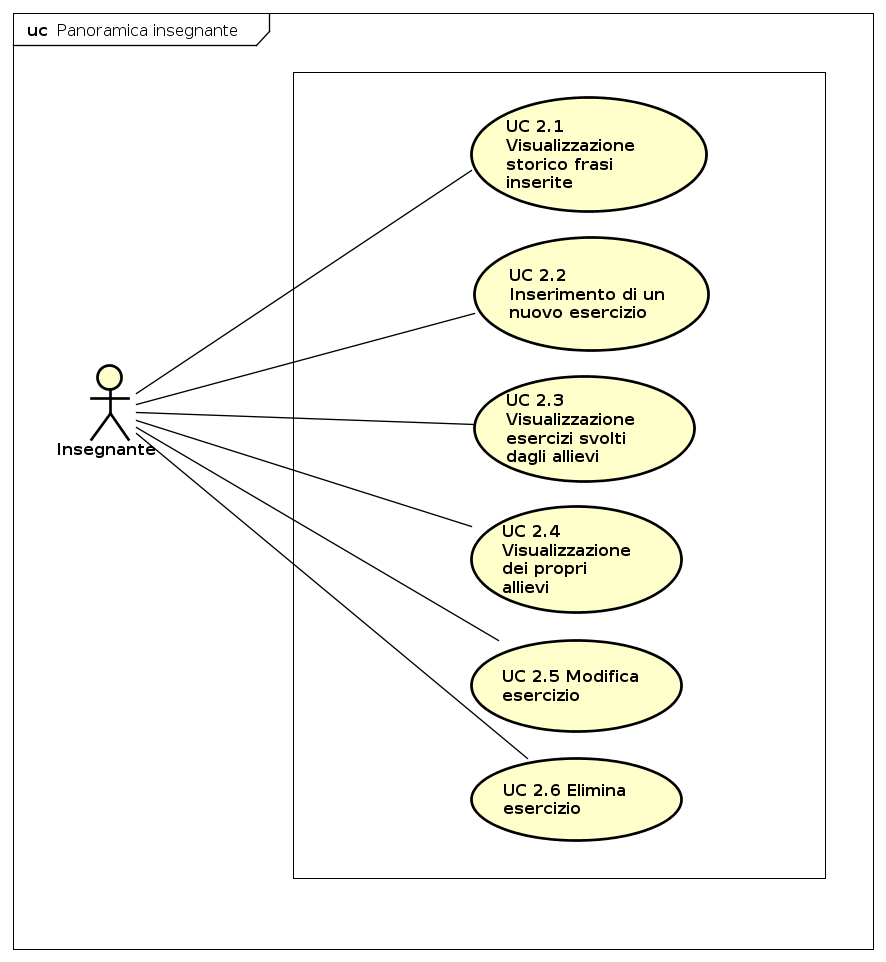
\includegraphics[width=14cm]{img/PanoramicaInsegnanti.png} 
\caption{Panoramica insegnante}
\end{figure}

%MODIFICATO da cambiare uml 
\subsubsection{UC 2.1 Visualizzazione profilo personale}

%\begin{figure}[H]
%\centering
%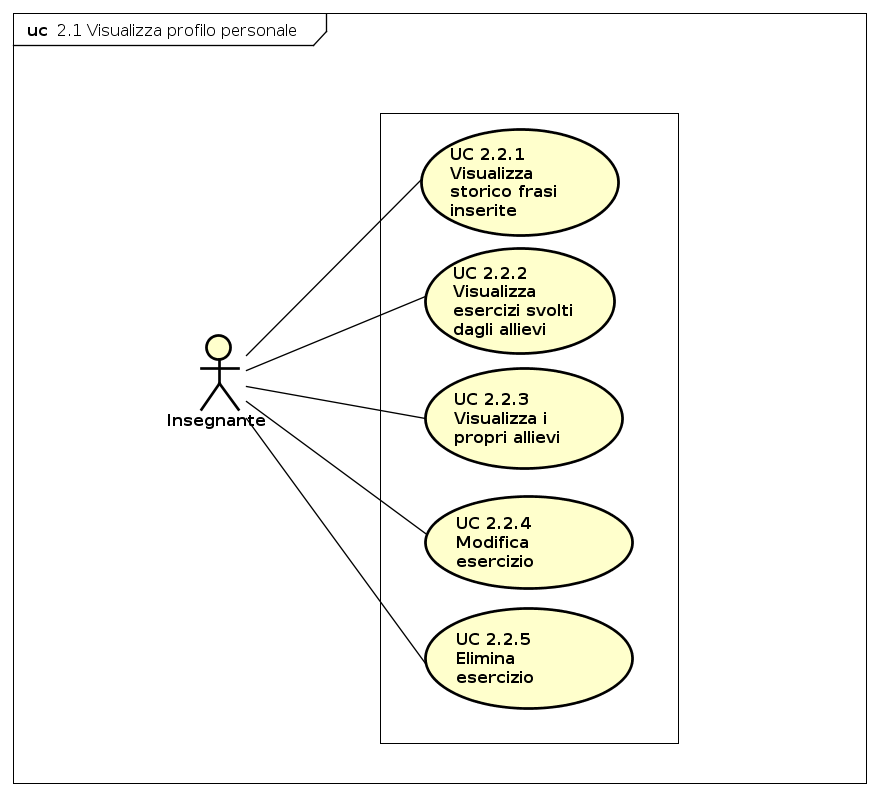
\includegraphics[width=14cm]{img/UC21.png} 
%\caption{Caso d'uso UC 2.1}
%\end{figure}

\begin{itemize}
	\item[•] \textbf{Attori}: Insegnante;
	\item[•] \textbf{Descrizione}: L’insegnante ha accesso al suo profilo personale dove può vedere i suoi dati ed effettuare modifiche agli esercizi;

	\item[•] \textbf{Precondizione}: L'insegnante si è autenticato;

	\item[•] \textbf{Postcondizione}: L'insegnante visualizza il profilo personale.

\end{itemize}


\subsubsection{UC 2.2 Inserimento di un nuovo esercizio}

\begin{figure}[H]
	\centering
	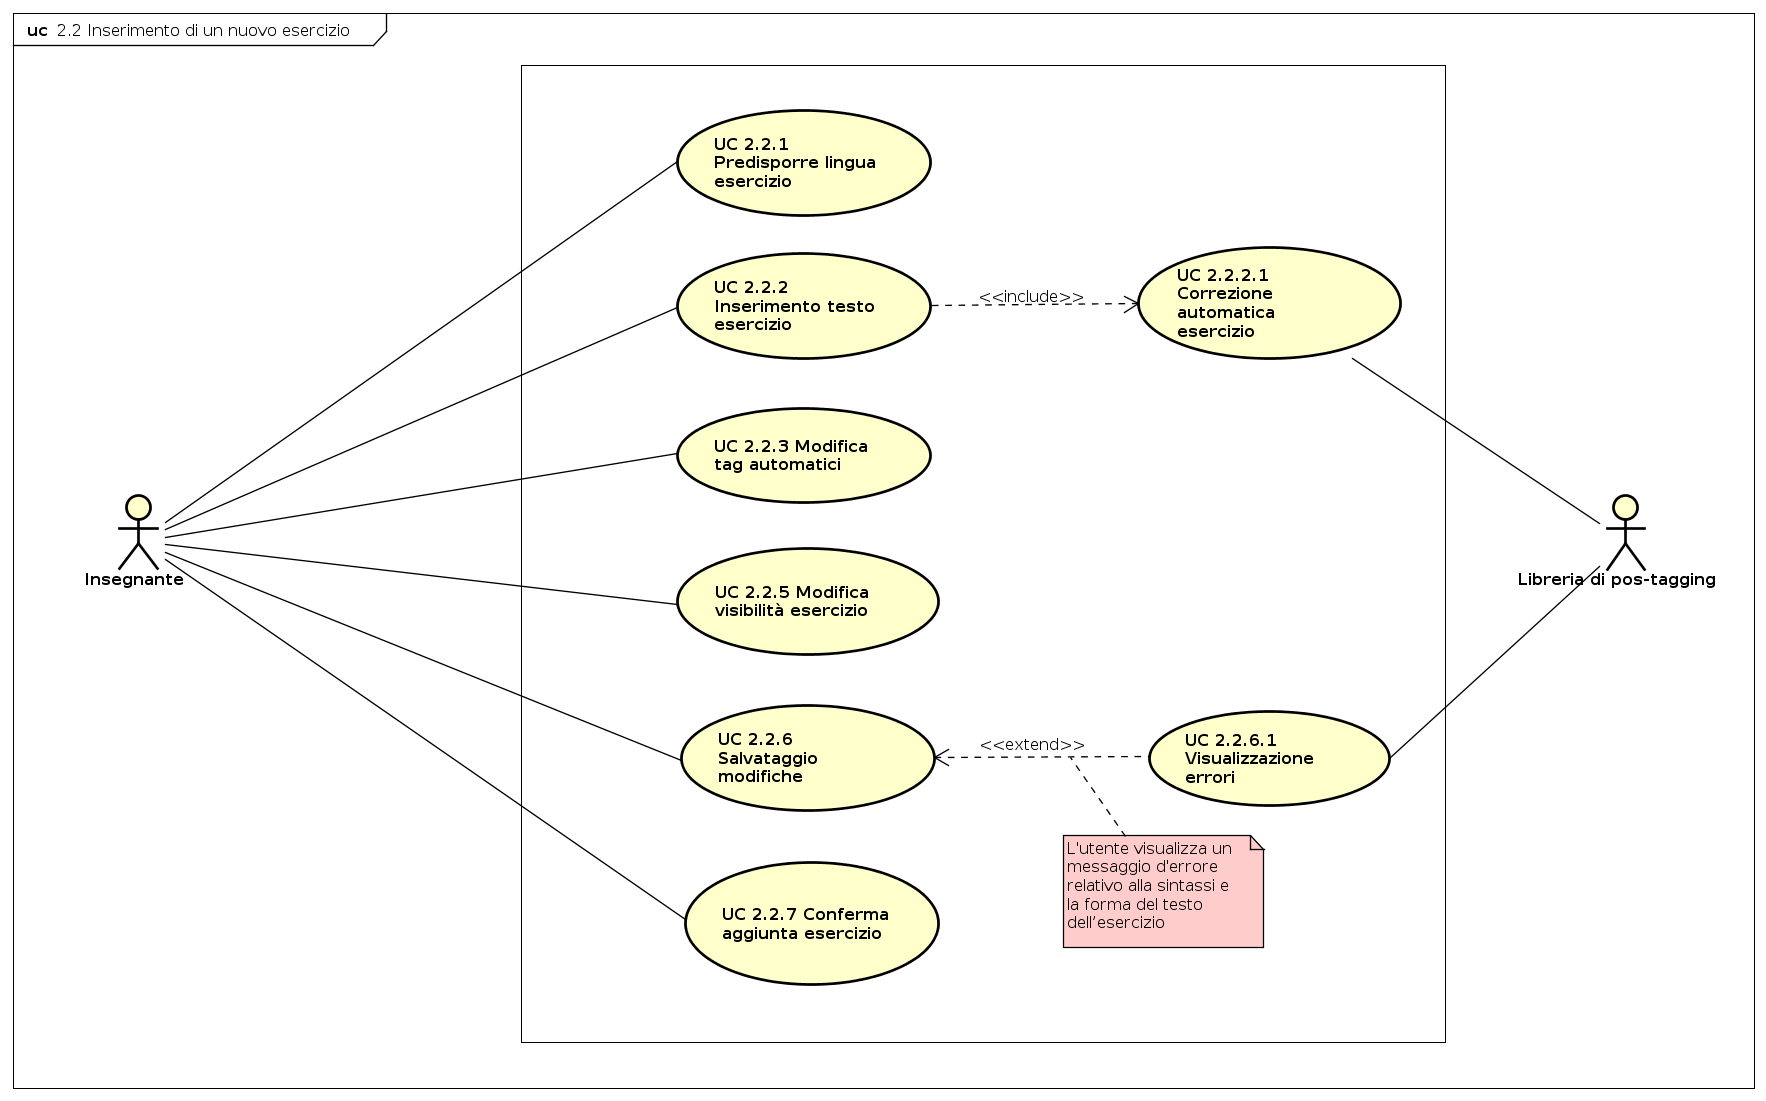
\includegraphics[width=18cm]{img/UC22LIBRERIA.png} 
	\caption{Caso d'uso UC 2.2 interazione con la libreria;}
\end{figure}


\begin{figure}[H]
	\centering
	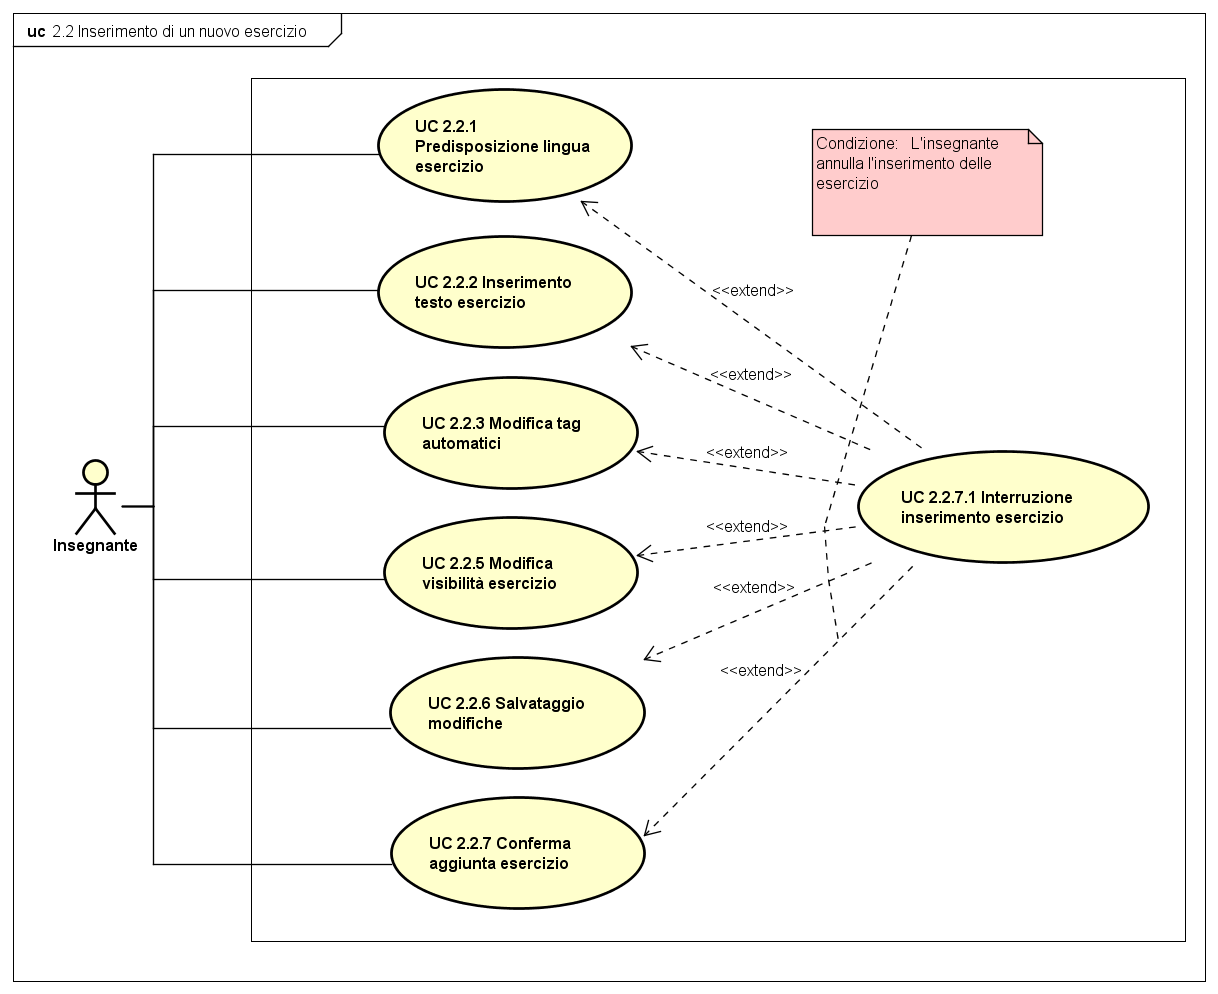
\includegraphics[width=18cm]{img/UC22SISTEMA.png} 
	\caption{Caso d'uso UC 2.2 interazione con il sistema;}
\end{figure}

\begin{itemize}
	\item[•] \textbf{Attori}: Insegnante;
	\item[•] \textbf{Descrizione}: L'insegnante aggiunge un nuovo esercizio;
	\item[•] \textbf{Precondizione}: L'insegnante si è autenticato;
	\item[•] \textbf{Postcondizione}: L'insegnante ha inserito un esercizio;
	\item[•] \textbf{Flusso degli eventi}:
	\begin{enumerate}
		\item UC 2.2.1 Predisporre lingua esercizio;
		\item UC 2.2.2 Inserimento testo esercizio;
		\item UC 2.2.3 Modifica tag automatici;

		\item UC 2.2.5 Modifica visibilità esercizio;
		\item UC 2.2.6 Salvataggio modifiche;
		\item UC 2.2.7 Conferma aggiunta esercizio;
	\end{enumerate}
	\item[•] \textbf{Estensioni}:	
	\begin{enumerate}
		\item UC 2.2.6.1 Visualizzazione errori sintassi testo.
		\item UC 2.2.2.1 Correzione automatica esercizio;
		\item UC 2.2.7.1 Interruzione inserimento esercizio.
	\end{enumerate}
	\item[•] \textbf{Flusso degli eventi alternativo}:
	\begin{enumerate}
		\item UC 2.2.4 Inserimento soluzione alternativa.
	\end{enumerate}
\end{itemize}
%mettere altro sub 
\subsubsection{UC 2.2.1 Predisporre lingua esercizio}
\begin{itemize}
	\item[•] \textbf{Attori}: Insegnante;
	\item[•] \textbf{Descrizione}: L'insegnante sceglie la lingua dell’esercizio che vuole scrivere;
	\item[•] \textbf{Precondizione}: L'insegnante sta inserendo un esercizio;
	\item[•] \textbf{Postcondizione}: L'insegnante ha scelto la lingua dell'esercizio.
\end{itemize}
%mettere altro sub 
\subsubsection{UC 2.2.2 Inserimento testo esercizio}

\begin{itemize}
	\item[•] \textbf{Attori}: Insegnante;
	\item[•] \textbf{Descrizione}: L'insegnante scrive il testo dell’esercizio;
	\item[•] \textbf{Precondizione}: L'insegnante sta inserendo un esercizio;
	\item[•] \textbf{Postcondizione}: L'insegnante ha inserito il testo dell'esercizio.
\end{itemize}

%mettere altro sub 
\subsubsection{UC 2.2.2.1 Correzione automatica esercizio}
\begin{itemize}
	\item[•] \textbf{Attori}: Insegnante, libreria di PoS-tagging;
	\item[•] \textbf{Descrizione}: L’insegnante ottiene automaticamente i tag dal testo dell’esercizio attraverso la libreria di PoS-tagging;
	\item[•] \textbf{Precondizione}: L'insegnante ha inserito il testo dell'esercizio;
	\item[•] \textbf{Postcondizione}: L'insegnante visualizza la soluzione dell'esercizio.
\end{itemize}

%mettere altro sub 
\subsubsection{UC 2.2.3 Modifica tag automatici}
\begin{itemize}
	\item[•] \textbf{Attori}: Insegnante, libreria di PoS-tagging;
	\item[•] \textbf{Descrizione}: L’insegnante modifica i tag generati automaticamente;
	\item[•] \textbf{Precondizione}: L'insegnante visualizza la soluzione dell'esercizio;
	\item[•] \textbf{Postcondizione}: L'insegnante ha modificato i tag generati automaticamente.
\end{itemize}
%mettere altro sub 


\subsubsection{UC 2.2.4 Inserimento soluzione alternativa}
\begin{itemize}
	\item[•] \textbf{Attori}: Insegnante;
	\item[•] \textbf{Descrizione}: L'insegnante, in caso di esercizi con più soluzioni, inserisce tag alternativi all’esercizio;
	\item[•] \textbf{Precondizione}: L'insegnante visualizza la soluzione dell'esercizio;
	\item[•] \textbf{Postcondizione}: L'insegnante aggiunge una soluzione alternativa.
\end{itemize}

%mettere altro sub 
\subsubsection{UC 2.2.5 Modifica visibilità esercizio}
\begin{itemize}
	\item[•] \textbf{Attori}: Insegnante;
	\item[•] \textbf{Descrizione}: L'insegnante imposta la visibilità dell'esercizio, ovvero quali allievi possono visualizzarlo e sceglierlo;
	\item[•] \textbf{Precondizione}: L'insegnante sta inserendo un esercizio;
	\item[•] \textbf{Postcondizione}: L'insegnante ha modificato la visibilità dell'esercizio.
\end{itemize}
%mettere altro sub 
\subsubsection{UC 2.2.6 Salvataggio modifiche}
\begin{itemize}
	\item[•] \textbf{Attori}: Insegnante;
	\item[•] \textbf{Descrizione}: L'insegnante salva l'esercizio e le possibili modifiche;
	\item[•] \textbf{Precondizione}: L'insegnante sta inserendo un esercizio;
	\item[•] \textbf{Postcondizione}: L'insegnante ha salvato l'esercizio.
\end{itemize}
%mettere altro sub 
\subsubsection{UC 2.2.6.1 Visualizzazione errori sintassi testo}
\begin{itemize}
	\item[•] \textbf{Attori}: Insegnante;
	\item[•] \textbf{Descrizione}: L'insegnante visualizza gli errori relativi alla sintassi e la forma del testo che ha inserito;
	\item[•] \textbf{Precondizione}: L'insegnante sta inserendo un esercizio;
	\item[•] \textbf{Postcondizione}: L’insegnante visualizza gli errori relativi al testo inserito.
\end{itemize}
%mettere altro sub 

\subsubsection{UC 2.2.7 Conferma aggiunta esercizio}
\begin{itemize}
	\item[•] \textbf{Attori}: Insegnante;
	\item[•] \textbf{Descrizione}: L'insegnante aggiunge un esercizio al sistema;
	\item[•] \textbf{Precondizione}: L’insegnante sta inserendo un esercizio;
	\item[•] \textbf{Postcondizione}: L'insegnante conferma l'inserimento dell'esercizio.
\end{itemize}





%%%%%%%%%%%%%%%%%%%%
%%%%%% CODICE DA CAMBIARE TUTTI , SI PARTE DA QUI CON UC 2.3 %%%%%%%%%%
%%%%%%%%%%%%%%%%%%%%

\subsubsection{UC 2.3 Visualizzazione storico frasi inserite}

%\begin{figure}[H]
%\centering
%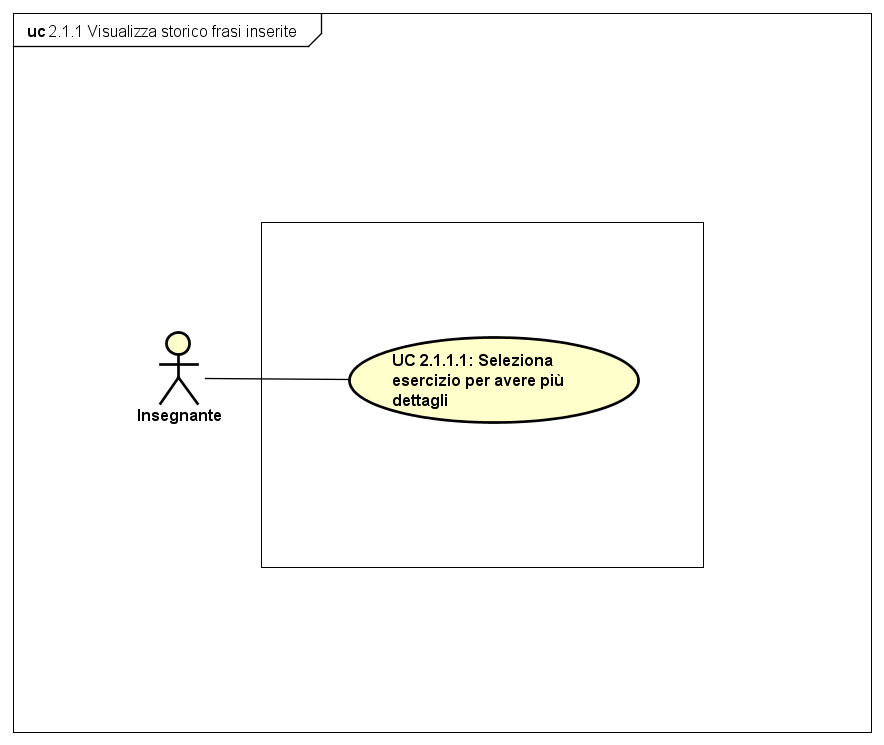
\includegraphics[width=10cm]{img/UC211.png} 
%\caption{Caso d'uso UC 2.1.1}
%\end{figure}

\begin{itemize}
	\item[•] \textbf{Attori}: Insegnante	   
	\item[•] \textbf{Descrizione}: L’insegnante visualizza nel suo profilo personale lo storico delle frasi inserite; 
	\item[•] \textbf{Precondizione}: L'insegnante sta visualizzando il proprio profilo personale;
	\item[•] \textbf{Postcondizione}: L’insegnante può navigare all’interno della lista di frasi che ha inserito.
\end{itemize}

%mettere altro sub 
\subsubsection{UC 2.3.1 Seleziona esercizio per avere più dettagli}
\begin{itemize}
	\item[•] \textbf{Attori}: Insegnante;
	\item[•] \textbf{Descrizione}: L’insegnante seleziona dalla lista degli esercizi assegnati un esercizio e ne visualizza i dettagli;
	\item[•] \textbf{Precondizione}: Linsegnante visualizza la lista di frasi che ha inserito;
	\item[•] \textbf{Postcondizione}: L’insegnante visualizza i dettagli di un esercizio inserito.
\end{itemize}



%DEVE diventare UC 2.4 DA CAMBIARE TUTTO QUANTO 
\subsubsection{UC 2.4 Visualizzazione esercizi svolti dagli allievi}
%\begin{figure}[H]
%\centering
%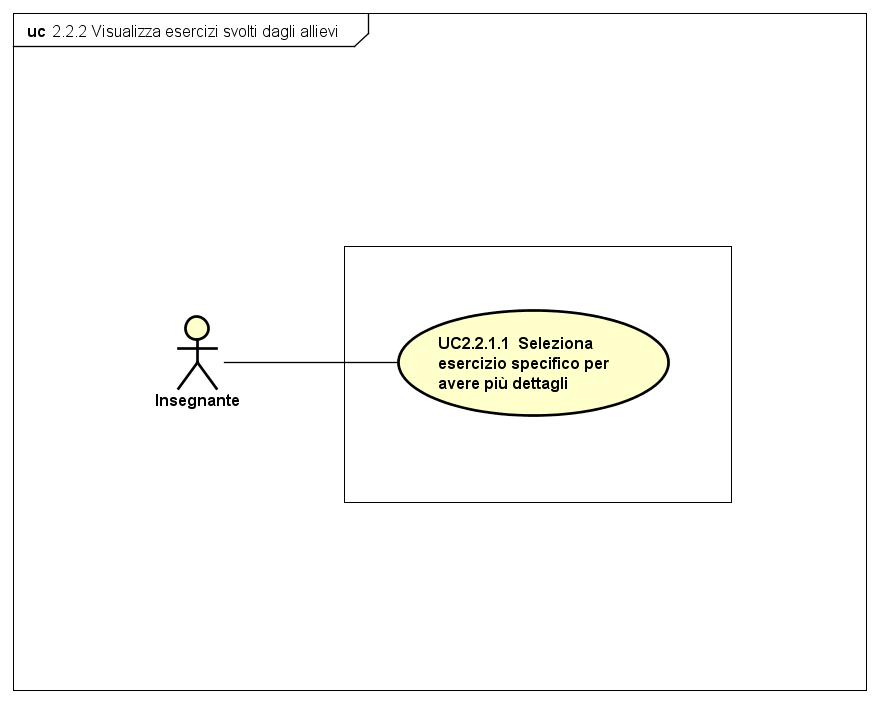
\includegraphics[width=10cm]{img/UC212.png} 
%\caption{Caso d'uso UC 2.1.2}
%\end{figure}
\begin{itemize}
	\item[•] \textbf{Attori}: Insegnante;
	\item[•] \textbf{Descrizione}:  L’insegnante è nella sezione profilo personale e visualizza l’elenco degli esercizi svolti dagli allievi;
	\item[•] \textbf{Precondizione}:  L’insegnante ha assegnato degli esercizi agli allievi che sono stati svolti;

	\item[•] \textbf{Postcondizione}: L’insegnante visualizza l'elenco degli esercizi svolti svolti dagli allievi; 	
\end{itemize}

\subsubsection{UC 2.5 Visualizzazione dei propri allievi}

%\begin{figure}[H]
%\centering
%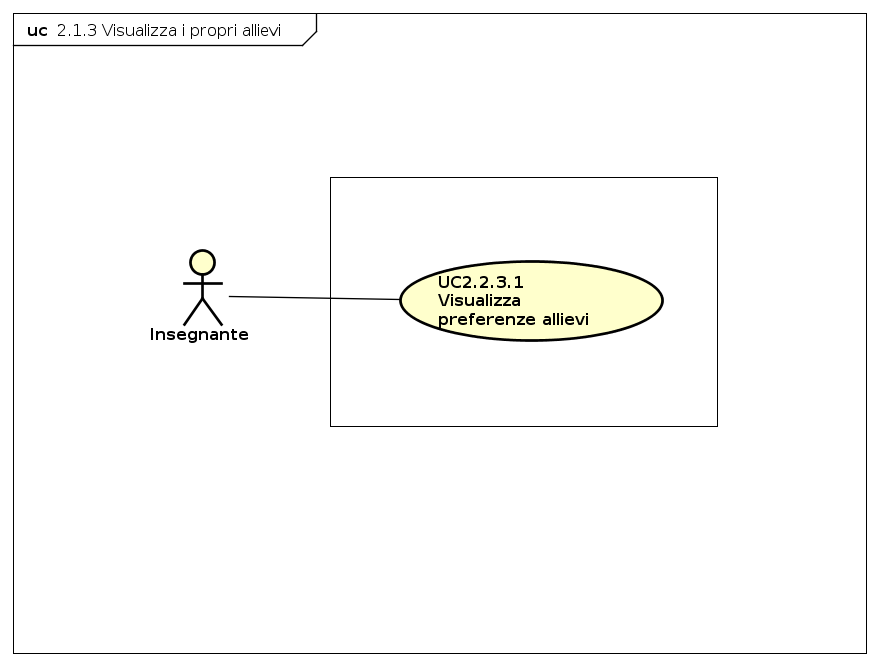
\includegraphics[width=10cm]{img/UC213.png} 
%\caption{Caso d'uso UC 2.1.3}
%\end{figure}

\begin{itemize}
	\item[•] \textbf{Attori}: Insegnante;
	\item[•] \textbf{Descrizione}: L’insegnante visualizza la lista dei suoi allievi;
	\item[•] \textbf{Precondizione}: L'insegnante sta visualizzando il proprio profilo personale;
	\item[•] \textbf{Postcondizione}: L’insegnante visualizza la lista dei propri allievi;
\end{itemize}

%%% da cambiare NUMERO UC va in MODIFICA ESERCIZIO %%%%%%%%%%%%%%


\subsubsection{UC 2.6 Modifica esercizio}
\begin{figure}[H]
\centering
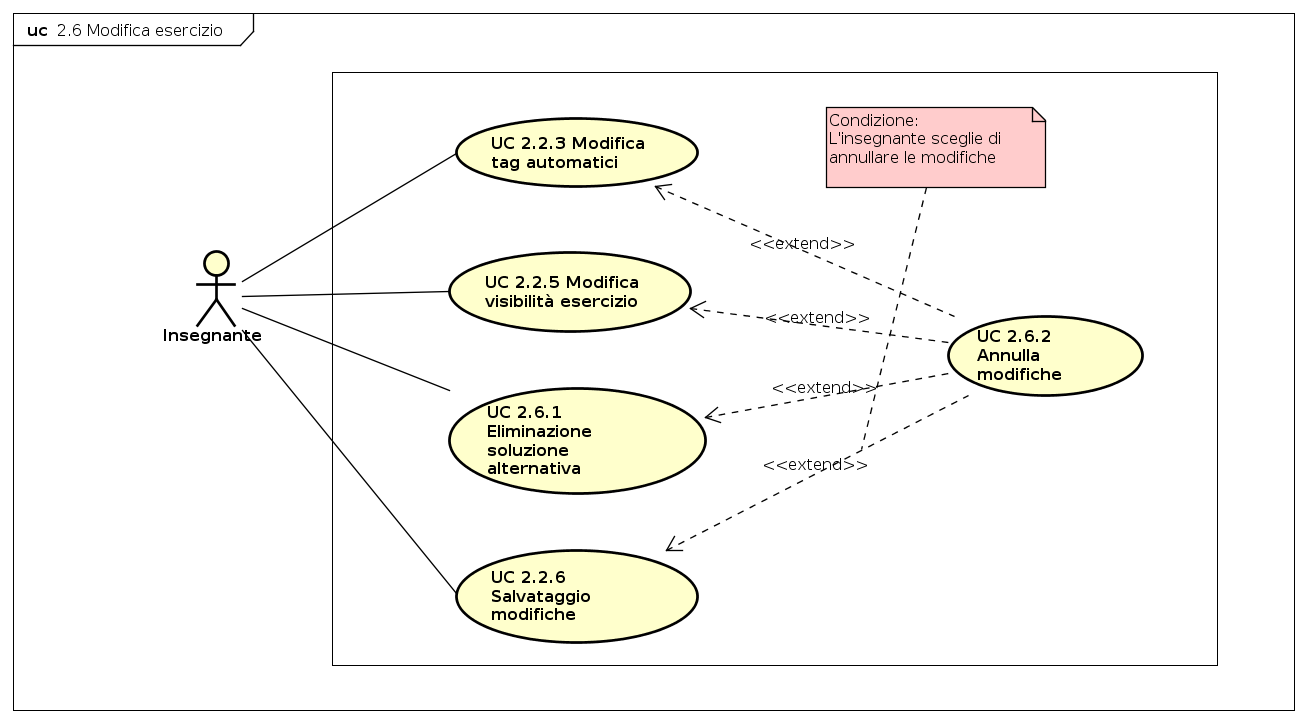
\includegraphics[width=14cm]{img/UC26.png} 
\caption{Caso d'uso UC 2.6}
\end{figure}

\begin{itemize}
	\item[•] \textbf{Attori}: Insegnante;
	\item[•] \textbf{Descrizione}: L’insegnante può modificare il testo, la lingua, la visibilità, i tag e le soluzioni alternative di un esercizio precedentemente inserito;
	\item[•] \textbf{Precondizione}: L'insegnante visualizza i dettagli di un esercizio inserito;
	\item[•] \textbf{Postcondizione}: L’insegnante ha modificato l'esercizio;
	\item[•] \textbf{Flusso degli eventi}:
		\begin{enumerate}
			\item UC 2.2.3 Modifica tag automatici;
			\item UC 2.2.5 Modifica visibilità esercizio;
			\item UC 2.6.1 Elimina soluzione alternativa;
			\item UC 2.2.6 Salvataggio modifiche.
		\end{enumerate}
	\item[•] \textbf{Estensioni}
	\begin{enumerate}
		\item UC 2.6.2 Annulla modifiche.
	\end{enumerate}
\end{itemize}   

\subsubsection{UC 2.6.1 Eliminazione soluzione alternativa}
\begin{itemize}
	\item[•] \textbf{Attori}: Insegnante;
	\item[•] \textbf{Descrizione}: L'insegnante elimina una delle soluzioni alternative inserite in precedenza;
	\item[•] \textbf{Precondizione}: L'insegnante sta modificando un esercizio;
	\item[•] \textbf{Postcondizione}: L'Insegnante ha eliminato una soluzione alternativa di un esercizio.
\end{itemize}

\subsubsection{UC 2.6.2 Annulla modifiche}
\begin{itemize}
	\item[•] \textbf{Attori}: Insegnante;
	\item[•] \textbf{Descrizione}: L'insegnante annulla le modifiche inserite all'interno di un esercizio; 
	\item[•] \textbf{Precondizione}: L'insegnante sta modificando un esercizio;
	\item[•] \textbf{Postcondizione}: L'esercizio non è modificato.
\end{itemize}


 
\subsubsection{UC 2.7 Eliminazione esercizio}
\begin{itemize}
	\item[•] \textbf{Attori}: Insegnante;
	\item[•] \textbf{Descrizione}: L'insegnante ha la possibilità di eliminare un esercizio da lei precedentemente inserito;
	\item[•] \textbf{Precondizione}: L'insegnante visualizza nel suo profilo personale lo storico delle frasi inserite;
	\item[•] \textbf{Postcondizione}: L'insegnante ha eliminato l'esercizio precedentemente inserito.
\end{itemize}
\newpage
\subsection{Allievi}
\subsubsection{Panoramica allievo}

\begin{figure}[H]
\centering
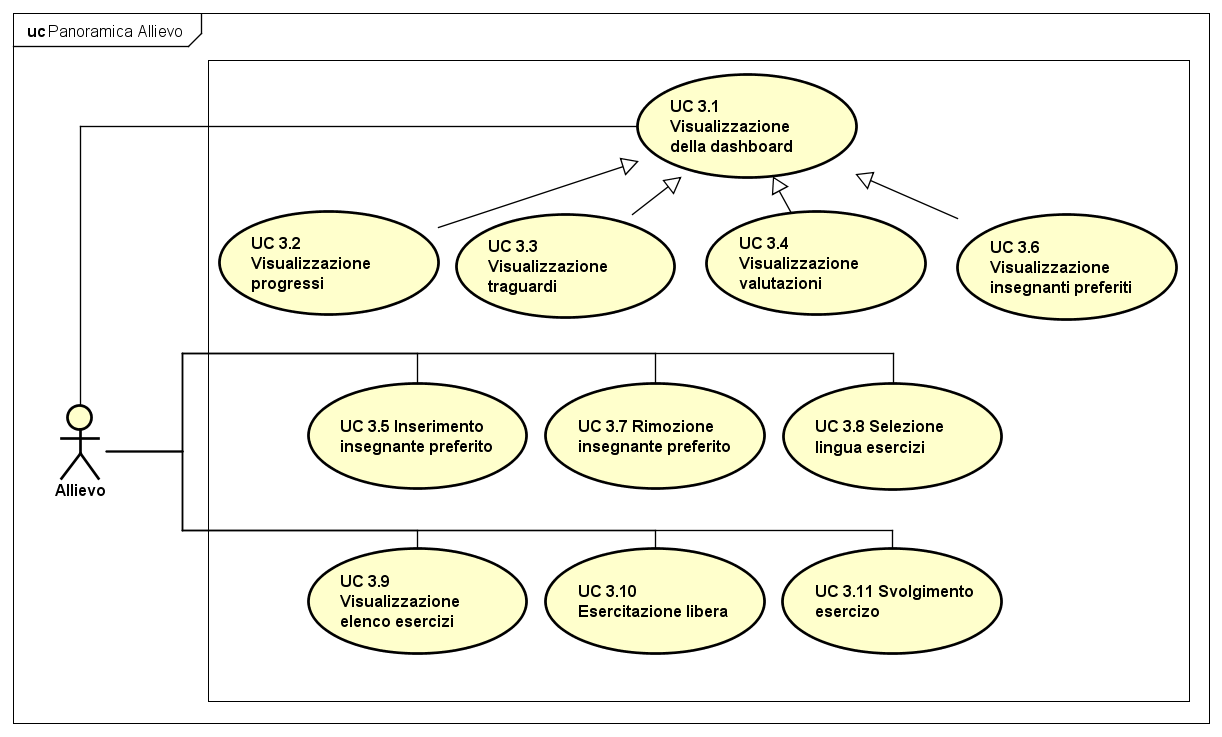
\includegraphics[width=17cm]{img/PanoramicaAllievi.png} 
\caption{Panoramica allievo}\label{fig:31}
\end{figure}


\subsubsection{UC 3.1 - Visualizzazione della dashboard}
\begin{itemize}
\item[•]\textbf{Attori}: Allievo;
\item[•]\textbf{Descrizione}: l'allievo accede alla propria dashboard visualizzando i seguenti contenuti: progressi, traguardi, valutazione esercizi, insegnanti preferiti, elenco esercizi svolti, svolgi esercizio;
\item[•]\textbf{Precondizione}: l'allievo si è autenticato;
\item[•]\textbf{Postcondizione}: l'allievo visualizza la dashboard;
\item[•]\textbf{Flusso degli eventi}: l'allievo ha effettuato il login e viene reinderizzato alla propria dashboard.
\end{itemize}

\subsubsection{UC 3.2 - Visualizzazione progressi}
\begin{itemize}
\item[•]\textbf{Attori}: Allievo;
\item[•]\textbf{Descrizione}: l'allievo visualizza i suoi progressi;
\item[•]\textbf{Precondizione}: l'allievo visualizza la propria dashboard;
\item[•]\textbf{Postcondizione}: l'allievo visualizza i propri progressi;
\item[•]\textbf{Flusso degli eventi}:
\begin{enumerate}
	\item Visualizzazione numero esercizi corretti;
	\item Visualizzazione punteggio medio.
\end{enumerate}
\end{itemize}

\subsubsection{UC 3.3 - Visualizzazione traguardi}

\begin{figure}[H]
\centering
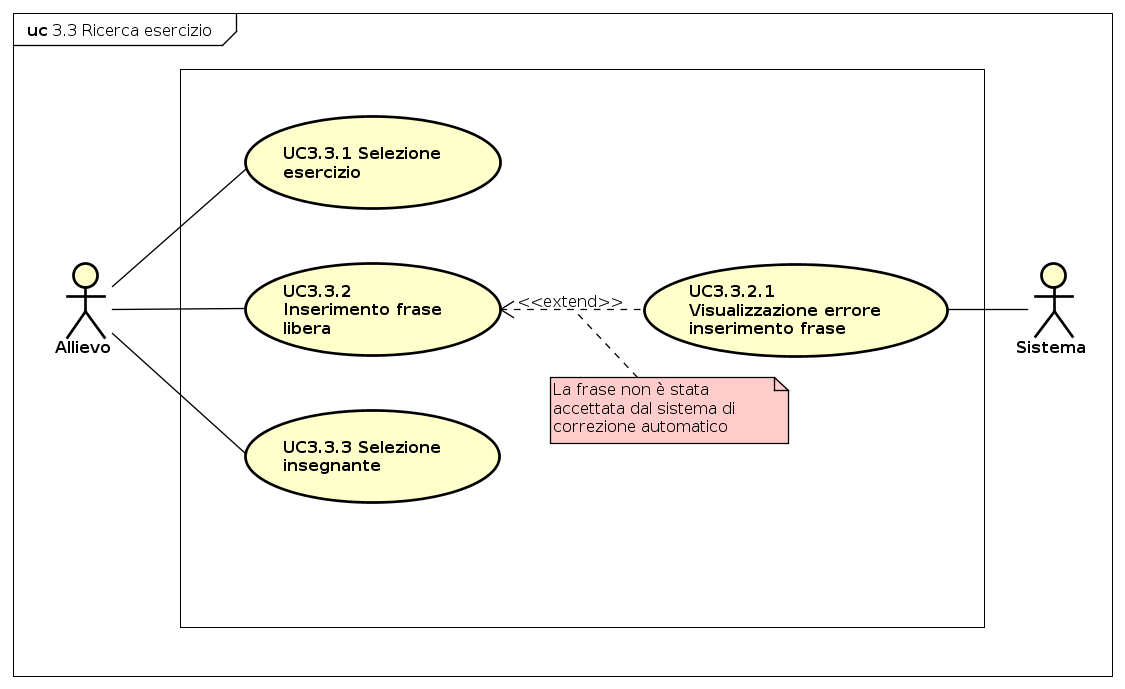
\includegraphics[scale=0.7]{img/UC33.png} 
\caption{Caso d'uso UC 3.3}
\end{figure}
\begin{itemize}
\item[•]\textbf{Attori}: Allievo;
\item[•]\textbf{Descrizione}: l'allievo visualizza i traguardi da lui raggiunti;
\item[•]\textbf{Precondizione}: l'allievo visualizza la propria dashboard;
\item[•]\textbf{Postcondizione}: l'allievo visualizza tutti i traguardi raggiunti;
\item[•]\textbf{Flusso degli eventi}: 
	\begin{itemize}
		\item[•] UC 3.3.1 - Visualizzazione prossimo traguardo;
		\item[•] UC 3.3.2 - Visualizzazione traguardo corrente.
	\end{itemize}
\end{itemize}

\subsubsection{UC 3.3.1 - Visualizzazione prossimo traguardo}
\begin{itemize}
\item[•]\textbf{Attori}: Allievo;
\item[•] \textbf{Descrizione}: l'allievo visualizza, nella propria dashboard, l'ammontare di punti mancante al raggiungimento del prossimo traguardo;
\item[•] \textbf{Precondizione}: l'allievo visualizza i propri traguardi;
\item[•] \textbf{Postcondizione}: l'allievo visualizza il punteggio mancante per raggiungere il traguardo successivo;
\item[•] \textbf{Flusso degli eventi}: l'allievo il punteggio mancante per il prossimo traguardo.
\end{itemize}

\subsubsection{UC 3.3.2 - Visualizzazione traguardo corrente}
\begin{itemize}
\item[•]\textbf{Attori}: Allievo;
\item[•] \textbf{Descrizione}: l'allievo visualizza, nella propria dashboard, il proprio traguardo personale raggiunto;
\item[•] \textbf{Precondizione}: l'allievo visualizza i propri traguardi;
\item[•] \textbf{Postcondizione}: l'allievo visualizza il traguardo corrente;
\item[•] \textbf{Flusso degli eventi}: l'allievo seleziona il traguardo corrente.
\end{itemize}


\subsubsection{UC 3.4 - Visualizzazione valutazioni}
\begin{itemize}
\item[•]\textbf{Attori}: Allievo;
\item[•]\textbf{Descrizione}: l'allievo visualizza le proprie valutazioni sugli esercizi;
\item[•]\textbf{Precondizione}: l'allievo visualizza la propria dashboard;
\item[•]\textbf{Postcondizione}: l'allievo visualizza tutte le valutazioni ricevute;
\item[•]\textbf{Flusso degli eventi}: l'allievo visualizza le valutazioni di tutti gli esercizi svolti, sia esercizi assegnati che svolti indipendentemente;
\item[•] \textbf{Flusso degli eventi alternativo}: 
	\begin{itemize}
		\item UC 3.4.1 - Visualizzazione valutazione esercizio		.
	\end{itemize}
\end{itemize}

\subsubsection{UC 3.4.1 - Visualizzazione valutazione esercizio}
\begin{itemize}
\item[•]\textbf{Attori}: Allievo;
\item[•]\textbf{Descrizione}: l'allievo visualizza la valutazione di un esercizio da lui precedentemente svolto;
\item[•]\textbf{Precondizione}: l'allievo sta visualizzando le sue valutazioni;
\item[•]\textbf{Postcondizione}: l'allievo visualizza il la valutazione dell'esercizio;
\item[•]\textbf{Flusso degli eventi}: l'allievo seleziona un esercizio specifico.
\end{itemize}

\subsubsection{UC 3.5 - Inserimento insegnante preferito}
\begin{itemize}
\item[•]\textbf{Attori}: Allievo;
\item[•]\textbf{Descrizione}: l'allievo inserisce un nuovo insegnante preferito;
\item[•]\textbf{Precondizione}: l'allievo visualizza la propria dashboard;
\item[•]\textbf{Postcondizione}: l'allievo ha inserito un insegnante preferito;
\item[•]\textbf{Flusso degli eventi}: l'allievo inserisce il nominativo di un insegnante da prediligere quando riceve la correzione di un esercizio.
\end{itemize}

\subsubsection{UC 3.6 - Visualizzazione insegnanti preferiti}
\begin{itemize}
	\item[•]\textbf{Attori}: Allievo;
	\item[•]\textbf{Descrizione}: l'allievo visualizza la lista degli insegnanti preferiti;
	\item[•]\textbf{Precondizione}: l'allievo visualizza la propria dashboard;
	\item[•]\textbf{Postcondizione}: l'allievo visualizza gli insegnanti preferiti.
	\item[•]\textbf{Flusso degli eventi}: l'allievo visualizza la lista degli insegnanti preferiti che ha precedentemente inserito.
\end{itemize}

\subsubsection{UC 3.7 - Rimozione insegnante preferito}
\begin{itemize}
	\item[•]\textbf{Attori}: Allievo;
	\item[•]\textbf{Descrizione}: l'allievo rimuove un insegnante preferito;
	\item[•]\textbf{Precondizione}: l'allievo visualizza la lista di insegnanti preferiti;
	\item[•]\textbf{Postcondizione}: l'allievo ha rimosso un insegnante preferito dalla lista;
	\item[•]\textbf{Flusso degli eventi}: 
	\begin{enumerate}
	 \item Seleziona insegnante dalla lista;
	 \item Elimina insegnante selezionato.
	\end{enumerate}
\end{itemize}

\subsubsection{UC 3.8 - Selezione lingua esercizi}
\begin{itemize}
	\item[•]\textbf{Attori}: Allievo;
	\item[•]\textbf{Descrizione}: l'allievo seleziona la lingua in cui vuole svolgere gli esercizi;
	\item[•]\textbf{Precondizione}: l'allievo visualizza la propria dashboard;
	\item[•]\textbf{Postcondizione}: l'allievo ha selezionato una lingua per gli esercizi;
	\item[•]\textbf{Flusso degli eventi}: l'allievo seleziona da un elenco predefinito la lingua degli esercizi.
\end{itemize}

\subsubsection{UC 3.9 - Visualizzazione elenco esercizi}
\begin{itemize}
\item[•]\textbf{Attori}: Allievo;
\item[•]\textbf{Descrizione}:  l'allievo visualizza un elenco di frasi consigliate dal sistema come esercizi oppure gli esercizi assegnati dall'insegnante;
\item[•]\textbf{Precondizione}: l'allievo visualizza la propria dashboard;
\item[•]\textbf{Postcondizione}: l'allievo visualizza un elenco di esercizi;
\item[•]\textbf{Flusso degli eventi}: l'allievo seleziona la sezione riguardante gli esercizi che possono essere da lui svolti.
\end{itemize}

\subsubsection{UC 3.10 - Esercitazione libera}
\begin{figure}[H]
	\centering
	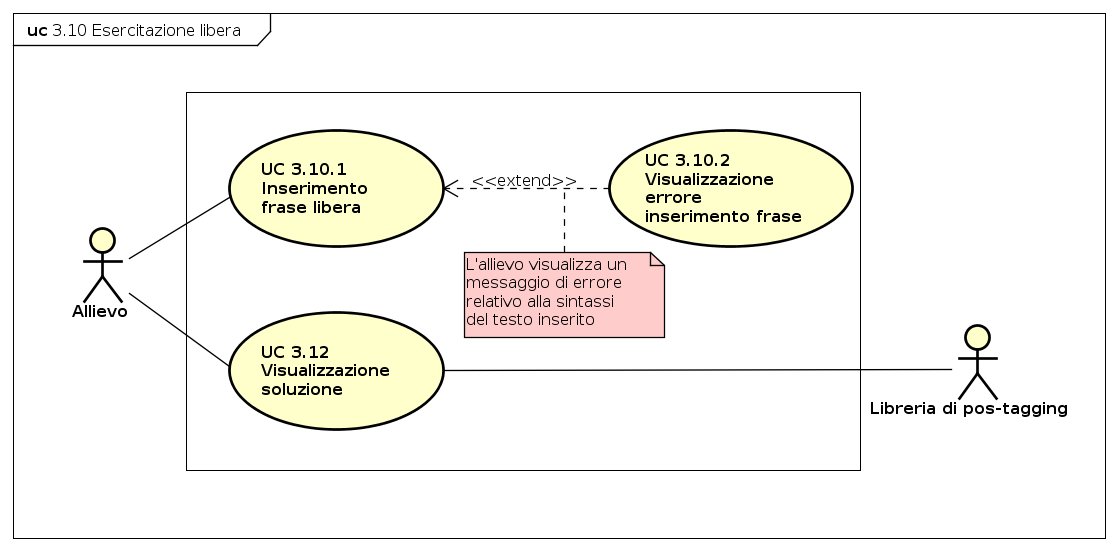
\includegraphics[width=17cm]{img/UC310.png} 
	\caption{Caso d'uso 3.10}\label{fig:310}
\end{figure}
\begin{itemize}
\item[•]\textbf{Attori}: Allievo;
\item[•]\textbf{Descrizione}: l'allievo inserisce liberamente una frase in modo da riceverne l'analisi grammaticale;
\item[•]\textbf{Precondizione}: l'allievo visualizza la propria dashboard;
\item[•]\textbf{Postcondizione}: l'allievo ha visualizzato l'analisi grammaticale della frase inserita.
\item[•]\textbf{Flusso degli eventi}:
\begin{enumerate}
	\item UC 3.10.1 - Inserimento frase libera;
	\item UC 3.10.3 - Visualizzazione analisi automatica.
\end{enumerate}
\end{itemize}

\subsubsection{UC 3.10.1 - Inserimento frase libera}
\begin{itemize}
	\item[•]\textbf{Attori}: Allievo;
	\item[•]\textbf{Descrizione}: l'allievo può inserire una frase libera da svolgere;
	\item[•]\textbf{Precondizione}: l'allievo si è autenticato;
	\item[•]\textbf{Postcondizione}: l'allievo ha inserito una frase;
	\item[•]\textbf{Flusso degli eventi}: l'allievo inserisce una frase libera da svolgere autonomamente per poi ricevere una valutazione automatica;
	\item[•]\textbf{Estensioni}:
	\begin{enumerate}
		\item UC 3.10.2 - Visualizzazione errore inserimento frase.
	\end{enumerate}
\end{itemize}

\subsubsection{UC 3.10.2 - Visualizzazione errore inserimento frase}
\begin{itemize}
	\item[•]\textbf{Attori}: Allievo;
	\item[•]\textbf{Descrizione}: l'allievo visualizza un messaggio di errore durante l'inserimento di una frase;
	\item[•]\textbf{Precondizione}: l'allievo ha inserito una frase;
	\item[•]\textbf{Postcondizione}: l'allievo ha visualizzato il messaggio di errore e può inserire una nuova frase;
	\item[•]\textbf{Flusso degli eventi}: durante l'inserimento di una frase libera nel sistema tale frase non viene accettata, viene visualizzato un errore.
\end{itemize}

\subsubsection{UC 3.10.3 - Visualizzazione analisi automatica}
\begin{itemize}
	\item[•]\textbf{Attori}: Allievo, Libreria di pos-tagging;
	\item[•]\textbf{Descrizione}: l'allievo visualizza l'analisi grammaticale della frase inserita;
	\item[•]\textbf{Precondizione}: l'allievo ha inserito una frase libera;
	\item[•]\textbf{Postcondizione}: l'allievo visualizza l'analisi grammaticale della frase inserita;
	\item[•]\textbf{Flusso degli eventi}: l'allievo ha richiesto l'analisi automatica della frase da lui inserita.
\end{itemize}

\subsubsection{UC 3.11 - Svolgimento esercizio}
\begin{figure}[H]
	\centering
	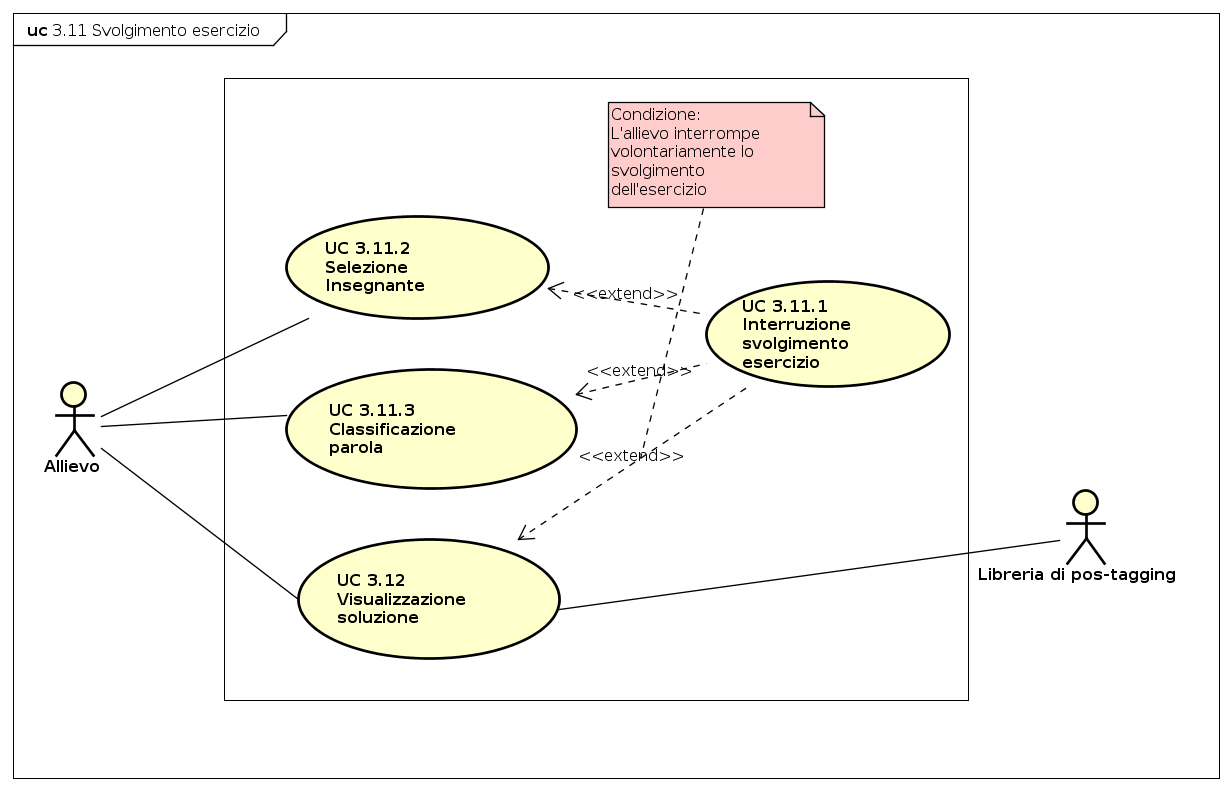
\includegraphics[width=17cm]{img/UC311.png} 
	\caption{Caso d'uso 3.11}\label{fig:311}
\end{figure}
\begin{itemize}
	\item[•]\textbf{Attori}: Allievo;
	\item[•]\textbf{Descrizione}: l'allievo può svolgere l'esercizio scegliendo le classi grammaticali per ciascuna parola da un' apposita lista;
	\item[•]\textbf{Precondizione}: l'allievo ha selezionato un esercizio;
	\item[•]\textbf{Postcondizione}: l'allievo ha svolto un esercizio;
	\item[•]\textbf{Flusso degli eventi}:
	\begin{enumerate}
		\item Selezione esercizio;
		\item UC 3.11.3 - Classificazione parola;
		\item UC 3.12 - Visualizzazione soluzione.
	\end{enumerate}
	\item[•]\textbf{Estensioni}:
	\begin{enumerate}
		\item UC 3.11.1 - Interruzione svolgimento esercizio;
	\end{enumerate}
	\item[•] \textbf{Flusso alternativo}:
	\begin{itemize}
				\item UC 3.11.2 - Selezione insegnante.
	\end{itemize}
\end{itemize}

\subsubsection{UC 3.11.1 - Interruzione svolgimento esercizio}
\begin{itemize}
	\item[•]\textbf{Attori}: Allievo;
	\item[•]\textbf{Descrizione}: l'allievo interrompe lo svolgimento di un esercizio;
	\item[•]\textbf{Precondizione}: l'allievo inizia a svolgere un esercizio;
	\item[•]\textbf{Postcondizione}: l'allievo interrompe l'esercizio, torna nella sezione di visualizzazione elenco esercizi;
	\item[•]\textbf{Flusso degli eventi}: durante lo svolgimento di un esercizio l'allievo lo interrompe, scartando i dati inseriti fino a quel momento, e ritorna nella sezione di visualizzazione elenco esercizi.
\end{itemize}

\subsubsection{UC 3.11.2 - Selezione insegnante}
\begin{itemize}
	\item[•]\textbf{Attori}: Allievo;
	\item[•]\textbf{Descrizione}: l'allievo seleziona l'insegnante da cui vuole ricevere la correzione, se nessun insegnante ha predisposto quella frase verrà utilizzato il sistema di correzione automatico;
	\item[•]\textbf{Precondizione}: l'allievo ha selezionato un esercizio;
	\item[•]\textbf{Postcondizione}: l'allievo seleziona l'insegnante dal quale vuole ricevere la correzione;
	\item[•]\textbf{Flusso degli eventi}: durante lo svolgimento di un esercizio  l'allievo seleziona l'insegnante da cui vuole ricevere la correzione dell'esercizio.
\end{itemize}

\subsubsection{UC 3.11.3 - Classificazione parola}
\begin{itemize}
	\item[•]\textbf{Attori}: Allievo;
	\item[•]\textbf{Descrizione}: l'allievo assegna una classe grammaticale ad una parola;
		\item[•]\textbf{Precondizione}: l'allievo sta svolgendo un esercizio.
	\item[•]\textbf{Postcondizione}: l'allievo seleziona la classe grammaticale di una parola.
	\item[•]\textbf{Flusso degli eventi}: durante lo svolgimento di un esercizio  l'allievo seleziona i tag da una lista predefinita: nome, pronome, articolo, aggettivo, verbo, preposizione, congiunzione, avverbio ed esclamazione.
\end{itemize}


\subsubsection{UC 3.12 - Visualizzazione soluzione}
\begin{figure}[H]
	\centering
	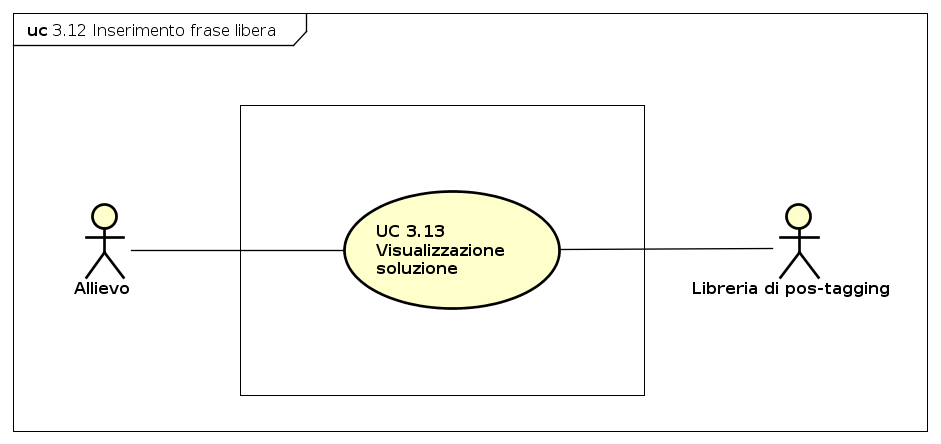
\includegraphics[width=17cm]{img/UC312.png} 
	\caption{Caso d'uso UC 3.12}\label{fig:312}
\end{figure}
\begin{itemize}
	\item[•]\textbf{Attori}: Allievo;
	\item[•]\textbf{Descrizione}: l'allievo visualizza la correzione secondo l'insegnante selezionato in precedenza;
	\item[•]\textbf{Precondizione}: l'allievo ha svolto un esercizio;
	\item[•]\textbf{Postcondizione}: l'allievo visualizza la soluzione dell'esercizio;
	\item[•]\textbf{Flusso degli eventi}:
	\begin{enumerate}
		\item UC 3.12.1 - Visualizzazione valutazione esercizio.  
	\end{enumerate}
\end{itemize}


\subsubsection{UC 3.12.1 - Visualizzazione valutazione esercizio}   

\begin{itemize}
\item[•]\textbf{Attori}: Allievo;
\item[•]\textbf{Descrizione}:  l'allievo riceve una valutazione di un esercizio svolto;
\item[•]\textbf{Precondizione}: l'allievo visualizza la soluzione dell'esercizio svolto;
\item[•]\textbf{Postcondizione}: l'allievo visualizza una valutazione sull'esercizio svolto;
\item[•]\textbf{Flusso degli eventi}: l'allievo ha ri
\end{itemize}

\subsubsection{UC 3.13 - Modifica dati utente}
\begin{figure}[H]
	\centering
	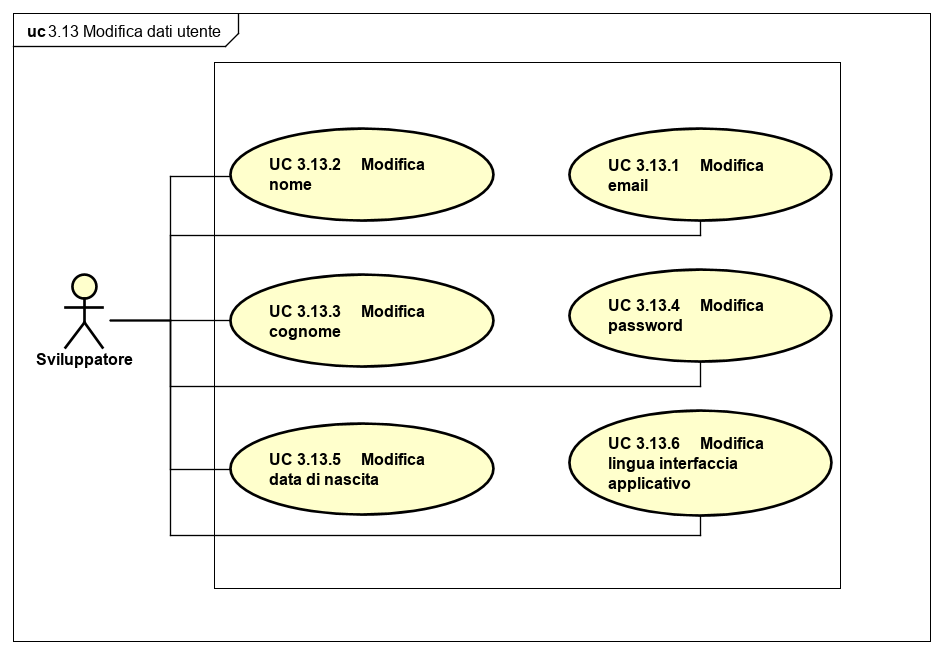
\includegraphics[width=13cm]{img/modificadatiutenteallievo.png} 
	\caption{Caso d'uso UC 3.13}\label{fig:312}
\end{figure}
\begin{itemize}
\item[•] \textbf{Attori}: Allievo;
\item[•] \textbf{Descrizione}: l'allievo modifica i propri dati personali, cioè tutti i dati personali inseriti in fase di registrazione;
\item[•] \textbf{Precondizione}: l'allievo visualizza la propria dashboard;
\item[•] \textbf{Postcondizione}: l'allievo ha modificato uno o più dati personali;
\item[•] \textbf{Flusso degli eventi}:
\begin{enumerate}
	\item[•] Selezione procedura modifica dati personali;
	\item[•] UC 3.13.1 - Modifica email;
	\item[•] UC 3.13.2 - Modifica nome;
	\item[•] UC 3.13.3 - Modifica cognome;
	\item[•] UC 3.13.4 - Modifica password;
	\item[•] UC 3.13.5 - Modifica data di nascita;
	\item[•] UC 3.13.6 - Modifica lingua
	 interfaccia applicativo;
\end{enumerate}
\end{itemize}


\subsubsection{UC 3.13.1 - Modifica email}
\begin{itemize}
	\item[•]\textbf{Attori}: Allievo;
	\item[•]\textbf{Descrizione}: l'allievo modifica la propria email;
	\item[•]\textbf{Precondizione}: l'allievo sta modificando i propri dati personali;
	\item[•]\textbf{Postcondizione}: l'allievo ha modificato la propria email; 
	\item[•]\textbf{Flusso degli eventi}: 
	\begin{enumerate}
		\item Selezione campo email;
		\item Modifica la stringa che rappresenta la propria email.
	\end{enumerate}
\end{itemize}
\subsubsection{UC 3.13.2 - Modifica nome}
\begin{itemize}
	\item[•]\textbf{Attori}: Allievo;
	\item[•]\textbf{Descrizione}: l'allievo modifica il proprio nome;
	\item[•]\textbf{Precondizione}: l'allievo sta modificando i propri dati personali;
	\item[•]\textbf{Postcondizione}: l'allievo ha modificato il proprio nome; 
	\item[•]\textbf{Flusso degli eventi}: 
	\begin{enumerate}
		\item Selezione campo nome;
		\item Modifica la stringa che rappresenta il nome.
	\end{enumerate}
\end{itemize}
\subsubsection{UC 3.13.3 - Modifica cognome}
\begin{itemize}
	\item[•]\textbf{Attori}: Allievo;
	\item[•]\textbf{Descrizione}: l'allievo modifica il proprio cognome;
	\item[•]\textbf{Precondizione}: l'allievo sta modificando i propri dati personali;
	\item[•]\textbf{Postcondizione}: l'allievo ha modificato il proprio cognome; 
	\item[•]\textbf{Flusso degli eventi}: 
	\begin{enumerate}
		\item Selezione campo cognome;
		\item Modifica la stringa che rappresenta il cognome.
	\end{enumerate}
\end{itemize}
\subsubsection{UC 3.13.4 - Modifica password}
\begin{figure}[H]
	\centering
	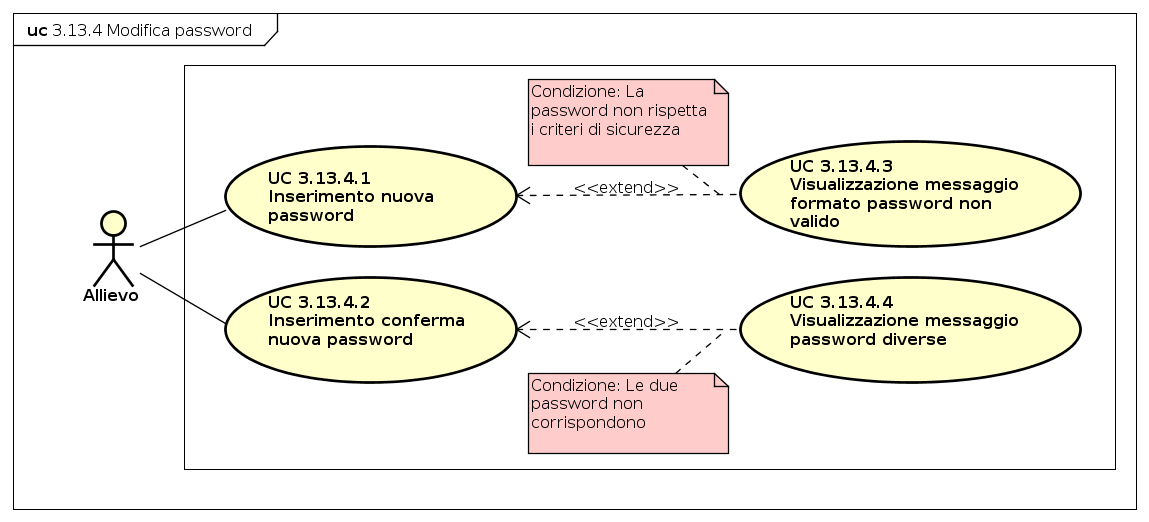
\includegraphics[width=15cm, keepaspectratio]{img/UC3134.png} 
	\caption{Caso d'uso UC 3.13.4}\label{fig:3134}
\end{figure}
\begin{itemize}
	\item[•]\textbf{Attori}: Allievo;
	\item[•]\textbf{Descrizione}: l'allievo modifica la propria password;
	\item[•]\textbf{Precondizione}: l'allievo sta modificando i la propria password personale;
	\item[•]\textbf{Postcondizione}: l'allievo ha modificato la propria password personale; 
	\item[•]\textbf{Flusso degli eventi}: 
	\begin{enumerate}
		\item UC 3.13.4.1 - Inserimento nuova password;
		\item UC 3.13.4.2 - Inserimento conferma nuova password.
	\end{enumerate}
\end{itemize}
\subsubsection{UC 3.13.5 - Modifica data di nascita}
\begin{itemize}
	\item[•]\textbf{Attori}: Allievo;
	\item[•]\textbf{Descrizione}: l'allievo modifica il proprio cognome;
	\item[•]\textbf{Precondizione}: l'allievo sta modificando i propri dati personali;
	\item[•]\textbf{Postcondizione}: l'allievo ha modificato il proprio cognome; 
	\item[•]\textbf{Flusso degli eventi}: 
	\begin{enumerate}
		\item Selezione campo data di nascita;
		\item Modifica la stringa che rappresenta la data di nascita, inserendo il valore corretto.
	\end{enumerate}
\end{itemize}
\subsubsection{UC 3.13.6 - Modifica lingua interfaccia applicativo}
\begin{itemize}
	\item[•]\textbf{Attori}: Allievo;
	\item[•]\textbf{Descrizione}: lo sviluppatore modifica la lingua dell'applicativo;
	\item[•]\textbf{Precondizione}: lo sviluppatore sta modificando i propri dati personali;
	\item[•]\textbf{Postcondizione}: lo sviluppatore ha modificato la lingua dell'applicativo; 
	\item[•]\textbf{Flusso degli eventi}: 
	\begin{enumerate}
		\item Selezione campo dati lingua applicativo;
		\item Selezione da un elenco predefinito la lingua dell'applicativo desiderata.
	\end{enumerate}
\end{itemize}

\subsubsection{UC 3.13.4.1 - Inserimento nuova password}
\begin{itemize}
	\item[•]\textbf{Attori}: Allievo;
	\item[•]\textbf{Descrizione}: l'allievo inserisce la nuova password;
	\item[•]\textbf{Precondizione}: l'allievo sta modificando i propri dati personali;
	\item[•]\textbf{Postcondizione}: l'allievo ha inserito il valore della nuova password; 
	\item[•]\textbf{Flusso degli eventi}: 
	\begin{enumerate}
		\item Selezione campo dati relativo alla nuova password;
		\item Inserimento stringa rappresentante la password.
	\end{enumerate}
	\item[•]\textbf{Estensioni}:
	\begin{enumerate}
		\item UC 3.13.4.3 - Visualizzazione messaggio formato password non valido.
	\end{enumerate}
\end{itemize}

\subsubsection{UC 3.13.4.2 - Inserimento conferma nuova password}
\begin{itemize}
	\item[•]\textbf{Attori}: Allievo;
	\item[•]\textbf{Descrizione}: l'allievo inserisce conferma la nuova password, reinserendola nell'apposito campo;
	\item[•]\textbf{Precondizione}: l'allievo sta modificando i propri dati personali;
	\item[•]\textbf{Postcondizione}: l'allievo ha inserito il valore del campo conferma nuova password; 
	\item[•]\textbf{Flusso degli eventi}: 
	\begin{enumerate}
		\item Selezione campo dati relativo alla conferma nuova password;
		\item Inserimento stringa rappresentante la password.
	\end{enumerate}
	\item[•]\textbf{Estensioni}:
	\begin{enumerate}
		\item UC 3.13.4.4 - Visualizzazione messaggio password diverse.
	\end{enumerate}
\end{itemize}

\subsubsection{UC 3.13.4.3 - Visualizzazione messaggio formato password non valido}
\begin{itemize}
	\item[•]\textbf{Attori}: Allievo;
	\item[•]\textbf{Descrizione}: l'allievo ha inserito una password con un formato non valido;
	\item[•]\textbf{Precondizione}: l'allievo sta modificando i propri dati personali;
	\item[•]\textbf{Postcondizione}: l'allievo visualizza un messaggio di errore relativo all'inserimento di una password che non rispetta un formato valido; 
	\item[•]\textbf{Flusso degli eventi}: l'allievo ha inserito una password che non rispetta i criteri accettati dal sistema, pertanto riceve un messaggio che indica la presenza di un formato non adatto.
\end{itemize}

\subsubsection{UC 3.13.4.4 - Visualizzazione messaggio password diverse}
\begin{itemize}
	\item[•]\textbf{Attori}: Allievo;
	\item[•]\textbf{Descrizione}: l' allievo ha inserito un valore di conferma password che non corrisponde al valore della nuova password inserita precedentemente, pertanto visualizza un messaggio che indica che le due password non corrispondono;
	\item[•]\textbf{Precondizione}: l'allievo ha inserito il valore del campo conferma nuova password;
	\item[•]\textbf{Postcondizione}: l'allievo visualizza un messaggio di errore relativo all'inserimento di una password che non combacia con quella inserita nel campo nuova password; 
	\item[•]\textbf{Flusso degli eventi}: l'allievo ha inserito una password che non combacia con quella inserita nel campo nuova password, pertanto riceve un messaggio che indica la presenza di tale difformità.
\end{itemize}

\subsubsection{UC 3.14 - Logout}
\begin{itemize}
    \item[•] \textbf{Attori}: Allievo;
    \item[•] \textbf{Descrizione}: l'allievo effettua il logout dal sistema;
    \item[•] \textbf{Precondizione}: l'allievo si è autenticato;
    \item[•] \textbf{Postcondizione}: l'allievo effettua il logout dal sistema e viene reindirizzato alla pagina di login;
    \item[•] \textbf{Flusso degli eventi}: l'allievo seleziona il bottone di logout e esce dalla sessione.
\end{itemize}
\newpage
\subsection{Sviluppatori}
\subsubsection{Panoramica sviluppatore}
\begin{figure}[H]
	\centering
	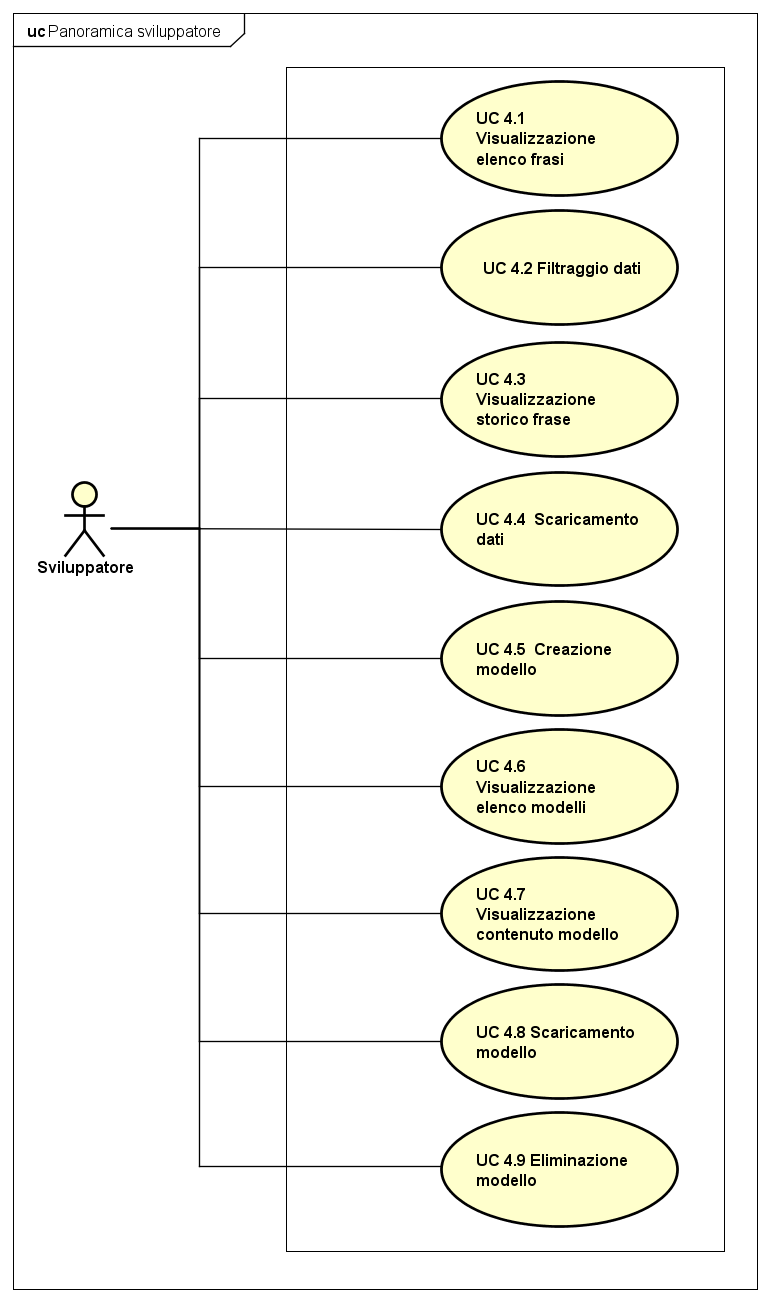
\includegraphics[width=17cm, keepaspectratio]{img/UC4x.png} 
	\caption{Panoramica sviluppatore}\label{fig:4x}
\end{figure}
\subsubsection{UC 4.1 - Visualizzazione dashboard}
\begin{itemize}
	\item[•]\textbf{Attori}: Sviluppatore;
	\item[•]\textbf{Descrizione}: lo sviluppatore ha effettuato l'autenticazione e visualizza la propria dashboard, la quale gli permette di accedere alle seguenti operazioni: creare e eliminare i modelli, visualizzare lo storico delle frasi inserite e modificare i propri dati personali;
	\item[•]\textbf{Precondizione}: lo sviluppatore ha effettuato l'autenticazione;
	\item[•]\textbf{Postcondizione}: lo sviluppatore visualizza la propria dashboard; 
	\item[•]\textbf{Flusso degli eventi}: lo sviluppatore ha effettuato l'autenticazione e viene automaticamente reindirizzato alla pagina che contiene la dashboard.
\end{itemize}
\subsubsection{UC 4.2 - Visualizzazione elenco frasi}
\begin{itemize}
	\item[•]\textbf{Attori}: Sviluppatore;
	\item[•]\textbf{Descrizione}: lo sviluppatore visualizza un elenco di frasi accompagnate 
	dalla data di creazione e dall’autore ordinate cronologicamente;
	\item[•]\textbf{Precondizione}:  lo sviluppatore si è autenticato nel sistema e visualizza la propria dashboard;
	\item[•]\textbf{Postcondizione}: lo sviluppatore visualizza l'elenco delle preposizioni ordinate cronologicamente comprensive di analisi grammaticale, data, autore e livello di attendibilità;
	\item[•]\textbf{Flusso degli eventi}: lo sviluppatore ha selezionato la voce relativa alla pagina contenente l’elenco delle frasi e ne visualizza il contenuto. 
\end{itemize}
\subsubsection{UC 4.3 - Filtraggio dei dati}
\begin{figure}[H]
	\centering
	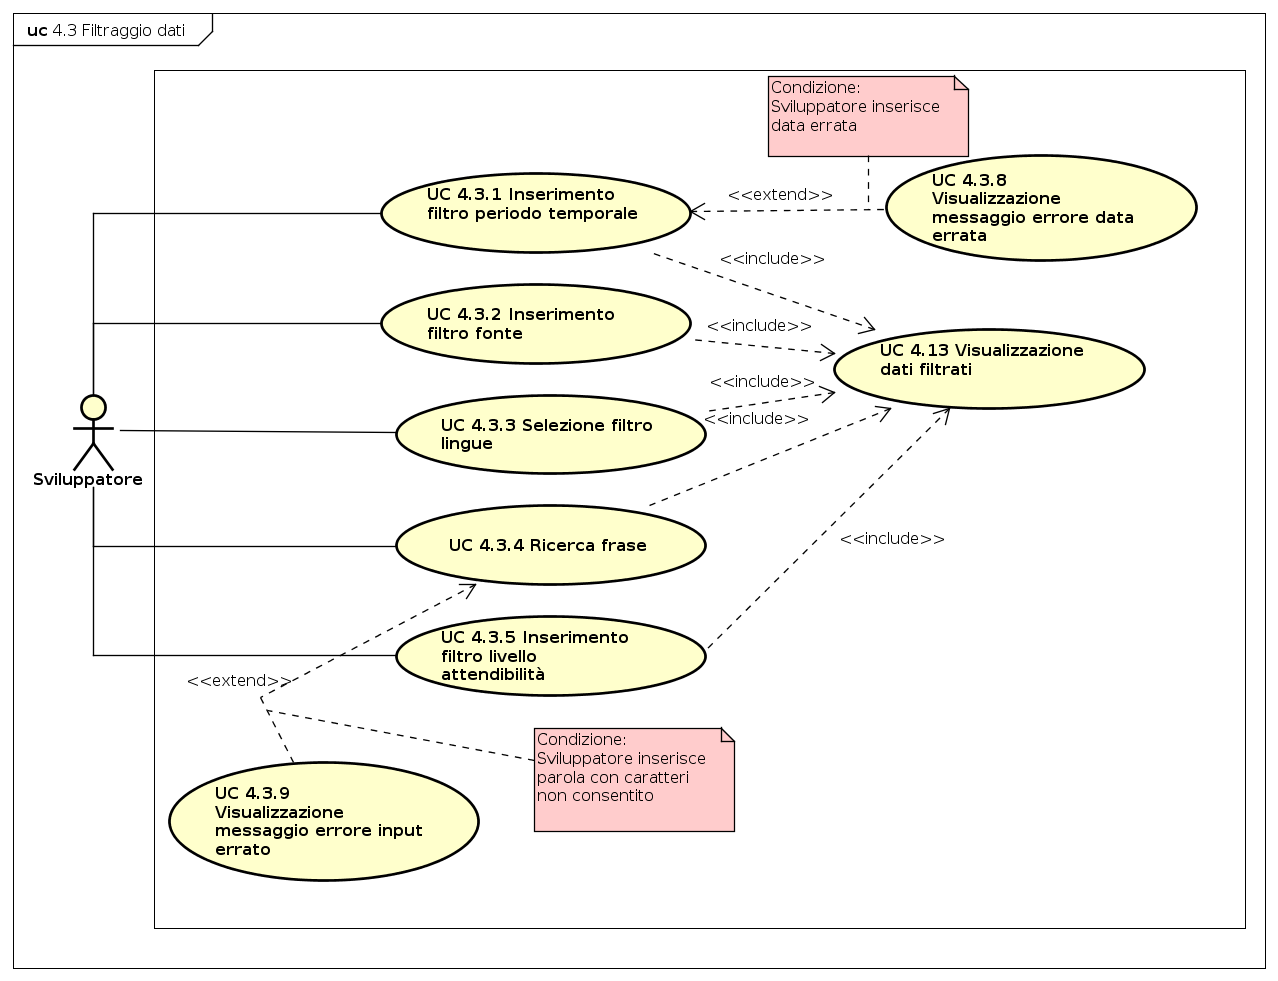
\includegraphics[width=14cm, keepaspectratio]{img/UC430.png} 
	\caption{Caso d'uso UC 4.3}\label{fig:430}
\end{figure}
\begin{itemize}
	\item[•]\textbf{Attori}: Sviluppatore;
	\item[•]\textbf{Descrizione}: lo sviluppatore applica dei filtri ai dati, ottenendo solo quelli d'interesse;
	\item[•]\textbf{Precondizione}: lo sviluppatore visualizza le proposizioni in ordine cronologico (UC 4.2);
	\item[•]\textbf{Postcondizione}: lo sviluppatore visualizza i dati che rispettano i filtri scelti;
	\item[•]\textbf{Flusso degli eventi}:
	\begin{enumerate}
		\item UC 4.3.1 - Inserimento filtro periodo temporale;
		\item UC 4.3.2 - Inserimento filtro {fonte}\ped{G};
		\item UC 4.3.3 - Selezione filtro lingue;
		\item UC 4.3.4 - Ricerca parole chiave;
		\item UC 4.3.5 - Inserimento filtro livello attendibilità.
	\end{enumerate}
	\item[•]\textbf{Estensioni}:
	\begin{enumerate}
%		\item UC 4.3.7 - Rimozione filtro;
		\item UC 4.3.7 - Visualizzazione messaggio errore data errata;
		\item UC 4.3.8 - Visualizzazione messaggio errore input errato.
	\end{enumerate}
	\item[•]\textbf{Inclusioni}:
	\begin{enumerate}
		\item UC 4.13 - Visualizzazione dati filtrati.
	\end{enumerate}
\end{itemize}
\subsubsection{UC 4.3.1 - Inserimento filtro periodo temporale}
\begin{itemize}
	\item[•]\textbf{Attori}: Sviluppatore;
	\item[•]\textbf{Descrizione}: lo sviluppatore seleziona un periodo temporale, ottenendo i dati salvati in un determinato arco di tempo;
	\item[•]\textbf{Precondizione}: lo sviluppatore visualizza le proposizioni in base ai filtri stabiliti;
	\item[•]\textbf{Postcondizione}: lo sviluppatore visualizza le frasi che rispettano il periodo di tempo indicato nel filtro;
	\item[•]\textbf{Flusso degli eventi}: 
	\begin{enumerate}
		\item Scelta data inizio periodo;
		\item Scelta data fine periodo.
	\end{enumerate}
	\item[•]\textbf{Estensioni}: 
	\begin{enumerate}
%		\item UC 4.3.7 - Rimozione filtro;
		\item UC 4.3.7 - Visualizzazione messaggio errore data errata.
	\end{enumerate}
	\item[•]\textbf{Inclusioni}:
	\begin{enumerate}
		\item UC 4.13 - Visualizzazione dati filtrati.
	\end{enumerate}
\end{itemize}

\subsubsection{UC 4.3.2 - Inserimento filtro fonte}
\begin{itemize}
	\item[•]\textbf{Attori}: Sviluppatore;
	\item[•]\textbf{Descrizione}: lo sviluppatore seleziona una o più fonti degli esercizi, come ad esempio le correzione provenienti da determinati docenti o dal sistema di correzione automatico;
	\item[•]\textbf{Precondizione}: lo sviluppatore visualizza le proposizioni in base ai filtri stabiliti;
	\item[•]\textbf{Postcondizione}: lo sviluppatore ha impostato i valori del filtro fonte, pertanto vuole visualizzare tutte le proposizioni inserite da una determinata fonte ed eventualmente gli altri filtri;
	\item[•]\textbf{Flusso degli eventi}: lo sviluppatore seleziona da un elenco le fonti di cui è interessato visualizzare i dati;
%	\item[•]\textbf{Estensioni}: 
%	\begin{enumerate}
%		\item UC 4.3.7 - Rimozione filtro.
%	\end{enumerate}
	\item[•]\textbf{Inclusioni}:
	\begin{enumerate}
		\item UC 4.13 - Visualizzazione dati filtrati.
	\end{enumerate}
\end{itemize}

\subsubsection{UC 4.3.3 -  Selezione filtro lingue}
\begin{itemize}
	\item[•]\textbf{Attori}: Sviluppatore;
	\item[•]\textbf{Descrizione}: lo sviluppatore seleziona una o più lingue da un elenco di lingue predefinito al fine di ottenere solamente le proposizioni scritte in tali lingue;
	\item[•]\textbf{Precondizione}: lo sviluppatore visualizza le proposizioni in base ai filtri stabiliti;
	\item[•]\textbf{Postcondizione}: lo sviluppatore ha stabilito i valori di filtraggio relativi alle lingue, quindi visualizza tutte le frasi scritte in tale lingua e che soddisfano anche gli altri filtri applicati;
	\item[•]\textbf{Flusso degli eventi}: lo sviluppatore seleziona da un elenco le lingue di cui è interessato vedere le proposizioni memorizzate;
%	\item[•]\textbf{Estensioni}: 
%	\begin{enumerate}
%		\item UC 4.3.7 - Rimozione filtro.
%	\end{enumerate}
	\item[•]\textbf{Inclusioni}:
	\begin{enumerate}
		\item UC 4.13 - Visualizzazione dati filtrati.
	\end{enumerate}
\end{itemize}

\subsubsection{UC 4.3.4 - Ricerca frase}
\begin{itemize}
	\item[•]\textbf{Attori}: Sviluppatore;
	\item[•]\textbf{Descrizione}: lo sviluppatore scrive una o più parole chiave al fine di cernere le frasi contenenti tali parole;
	\item[•]\textbf{Precondizione}: lo sviluppatore visualizza le frasi in base al filtraggio scelto;
	\item[•]\textbf{Postcondizione}: lo sviluppatore ha impostato le parole chiave e visualizza solamente le frasi che contengono solamente quelle parole e che rispettano gli altri filtri inseriti;
	\item[•]\textbf{Flusso degli eventi}: lo sviluppatore inserisce una stringa rappresentate una o più parole chiave che devono essere contenute nelle stringhe che intende visualizzare;
	\item[•]\textbf{Estensioni}: 
	\begin{enumerate}
%		\item UC 4.3.7 - Rimozione filtro;
		\item UC 4.3.8 - Visualizzazione messaggio di errore input errato.
	\end{enumerate}
	\item[•]\textbf{Inclusioni}:
	\begin{enumerate}
		\item UC 4.13 - Visualizzazione dati filtrati.
	\end{enumerate}
\end{itemize}

\subsubsection{UC 4.3.5 - Inserimento filtro livello attendibilità}
\begin{itemize}
	\item[•]\textbf{Attori}: Sviluppatore;
	\item[•]\textbf{Descrizione}: lo sviluppatore seleziona un valore numerico rappresentante il livello di attendibilità delle frasi che vuole visualizzare, ovvero frasi le cui correzioni sono uguali a quelle di altre insegnanti acquisiscono un livello di attendibilità maggiore rispetto ad altre;
	\item[•]\textbf{Precondizione}: i valori di uno o più filtri sono stati inseriti;
	\item[•]\textbf{Postcondizione}: lo sviluppatore ha selezionato il livello di attendibilità e visualizza solamente le frasi che hanno tale livello di attendibilità, cioè che hanno ricevuto la stessa correzione da più insegnanti, e che rispettano eventualmente gli altri filtri inseriti;
	\item[•]\textbf{Flusso degli eventi}: lo sviluppatore seleziona da un elenco predefinito il livello di attendibilità desiderato;
%\item[•]\textbf{Estensioni}: 
%	\begin{enumerate}
%		\item UC 4.3.7 - Rimozione filtro.
%	\end{enumerate}
	\item[•]\textbf{Inclusioni}:
	\begin{enumerate}
		\item UC 4.13 - Visualizzazione dati filtrati.
	\end{enumerate}
\end{itemize}



\subsubsection{UC 4.3.7 - Visualizzazione messaggio errore data errata}
\begin{itemize}
	\item[•]\textbf{Attori}: Sviluppatore;
	\item[•]\textbf{Descrizione}: lo sviluppatore visualizza un messaggio di errore sul periodo selezionato;
	\item[•]\textbf{Precondizione}: lo sviluppatore ha inserito una data non conforme all'interno del filtro relativo al periodo temporale;
	\item[•]\textbf{Postcondizione}: il filtro è stato erroneamente inserito pertanto viene visualizzato un messaggio di errore;
	\item[•]\textbf{Flusso degli eventi}: lo sviluppatore ha inserito una data non conforme, cioè che non rispetta il formato stabilito o che indica un periodo temporale non idoneo, pertanto visualizza un messaggio di errore.
\end{itemize}

\subsubsection{UC 4.3.8 - Visualizzazione messaggio errore input errato}
\begin{itemize}
	\item[•]\textbf{Attori}: Sviluppatore;
	\item[•]\textbf{Descrizione}: lo sviluppatore visualizza un messaggio di errore sulla ricerca;
	\item[•]\textbf{Precondizione}: lo sviluppatore ha inserito una frase non conforme;
	\item[•]\textbf{Postcondizione}: lo sviluppatore visualizza un messaggio di errore relativo 
	all'inserimento di un input errato, cioè non conforme a ciò che il sistema si attendeva;
	\item[•]\textbf{Flusso degli eventi}: lo sviluppatore inserisce un input non conforme, cioè contenente caratteri non ammessi, e visualizza un messaggio di input errato.
\end{itemize}

\subsubsection{UC 4.4 - Visualizzazione storico frase}
\begin{itemize}
	\item[•]\textbf{Attori}: Sviluppatore;
	\item[•]\textbf{Descrizione}: lo sviluppatore seleziona una frase dall'elenco e ne visualizza lo storico contenente la correzione fornita dal sistema automatico, ed eventualmente quelle redatte anche da insegnanti diversi;
	\item[•]\textbf{Precondizione}: lo sviluppatore visualizza le frasi in base ai filtri stabiliti;
	\item[•]\textbf{Postcondizione}: lo sviluppatore visualizza tutte le correzioni della frase;
	\item[•]\textbf{Flusso degli eventi}: lo sviluppatore seleziona la frase e appare lo storico della frase.
\end{itemize}

\subsubsection{UC 4.5 - Scaricamento dati}
\begin{figure}[H]
	\centering
	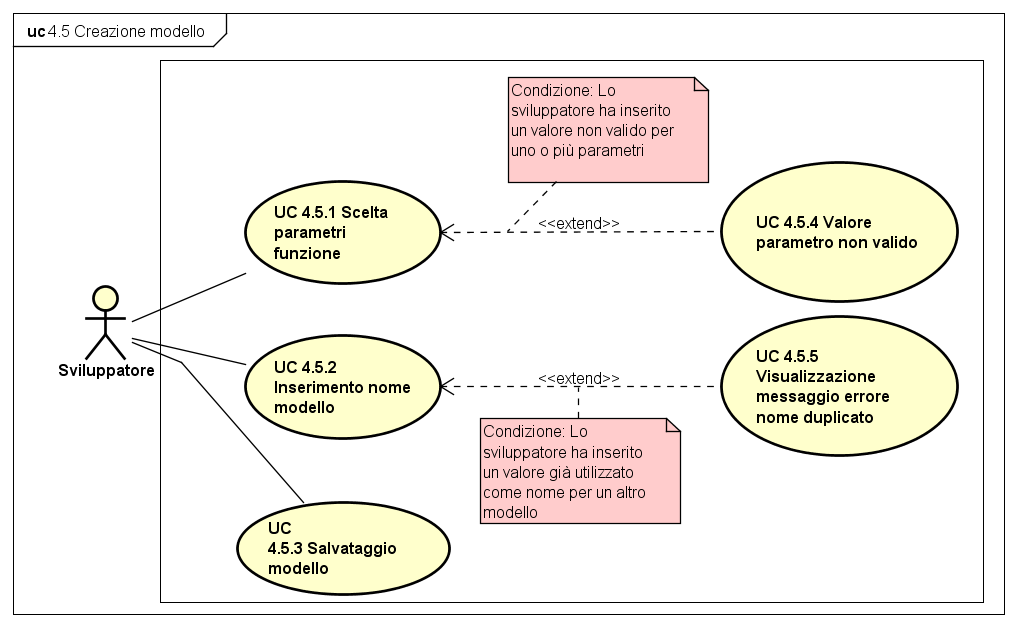
\includegraphics[width=10cm, keepaspectratio]{img/UC450.png} 
	\caption{Caso d'uso UC 4.5}\label{fig:450}
\end{figure}
\begin{itemize}
	\item[•]\textbf{Attori}: Sviluppatore;
	\item[•]\textbf{Descrizione}: lo sviluppatore esegue il download dei dati d'interesse;
	\item[•]\textbf{Precondizione}: lo sviluppatore visualizza i dati in ordine cronologico, e nel caso siano applicati filtri, vede solo i dati che rispettano tali filtri;
	\item[•]\textbf{Postcondizione}: lo sviluppatore scarica un file contenente le analisi grammaticali in formato anonimo;
	\item[•]\textbf{Flusso degli eventi}:
	\begin{enumerate}
		\item UC 4.5.1 - Scelta contenuti download;
		\item UC 4.5.2 - Scelta formato file;
		\item UC 4.5.3 - Scelta formato archivio.
	\end{enumerate}
\end{itemize}

\subsubsection{UC 4.5.1 - Scelta contenuti download}
\begin{itemize}
	\item[•]\textbf{Attori}: Sviluppatore;
	\item[•]\textbf{Descrizione}: lo sviluppatore sceglie gli elementi di interesse che vuole siano scaricati una volta completata la procedura di download;
	\item[•]\textbf{Precondizione}: lo sviluppatore visualizza le preposizioni in base ai filtri stabiliti;
	\item[•]\textbf{Postcondizione}: lo sviluppatore visualizza i contenuti che intende scaricare, come ad esempio lo storico di una frase;
	\item[•]\textbf{Flusso degli eventi}: lo sviluppatore seleziona dall'elenco, eventualmente filtrato, le proposizioni d'interesse, come ad esempio quelle provenienti da i soli docenti selezionati.
\end{itemize}

\subsubsection{UC 4.5.2 - Scelta formato file}
\begin{itemize}
	\item[•]\textbf{Attori}: Sviluppatore;
	\item[•]\textbf{Descrizione}:  lo sviluppatore seleziona da un elenco prestabilito il formato dei file che intende scaricare;
	\item[•]\textbf{Precondizione}: lo sviluppatore non ha stabilito il formato dei file che intende scaricare;
	\item[•]\textbf{Postcondizione}: lo sviluppatore ha stabilito il formato dei file che intende scaricare;
	\item[•]\textbf{Flusso degli eventi principale}:  lo sviluppatore seleziona dall'elenco prestabilito un'opzione che determina il formato dei file che contengono i dati precedentemente scelti.
\end{itemize}

\subsubsection{UC 4.5.3 - Scelta formato archivio}
\begin{itemize}
	\item[•]\textbf{Attori}: Sviluppatore;
	\item[•]\textbf{Descrizione}: lo sviluppatore seleziona da un elenco prestabilito il formato dell'archivio compresso con cui vuole che i dati d'interesse siano compressi;
	\item[•]\textbf{Precondizione}: il formato dell'archivio contenente i dati d'interesse non è definito;
	\item[•]\textbf{Postcondizione}: il formato dell'archivio contenente i dati d'interesse è stato definito;
	\item[•]\textbf{Flusso degli eventi}: lo sviluppatore seleziona dall'elenco prestabilito un'opzione che determina il formato dell'archivio che contiene i file relativi ai dati precedentemente scelti.
\end{itemize}


\subsubsection{UC 4.6 - Creazione modello}
\begin{figure}[H]
	\centering
	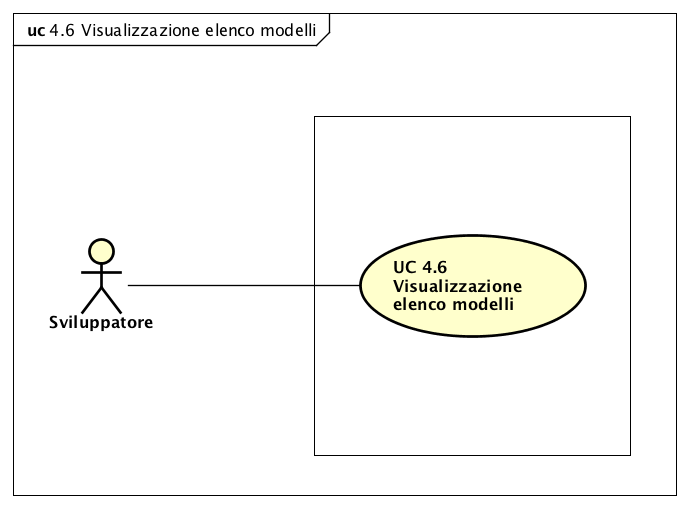
\includegraphics[width=17cm, keepaspectratio]{img/UC460.png} 
	\caption{Caso d'uso UC 4.6}\label{fig:460}
\end{figure}
\begin{itemize}
	\item[•]\textbf{Attori}: Sviluppatore;
	\item[•]\textbf{Descrizione}: lo sviluppatore crea un nuovo modello;
	\item[•]\textbf{Precondizione}: lo sviluppatore non ha creato il modello;
	\item[•]\textbf{Postcondizione}: lo sviluppatore ha creato un nuovo modello;
	\item[•]\textbf{Flusso degli eventi}:  
	\begin{enumerate}
		\item UC 4.6.1 - Scelta parametri funzione;
		\item UC 4.6.2 - Inserimento nome modello;
		\item UC 4.6.3 - Salvataggio modello.
	\end{enumerate}
	\item[•]\textbf{Estensioni}:  
	\begin{enumerate}
		\item UC 4.6.4 - Valore parametro non valido;
		\item UC 4.6.5 - Visualizzazione messaggio errore nome duplicato.
	\end{enumerate}
\end{itemize}

\subsubsection{UC 4.6.1 - Scelta parametri funzione}
\begin{itemize}
	\item[•]\textbf{Attori}: Sviluppatore;
	\item[•]\textbf{Descrizione}: lo sviluppatore sceglie i parametri della funzione per la creazione di un nuovo modello con i relativi valori associati;
	\item[•]\textbf{Precondizione}: lo sviluppatore non ha scelto i parametri da inserire;
	\item[•]\textbf{Postcondizione}: lo sviluppatore ha inserito i parametri per la creazione di un nuovo modello;
	\item[•]\textbf{Flusso degli eventi}:  lo sviluppatore inserisce tutti i parametri necessari che verranno impiegati nella realizzazione del modello;
	\item[•] \textbf{Estensioni}: 
	\begin{enumerate}
		\item UC 4.6.4 - Valore parametro non valido.
	\end{enumerate}
\end{itemize}

\subsubsection{UC 4.6.2 - Inserimento nome modello}
\begin{itemize}
	\item[•]\textbf{Attori}: Sviluppatore;
	\item[•]\textbf{Descrizione}: lo sviluppatore inserisce il nome per il modello che intende salvare;
	\item[•]\textbf{Precondizione}: lo sviluppatore non ha inserito il nome del modello;
	\item[•]\textbf{Postcondizione}: lo sviluppatore ha inserito il nome del modello;
	\item[•]\textbf{Flusso degli eventi}: lo sviluppatore inserisce una stringa che definisce il nome del modello che verrà memorizzato;
	\item[•] \textbf{Estensioni}: 
	\begin{enumerate}
		\item UC 4.5.5 - Visualizzazione messaggio errore nome duplicato.
	\end{enumerate}
\end{itemize}

\subsubsection{UC 4.6.3 - Salvataggio modello}
\begin{itemize}
	\item[•]\textbf{Attori}: Sviluppatore;
	\item[•]\textbf{Descrizione}: lo sviluppatore salva il modello di cui ha definito il nome;
	\item[•]\textbf{Precondizione}: lo sviluppatore ha inserito il nome del modello;
	\item[•]\textbf{Postcondizione}: lo sviluppatore ha salvato il modello;
	\item[•]\textbf{Flusso degli eventi}: lo sviluppatore seleziona l'opzione relativa al salvataggio che comporta il salvataggio del modello.
\end{itemize}

\subsubsection{UC 4.6.4 - Valore parametro non valido}
\begin{itemize}
	\item[•]\textbf{Attori}: Sviluppatore;
	\item[•]\textbf{Descrizione}: il sistema segnala un messaggio di errore relativo al valore del parametro non valido;
	\item[•]\textbf{Precondizione}: lo sviluppatore ha inserito il valore del parametro;
	\item[•]\textbf{Postcondizione}: lo sviluppatore visualizza un messaggio di errore relativo al valore del parametro non valido;
	\item[•]\textbf{Flusso degli eventi}:  lo sviluppatore ha inserito un valore per il parametro non valido pertanto visualizza un messaggio d'errore.
\end{itemize}
\subsubsection{UC 4.6.5 - Visualizzazione messaggio errore nome duplicato}
\begin{itemize}
	\item[•]\textbf{Attori}: Sviluppatore;
	\item[•]\textbf{Descrizione}: lo sviluppatore visualizza un messaggio di errore relativo all'inserimento di un modello avente lo stesso nome di uno già inserito;
	\item[•]\textbf{Precondizione}: lo sviluppatore ha inserito il nome del modello;
	\item[•]\textbf{Postcondizione}: lo sviluppatore visualizza il messaggio di errore e inserisce un nuovo nome;
	\item[•]\textbf{Flusso degli eventi}:  lo sviluppatore visualizza il messaggio di errore e può inserire una stringa che definisce il nome del modello che verrà memorizzato.
\end{itemize}

\subsubsection{UC 4.6.6 - Interruzione inserimento modello}
\begin{itemize}
	\item[•]\textbf{Attori}: Sviluppatore;
	\item[•]\textbf{Descrizione}: lo sviluppatore interrompe l'inserimento del modello;
	\item[•]\textbf{Precondizione}: lo sviluppatore sta inserendo il modello;
	\item[•]\textbf{Postcondizione}: nessun nuovo modello è stato inserito;
	\item[•]\textbf{Flusso degli eventi}: lo sviluppatore interrompe l'inserimento del modello abbandonando la pagina.
\end{itemize}
\subsubsection{UC 4.7 - Visualizzazione elenco modelli}
\begin{itemize}
	\item[•]\textbf{Attori}: Sviluppatore;
	\item[•]\textbf{Descrizione}: lo sviluppatore visualizza l'elenco dei propri modelli realizzati;
	\item[•]\textbf{Precondizione}: lo sviluppatore si è autenticato nel sistema;
	\item[•]\textbf{Postcondizione}: lo sviluppatore visualizza l'elenco dei propri modelli;
	\item[•]\textbf{Flusso degli eventi}:  lo sviluppatore seleziona la voce del menù relativa ai modelli e ne visualizza l'elenco.
\end{itemize}


\subsubsection{UC 4.8 - Visualizzazione contenuto modello} 
\begin{itemize}
	\item[•]\textbf{Attori}: Sviluppatore;
	\item[•]\textbf{Descrizione}: lo sviluppatore visualizza il contenuto del modello selezionato;
	\item[•]\textbf{Precondizione}: lo sviluppatore visualizza l'elenco dei modelli (UC 4.6);
	\item[•]\textbf{Postcondizione}: lo sviluppatore visiona il contenuto del modello selezionato;
	\item[•]\textbf{Flusso degli eventi}: lo sviluppatore seleziona dall'elenco dei modelli quello d'interesse e ne visualizza il contenuto.
\end{itemize}

\subsubsection{UC 4.9 - Scaricamento modello}
\begin{itemize}
	\item[•]\textbf{Attori}: Sviluppatore;
	\item[•]\textbf{Descrizione}: lo sviluppatore ottiene un file contenente il modello precedentemente creato;
	\item[•]\textbf{Precondizione}: lo sviluppatore visualizza il contenuto del modello che intende scaricare;
	\item[•]\textbf{Postcondizione}: lo sviluppatore ottiene un file contenente il modello selezionato;
	\item[•]\textbf{Flusso degli eventi}: lo sviluppatore seleziona l'opzione di scaricamento e ottiene un file contenente il modello.
\end{itemize}

\subsubsection{UC 4.10 - Eliminazione modello}
\begin{itemize}
	\item[•]\textbf{Attori}: Sviluppatore;
	\item[•]\textbf{Descrizione}: lo sviluppatore elimina il modello;
	\item[•]\textbf{Precondizione}: lo sviluppatore visualizza l'elenco dei propri modelli;
	\item[•]\textbf{Postcondizione}: lo sviluppatore ha eliminato il modello; 
	\item[•]\textbf{Flusso degli eventi}: 
	\begin{enumerate}
		\item Selezione modello;
		\item Selezione procedura eliminazione.
	\end{enumerate}   
\end{itemize}


\subsubsection{UC 4.11 - Modifica dati utente}
\begin{figure}[H]
	\centering
	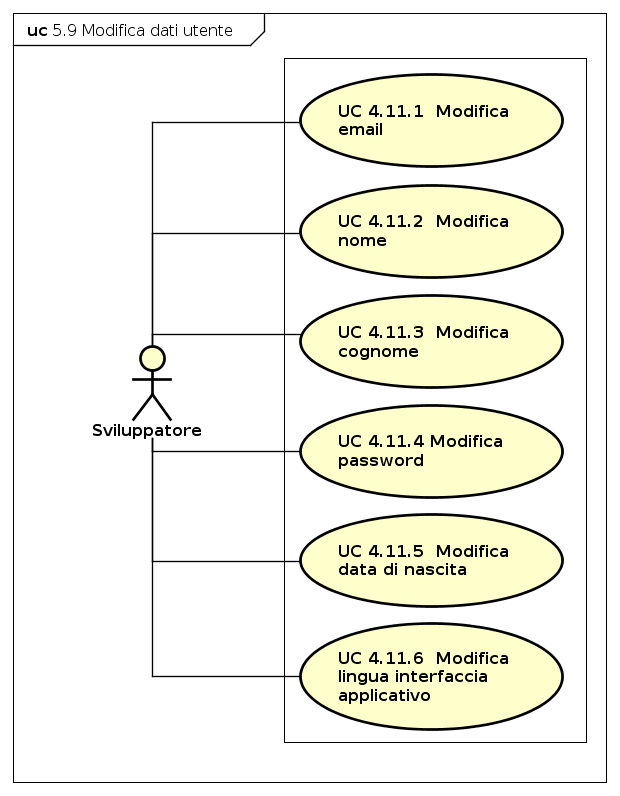
\includegraphics[width=12cm, keepaspectratio]{img/UC411.png} 
	\caption{Caso d'uso UC 4.11:  Modifica dati utente per Sviluppatore}\label{fig:411}
\end{figure}
\begin{itemize}
	\item[•]\textbf{Attori}: Sviluppatore;
	\item[•]\textbf{Descrizione}: lo sviluppatore modifica i propri dati personali, cioè tutti i dati personali inseriti in fase di registrazione;
	\item[•]\textbf{Precondizione}: lo sviluppatore visualizza la propria dashboard;
	\item[•]\textbf{Postcondizione}: lo sviluppatore ha modificato uno o più dati personali; 
	\item[•]\textbf{Flusso degli eventi}: 
	\begin{enumerate}
		\item Selezione procedura modifica dati personali;
		\item UC 4.11.1 - Modifica email; 
		\item UC 4.11.2 - Modifica nome;
		\item UC 4.11.3 - Modifica cognome;
		\item UC 4.11.4 - Modifica password;
		\item UC 4.11.5 - Modifica data di nascita;
		\item UC 4.11.6 - Modifica lingua interfaccia applicativo;
		\item Conferma modifica dati.
	\end{enumerate}
	\item[•] \textbf{Estensioni}:	
	\begin{enumerate}
		\item UC 4.11.7 - Interruzione modifica dati utente.
	\end{enumerate}
\end{itemize}
\subsubsection{UC 4.11.1 - Modifica email}
\begin{itemize}
	\item[•]\textbf{Attori}: Sviluppatore;
	\item[•]\textbf{Descrizione}: lo sviluppatore modifica la propria email;
	\item[•]\textbf{Precondizione}: lo sviluppatore sta modificando i propri dati personali;
	\item[•]\textbf{Postcondizione}: lo sviluppatore ha modificato la propria email; 
	\item[•]\textbf{Flusso degli eventi}: 
	\begin{enumerate}
		\item Selezione campo email;
		\item Modifica la stringa che rappresenta la propria email.
	\end{enumerate}
	\item[•]\textbf{Estensioni}: 
	\begin{enumerate}
		\item UC 4.11.7 - Interruzione modifica dati utente.
	\end{enumerate}
\end{itemize}
\subsubsection{UC 4.11.2 - Modifica nome}
\begin{itemize}
	\item[•]\textbf{Attori}: Sviluppatore;
	\item[•]\textbf{Descrizione}: lo sviluppatore modifica il proprio nome;
	\item[•]\textbf{Precondizione}: lo sviluppatore sta modificando i propri dati personali;
	\item[•]\textbf{Postcondizione}: lo sviluppatore ha modificato il proprio nome; 
	\item[•]\textbf{Flusso degli eventi}: 
	\begin{enumerate}
		\item Selezione campo nome;
		\item Modifica la stringa che rappresenta il nome.
	\end{enumerate}
	\item[•]\textbf{Estensioni}: 
	\begin{enumerate}
		\item UC 4.11.7 - Interruzione modifica dati utente.
	\end{enumerate}
\end{itemize}
\subsubsection{UC 4.11.3 - Modifica cognome}
\begin{itemize}
	\item[•]\textbf{Attori}: Sviluppatore;
	\item[•]\textbf{Descrizione}: lo sviluppatore modifica il proprio cognome;
	\item[•]\textbf{Precondizione}: lo sviluppatore sta modificando i propri dati personali;
	\item[•]\textbf{Postcondizione}: lo sviluppatore ha modificato il proprio cognome; 
	\item[•]\textbf{Flusso degli eventi}: 
	\begin{enumerate}
		\item Selezione campo cognome;
		\item Modifica la stringa che rappresenta il cognome.
	\end{enumerate}
	\item[•]\textbf{Estensioni}: 
	\begin{enumerate}
		\item UC 4.11.7 - Interruzione modifica dati utente.
	\end{enumerate}
\end{itemize}
\subsubsection{UC 4.11.4 - Modifica password}
\begin{figure}[H]
	\centering
	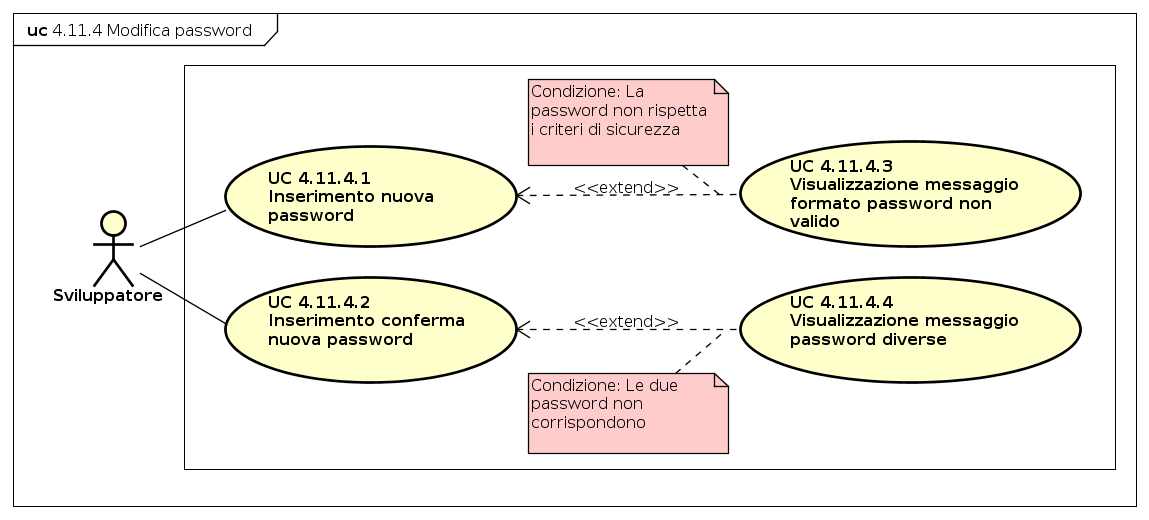
\includegraphics[width=15cm, keepaspectratio]{img/UC4114.png} 
	\caption{Caso d'uso UC 4.11.4, modifica password per Sviluppatore}\label{fig:4114}
\end{figure}
\begin{itemize}
	\item[•]\textbf{Attori}: Sviluppatore;
	\item[•]\textbf{Descrizione}: lo sviluppatore modifica il proprio cognome;
	\item[•]\textbf{Precondizione}: lo sviluppatore sta modificando i propri dati personali;
	\item[•]\textbf{Postcondizione}: lo sviluppatore ha modificato il proprio cognome; 
	\item[•]\textbf{Flusso degli eventi}: 
	\begin{enumerate}
		\item UC 4.11.4.1 - Inserimento nuova password;
		\item UC 4.11.4.2 - Inserimento conferma nuova password.
	\end{enumerate}
	\item[•]\textbf{Estensioni}: 
	\begin{enumerate}
		\item UC 4.11.7 - Interruzione modifica dati utente.
	\end{enumerate}
\end{itemize}

\subsubsection{UC 4.11.4.1 - Inserimento nuova password}
\begin{itemize}
	\item[•]\textbf{Attori}: Sviluppatore;
	\item[•]\textbf{Descrizione}: lo sviluppatore inserisce la nuova password;
	\item[•]\textbf{Precondizione}: lo sviluppatore sta modificando i propri dati personali;
	\item[•]\textbf{Postcondizione}: lo sviluppatore ha inserito il valore della nuova password; 
	\item[•]\textbf{Flusso degli eventi}: 
	\begin{enumerate}
		\item Selezione campo dati relativo alla nuova password;
		\item Inserimento stringa rappresentante la password.
	\end{enumerate}
	\item[•]\textbf{Estensioni}:
	\begin{enumerate}
		\item UC 4.11.4.3 - Visualizzazione messaggio formato password non valido;
		\item UC 4.11.7 - Interruzione modifica dati utente.
	\end{enumerate}
\end{itemize}

\subsubsection{UC 4.11.4.2 - Inserimento conferma nuova password}
\begin{itemize}
	\item[•]\textbf{Attori}: Sviluppatore;
	\item[•]\textbf{Descrizione}: lo sviluppatore inserisce conferma la nuova password, reinserendola nell'apposito campo;
	\item[•]\textbf{Precondizione}: lo sviluppatore sta modificando i propri dati personali;
	\item[•]\textbf{Postcondizione}: lo sviluppatore ha inserito il valore del campo conferma nuova password; 
	\item[•]\textbf{Flusso degli eventi}: 
	\begin{enumerate}
		\item Selezione campo dati relativo alla conferma nuova password;
		\item Inserimento stringa rappresentante la password;
	\end{enumerate}
	\item[•]\textbf{Estensioni}:
	\begin{enumerate}
		\item UC 4.11.4.4 - Visualizzazione messaggio password diverse;
		\item UC 4.11.7 - Interruzione modifica dati utente.
	\end{enumerate}
\end{itemize}

\subsubsection{UC 4.11.4.3 - Visualizzazione messaggio formato password non valido}
\begin{itemize}
	\item[•]\textbf{Attori}: Sviluppatore;
	\item[•]\textbf{Descrizione}: lo sviluppatore ha inserito una password con un formato non valido;
	\item[•]\textbf{Precondizione}: lo sviluppatore sta modificando i propri dati personali;
	\item[•]\textbf{Postcondizione}: lo sviluppatore visualizza un messaggio di errore relativo all'inserimento di una password che non rispetta un formato valido; 
	\item[•]\textbf{Flusso degli eventi}: lo sviluppatore ha inserito una password che non rispetta i criteri accettati dal sistema, pertanto riceve un messaggio che indica la presenza di un formato non adatto;
	\item[•]\textbf{Estensioni}: 
	\begin{enumerate}
		\item UC 4.11.7 - Interruzione modifica dati utente.
	\end{enumerate}
\end{itemize}

\subsubsection{UC 4.11.4.4 - Visualizzazione messaggio password diverse}
\begin{itemize}
	\item[•]\textbf{Attori}: Sviluppatore;
	\item[•]\textbf{Descrizione}: lo sviluppatore ha inserito un valore di conferma password che non corrisponde al valore della nuova password inserita precedentemente, pertanto visualizza un messaggio che indica che le due password non corrispondono;
	\item[•]\textbf{Precondizione}: lo sviluppatore ha inserito il valore del campo conferma nuova password;
	\item[•]\textbf{Postcondizione}: lo sviluppatore visualizza un messaggio di errore relativo all'inserimento di una password che non combacia con quella inserita nel campo nuova password; 
	\item[•]\textbf{Flusso degli eventi}: lo sviluppatore ha inserito una password che non combacia con quella inserita nel campo nuova password, pertanto riceve un messaggio che indica la presenza di tale difformità;
	\item[•]\textbf{Estensioni}: 
	\begin{enumerate}
		\item UC 4.11.7 - Interruzione modifica dati utente.
	\end{enumerate}
\end{itemize}

\subsubsection{UC 4.11.5 - Modifica data di nascita}
\begin{itemize}
	\item[•]\textbf{Attori}: Sviluppatore;
	\item[•]\textbf{Descrizione}: lo sviluppatore modifica il proprio cognome;
	\item[•]\textbf{Precondizione}: lo sviluppatore sta modificando i propri dati personali;
	\item[•]\textbf{Postcondizione}: lo sviluppatore ha modificato il proprio cognome; 
	\item[•]\textbf{Flusso degli eventi}: 
	\begin{enumerate}
		\item Selezione campo data di nascita;
		\item Modifica la stringa che rappresenta la data di nascita, inserendo il valore corretto.
	\end{enumerate}
	\item[•]\textbf{Estensioni}: 
	\begin{enumerate}
		\item UC 4.11.7 - Interruzione modifica dati utente.
	\end{enumerate}
\end{itemize}
\subsubsection{UC 4.11.6 - Modifica lingua interfaccia applicativo}
\begin{itemize}
	\item[•]\textbf{Attori}: Sviluppatore;
	\item[•]\textbf{Descrizione}: lo sviluppatore modifica la lingua dell'applicativo;
	\item[•]\textbf{Precondizione}: lo sviluppatore sta modificando i propri dati personali;
	\item[•]\textbf{Postcondizione}: lo sviluppatore ha modificato la lingua dell'applicativo; 
	\item[•]\textbf{Flusso degli eventi}: 
	\begin{enumerate}
		\item Selezione campo dati lingua applicativo;
		\item Selezione da un elenco predefinito la lingua dell'applicativo desiderata.
	\end{enumerate}
	\item[•]\textbf{Estensioni}: 
	\begin{enumerate}
		\item UC 4.11.7 - Interruzione modifica dati utente.
	\end{enumerate}
\end{itemize}

\subsubsection{UC 4.11.7 - Interruzione modifica dati utente}
\begin{itemize}
	\item[•]\textbf{Attori}: Sviluppatore;
	\item[•]\textbf{Descrizione}: lo sviluppatore interrompe la procedura di modifica dei dati utente;
	\item[•]\textbf{Precondizione}: lo sviluppatore sta modificando i propri dati;
	\item[•]\textbf{Postcondizione}: lo sviluppatore abbandona la procedura e nessuna modifica è stata effettuata nel sistema; 
	\item[•]\textbf{Flusso degli eventi}: lo sviluppatore abbandona la pagina di modifica dei dati e viene reindirizzato alla dashboard.
\end{itemize}

\subsubsection{UC 4.12 - Logout}
\begin{itemize}
	\item[•]\textbf{Attori}: Sviluppatore;
	\item[•]\textbf{Descrizione}: lo sviluppatore effettua il logout dal sistema e viene reindirizzato alla pagina di login;
	\item[•]\textbf{Precondizione}: lo sviluppatore si è autenticato;
	\item[•]\textbf{Postcondizione}: lo sviluppatore ha chiuso la sessione e viene reindirizzato alla pagina di autenticazione; 
	\item[•]\textbf{Flusso degli eventi}: lo sviluppatore seleziona il collegamento al logout e termina la sessione.
\end{itemize}


\subsubsection{UC 4.13 - Visualizzazione dati filtrati}
\begin{itemize}
	\item[•]\textbf{Attori}: Sviluppatore;
	\item[•]\textbf{Descrizione}: selezionato uno o più filtri, i dati vengono mostrati secondo i vincoli inseriti;
	\item[•]\textbf{Precondizione}: i valori di uno o più filtri sono stati inseriti;
	\item[•]\textbf{Postcondizione}: lo sviluppatore visualizza solamente le preposizioni che rispettano i filtri inseriti;
	\item[•]\textbf{Flusso degli eventi}: lo sviluppatore inserisce un filtro e visualizza le preposizioni, la data d'inserimento, l'autore e le correzioni inserite che rispettano tale filtro.
\end{itemize}

\subsubsection{UC 4.14 - Rimozione filtro periodo temporale}
\begin{itemize}
	\item[•]\textbf{Attori}: Sviluppatore;
	\item[•]\textbf{Descrizione}: lo sviluppatore cancella il valore del filtro periodo temporale che indica un arco di tempo in cui le preposizioni sono state inserite;
	\item[•]\textbf{Precondizione}: il filtro periodo temporale è impostato e lo sviluppatore visualizza solamente le preposizioni inserite in quel periodo temporale;
	\item[•]\textbf{Postcondizione}: il filtro periodo temporale è stato rimosso e le preposizioni visualizzate non rispettano più quel filtro;
	\item[•]\textbf{Flusso degli eventi}: lo sviluppatore seleziona il filtro periodo temporale e lo rimuove.
\end{itemize}

\subsubsection{UC 4.15 - Rimozione filtro fonte}
\begin{itemize}
	\item[•]\textbf{Attori}: Sviluppatore;
	\item[•]\textbf{Descrizione}: lo sviluppatore cancella il valore del filtro fonte, cioè le frasi provenienti da uno o più autori;
	\item[•]\textbf{Precondizione}: il filtro fonte è impostato e lo sviluppatore visualizza solamente le preposizioni inserite da una o più fonti;
	\item[•]\textbf{Postcondizione}: il filtro periodo fonte è stato rimosso e le preposizioni visualizzate non rispettano più quel filtro;
	\item[•]\textbf{Flusso degli eventi}: lo sviluppatore seleziona il filtro fonte e lo rimuove.
\end{itemize}

\subsubsection{UC 4.16 - Rimozione filtro lingue}
\begin{itemize}
	\item[•]\textbf{Attori}: Sviluppatore;
	\item[•]\textbf{Descrizione}: lo sviluppatore cancella il valore del filtro lingue che indica le preposizioni inserite in tali lingue;
	\item[•]\textbf{Precondizione}: il filtro lingue è impostato e lo sviluppatore visualizza solamente le preposizioni inserite scritte in tali lingue;
	\item[•]\textbf{Postcondizione}: il filtro lingue è stato rimosso e le preposizioni vengono mostrate indipendentemente dalla lingua di inserimento;
	\item[•]\textbf{Flusso degli eventi}: lo sviluppatore seleziona il filtro lingue e lo rimuove.
\end{itemize}

\subsubsection{UC 4.17 - Rimozione filtro attendibilità}
\begin{itemize}
	\item[•]\textbf{Attori}: Sviluppatore;
	\item[•]\textbf{Descrizione}: lo sviluppatore cancella il valore del filtro attendibilità, cioè le frasi provenienti da fonti avente una determinata attendibilità espressa in formato numerico;
	\item[•]\textbf{Precondizione}: il filtro attendibilità è impostato e lo sviluppatore visualizza solamente le preposizioni inserite da fonti con quel determinato valore di affidabilità;
	\item[•]\textbf{Postcondizione}: il filtro attendibilità è stato rimosso e le preposizioni visualizzate non rispettano più quel filtro;
	\item[•]\textbf{Flusso degli eventi}: lo sviluppatore seleziona il filtro attendibilità e rimuove il suo valore.
\end{itemize}
\newpage
\subsection{Amministratore}

\subsubsection{Panoramica amministratore}
\begin{figure}[H]
\centering
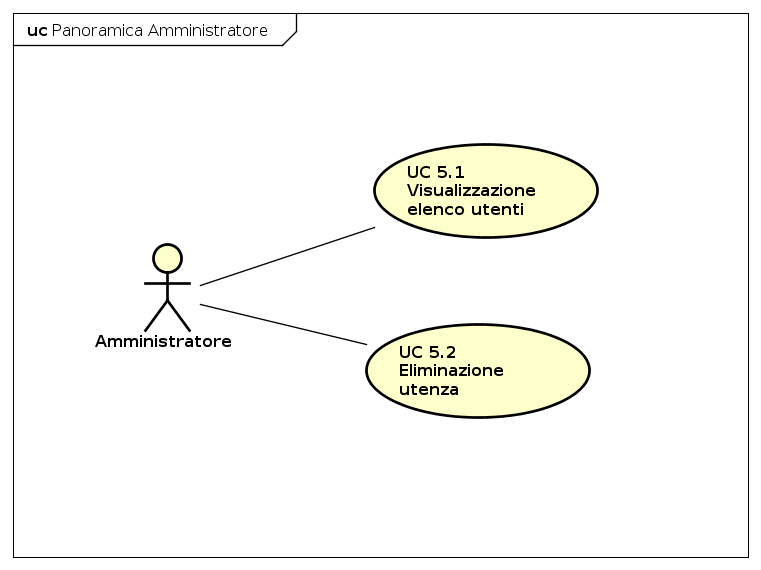
\includegraphics[width=17cm, height= 20cm]{img/PanoramicaAmministratore.png} 
\caption{Panoramica amministratore}
\end{figure}


\subsubsection{UC 5.1 - Visualizzazione dashboard}

\begin{itemize}
\item \textbf{Attore}: Amministratore; 
\item \textbf{Descrizione}: l'amministratore visualizza la propria dashboard;
\item \textbf{Precondizione}: l'amministratore si è autenticato;
\item \textbf{Postcondizione}: l'amministratore è visualizza la sua dashboard;
\item \textbf{Flusso degli eventi}: l'amministratore accede alla propria dashboard personale e può effettuare modifiche al sistema;
\end{itemize}

\subsubsection{UC 5.2 - Visualizzazione utenti registrati}

\begin{itemize}
\item \textbf{Attore}: Amministratore;
\item \textbf{Descrizione}: l'amministratore visualizza l'elenco degli utenti registrati nel sistema;
\item \textbf{Precondizione}: l'amministratore si è autenticato;
\item \textbf{Postcondizione}: l'amministratore visualizza tutti gli utenti registrati nel sistema;
\item \textbf{Flusso degli eventi}: l'amministratore accede alla propria dashboard e visualizza l'elenco degli utenti registrati nel sistema.
\end{itemize}

\subsubsection{UC 5.3 - Filtraggio utenti}
\begin{itemize}
\item \textbf{Attore}: Amministratore;
\item \textbf{Descrizione}: l'amministratore può filtrare gli utenti;
\item \textbf{Precondizione}: l'amministratore si è autenticato;
\item \textbf{Postcondizione}: l'amministratore visualizza la lista degli utenti in base ai filtri applicati;
\item \textbf{Flusso degli eventi}: l'amministratore visualizza elenco utenti ed ha la possibilità di filtrate.
\end{itemize}
\subsubsection{UC 5.4 - Visualizzazione dettaglio utente}
\begin{itemize}
\item \textbf{Attore}: Amministratore;
\item \textbf{Descrizione}: l'amministratore visualizza in dettaglio un utente specifico;
\item \textbf{Precondizione}: l'amministratore visualizza la lista degli utenti;
\item \textbf{Postcondizione}: l'amministratore visualizza le informazioni personali dell'utente;
\item \textbf{Flusso degli eventi}: l'amministratore visualizza l'elenco utenti ed ha la possibilità di visualizzare un utente nel dettaglio.
\end{itemize}


\subsubsection{UC 5.5 - Eliminazione utenza}
\begin{itemize}
\item \textbf{Attore}: Amministratore;
\item \textbf{Descrizione}: l'amministratore elimina un'utenza dal sistema;
\item \textbf{Precondizione}: l'amministratore visualizza l'elenco degli utenti registrati nel sistema;
\item \textbf{Postcondizione}: l'amministratore ha eliminato l'utenza dal sistema;
\item \textbf{Flusso degli eventi}: l'amministratore visualizza elenco utenti ed ha la possibilità di eliminare un'utenza.
\end{itemize}


\subsubsection{UC 5.6 - Visualizzazione richieste sviluppatori}
\begin{itemize}
\item \textbf{Attore}: Amministratore;
\item \textbf{Descrizione}: l'amministratore visualizza le richieste degli utenti;
\item \textbf{Precondizione}: l'amministratore si trova nella dashboard;
\item \textbf{Postcondizione}: l'amministratore visualizza l'elenco delle richieste in sospeso;
\item \textbf{Flusso degli eventi}:  l'amministratore visualizza tutte le richieste degli utenti che vogliono ottenere il ruolo di sviluppatore nel sistema.
\end{itemize}

\subsubsection{UC 5.7 - Attivazione utenza sviluppatore}
\begin{itemize}
\item \textbf{Attore}: Amministratore;
\item \textbf{Descrizione}: l'amministratore può attivare utenza in sospeso;
\item \textbf{Precondizione}: l'amministratore visualizza la lista delle richieste in sospeso degli sviluppatori;
\item \textbf{Postcondizione}: l'utenza dello sviluppatore è stata attivata e lo sviluppatore può quindi accedere al sistema;
\item \textbf{Flusso degli eventi}: l'amministratore attiva un utente che ha fatto richiesta come sviluppatore;
\end{itemize}

\subsubsection{UC 5.8 - Rifiuto richiesta sviluppatore}
\begin{itemize}
\item \textbf{Attore}: Amministratore;
\item \textbf{Descrizione}: l'amministratore può rifiutare utenza in sospeso;
\item \textbf{Precondizione}: l'amministratore visualizza la lista delle richieste in sospeso degli sviluppatori;
\item \textbf{Postcondizione}: l'utenza dello sviluppatore è stata rifiutata;
\item \textbf{Flusso degli eventi}: l'amministratore rifiuta la richiesta avanzata da uno sviluppatore.
\end{itemize}




\section{Requisiti}

\subsection{Classificazione dei requisiti}\mbox{}\\
I vari requisiti potranno provenire dalle seguenti fonti:
\begin{itemize}
	\item[•] \textbf{Capitolato}: il requisito è stato scritto esplicitamente nel documento fornito dalla proponente;
	\item[•] \textbf{Verbali interni e studio di fattibilità}: il requisito è emerso durante la discussione del capitolato tra gli analisti;
	\item[•] \textbf{Casi d'uso}: il requisito è il risultato dell'analisi di uno o più casi d'uso.
\end{itemize}

I vari requisiti devono essere classificati secondo la seguente convenzione:
\begin{center}
	R-[Importanza][Tipo][Identificativo]
\end{center}
Dove:
\begin{itemize}
	\item[•] Importanza, indica se il requisito è:
	\begin{itemize}
		\item[1]: Requisito obbligatorio;
		\item[2]: Requisito desiderabile;
		\item[3]: Requisito opzionale.
	\end{itemize}
	\item[•] Tipo, indica se il requisito è:
	\begin{itemize}
		\item[F]: Requisito funzionale;
		\item[Q]: Requisito di qualità;
		\item[P]: Requisito prestazionale;
		\item[V]: Requisito di vincolo.
	\end{itemize}
	\item[•] Identificativo: ovvero un codice univoco che contraddistingue il requisito.
\end{itemize}

\subsection{Requisiti funzionali} 
\renewcommand{\arraystretch}{1.5}
\def\tabularxcolumn#1{m{#1}}
\begin{tabularx}{\textwidth}{cXccc}
 
\rowcolor{greySWEight}
   \textcolor{white}{\textbf{Identificativo}} &
   \textcolor{white}{\textbf{Descrizione}}&
   \textcolor{white}{\textbf{Importanza}}&
   \textcolor{white}{\textbf{Tipo}}&
   \textcolor{white}{\textbf{Fonte}}\endhead

		R-1F001 & Un utente non autenticato può autenticarsi nel sistema & Obbligatorio & Funzionale & Capitolato \\
		R-2F001 & Un utente può selezionare la lingua dell'interfaccia desiderata & Desiderabile & Funzionale & Capitolato \\
		R-1F002 & Un utente non autenticato deve inserire la propria email per autenticarsi & Obbligatorio & Funzionale & Interno \\
		R-1F003 & Un utente non autenticato deve inserire la propria password per autenticarsi & Obbligatorio & Funzionale & Interno \\
		R-1F004 & Un utente non autenticato può registrarsi & Obbligatorio & Funzionale & Interno \\
		R-1F005 & Un utente non autenticato deve inserire l'email per registrarsi & Obbligatorio & Funzionale & Interno \\
		R-1F006 & Un utente non autenticato deve inserire il proprio nome per registrarsi & Obbligatorio & Funzionale & Interno \\
		R-1F007 & Un utente non autenticato deve inserire il proprio cognome per registrarsi & Obbligatorio & Funzionale & Interno \\
		R-1F008 & Un utente non autenticato deve inserire la password per registrarsi & Obbligatorio & Funzionale & Interno \\
		R-1F009 & Un utente non autenticato deve re-inserire la password per registrarsi & Obbligatorio & Funzionale & Interno \\
		R-2F002 & Un utente può inserire la propria data di nascita & Desiderabile & Funzionale & Interno \\
		R-1F010 & Un utente non autenticato deve selezionare il ruolo desiderato in fase di registrazione & Obbligatorio & Funzionale & Interno \\
		R-1F011 & Un utente non autenticato può recuperare le proprie credenziali & Obbligatorio & Funzionale & Interno \\
		R-1F012 & Un insegnante può visualizzare la propria dashboard & Obbligatorio & Funzionale & Capitolato \\
		R-1F013 & Un insegnante può inserire un nuovo esericizio di analisi grammaticale & Obbligatorio & Funzionale & Capitolato \\
		R-3F001 & Un insegnante può selezionare la lingua dell'esercizio & Opzionale & Funzionale & Capitolato \\
		R-1F014 & Un insegnate deve inserire il testo dell'esercizio & Obbligatorio & Funzionale & Interno \\
		R-1F015 & Un insegnante può usufruire del servizio di correzione automatica da parte della libreria di Pos-Tagging & Obbligatorio & Funzionale & Capitolato \\
		R-1F016 & Un insegnante può modificare il tag automatico di una parola & Obbligatorio & Funzionale & Interno \\
		R-2F003 & Un insegnante può inserire un tag per la soluzione alternativa & Desiderabile & Funzionale & Capitolato \\
		R-3F002 & Un insegnante può assegnare uno o più esercizi & Opzionale & Funzionale & Capitolato \\
		R-1F017 & Un insegnante può assegnare uno o più esercizi a determinate classi e/o alunni & Obbligatorio & Funzionale & Capitolato \\
		R-1F018 & Un insegnante può visualizzare lo storico delle frasi inserite & Obbligatorio & Funzionale & Capitolato \\
		R-1F019 & Un insegnante può visualizzare il dettaglio di un esercizio & Obbligatorio & Funzionale & Interno \\
		R-1F020 & Un insegnante può visualizzare gli esercizi inseriti dai suoi allievi & Obbligatorio & Funzionale & Interno \\
		R-2F004 & Un insegnate può visualizzare la lista dei propri allievi & Desiderabile & Funzionale & Capitolato \\
		R-1F021 & Un insegnante può modificare un esercizio inserito in precedenza & Obbligatorio & Funzionale & Interno \\
		R-1F022 & Un insegnante può modificare il testo un esercizio inserito in precedenza & Obbligatorio & Funzionale & Interno \\
		R-1F023 & Un insegnante può riassegnare il suo esercizio ad una classe o un insieme di allievi & Obbligatorio & Funzionae & Interno \\
		R-1F024 & Un insegnante può eliminare un tag alternativo & Obbligatorio & Funzionale & Interno \\
		R-1F025 & Un insegnante deve salvare le modifiche effettuate & Obbligatorio & Funzionale & Interno \\
		R-1F026 & Un insegnante può eliminare un esercizio precedentemente inserito & Obbligatorio & Funzionale & Interno \\
		R-1F027 & Un insegnante può modificare il propri dati personali & Obbligatorio & Funzionale & Interno \\
		R-1F028 & Un insegnante può modificare la propria email & Obbligatorio & Funzionale & Interno \\
		R-1F029 & Un insegnante può modificare il proprio nome & Obbligatorio & Funzionale & Interno \\
		R-1F030 & Un insegnante può modificare il proprio cognome & Obbligatorio & Funzionale & Interno \\
		R-1F031 & Un insegnante può modificare la propria password & Obbligatorio & Funzionale & Interno \\
		R-1F032 & Un insegnante può modificare la data di nascita & Obbligatorio & Funzionale & Interno \\
		R-1F033 & Un insegnante può modificare la lingua dell'applicativo & Obbligatorio & Funzionale & Capitolato \\
		R-3F003 & Un insegnante puà visualizzare l'elenco delle classi & Opzionale & Funzionale & Interno \\
		R-3F004 & Un insegnante può creare una nuova classe & Opzionale & Funzionale & Interno \\
		R-3F005 & Un insegnante può inserire il nome della classe & Opzionale & Funzionale & Interno \\
		R-3F006 & Un insegnante può inserire un allievo in una classe & Opzionale & Funzionale & Interno \\
		R-3F007 & Un insegnante può rimuovere un allievo dalla classe & Opzionale & Funzionale & Interno \\
		R-3F008 & Un insegnante può modificare una classe & Opzionale & Funzionale & Interno \\
		R-3F009 & Un insegnante può modificare il nome di una classe & Opzionale & Funzionale & Interno \\
		R-3F010 & Un insegnante può aggiungere un allievo a una classe & Opzionale & Funzionale & Interno \\
		R-3F011 & Un insegnante può rimuovere un allievo dalla classe & Opzionale & Funzionale & Interno \\
		R-3F012 & Un insegnante può eliminare una classe di studenti & Opzionale & Funzionale & Interno \\
		R-1F034 & Un insegnante può effettuare il logout dalla piattaforma & Obbligatorio & Funzionale & Interno \\
		R-1F035 & Un allievo può visualizzare la propria dashboard & Obbligatorio & Funzionale & Interno \\
		R-1F036 & Un allievo può visualizzare i propri progressi & Obbligatorio & Funzionale & Capitolato \\
		R-1F037 & Un allievo può visualizzare i propri traguardi & Obbligatorio & Funzionale & Capitolato \\
		R-2F005 & Un allievo può visualizzare il suo prossimo traguardo & Desiderabile & Funzionale & Interno \\
		R-2F006 & Un allievo può visualizzare il suo traguardo corrente & Desiderabile & Funzionale & Interno \\
		R-1F038 & Un allievo può visualizzare le sue valutazioni & Obbligatorio & Funzionale & Capitolato \\
		R-1F039 & Un allievo può visualizzare la valutazione di un suo esercizio & Obbligatorio & Funzionale & Capitolato \\
		R-1F040 & Un allievo può inserire un insegnante come preferito & Obbligatorio & Funzionale & Capitolato \\
		R-2F007 & Un allievo può visualizzare la lista di insegnanti preferiti & Desiderabile & Funzionale & Interno \\
		R-2F008 & Un allievo può rimuovere un insegnante dalla lista degli insegnanti preferiti & Desiderabile & Funzionale & Interno \\
		R-1F041 & Un allievo può selezionare la lingua con cui svolgere gli esercizi & Obbligatorio & Funzionale & Capitolato \\
		R-1F042 & Un allievo può visualizzare l' elenco degli esercizi assegnati dall’insegnante & Obbligatorio & Funzionale & Interno \\
		R-1F043 & Un allievo può esercitarsi inserendo esercizi di grammatica da analizzare & Obbligatorio & Funzionale & Capitolato \\
		R-1F044 & Un allievo può inserire una frase libera da svolgere autonomamente per poi ricevere una valutazione automatica & Obbligatorio & Funzionale & Capitolato \\
		R-1F045 & Un allievo può visualizzare l'analisi automatica fornita dalla libreria di Pos-Tagging & Obbligatorio & Funzionale & Capitolato \\
		R-1F046 & Un allievo può svolgere l'esercizio di analisi grammaticale & Obbligatorio & Funzionale & Capitolato \\
		R-1F047 & Un allievo può selezionare l'insegnante da cui ricevere la correzione dell'esercizio & Obbligatorio & Funzionale & Capitolato \\
		R-1F048 & Un allievo può classificare una parola inserendo gli appositi tag & Obbligatorio & Funzionale & Capitolato \\
		R-1F049 & Un allievo può visualizzare la soluzione dell'esercizio inserito & Obbligatorio & Funzionale & Capitolato \\
		R-1F050 & Un allievo riceve una valutazione dell'esercizio se questo è stato inserito dall'insegnate & Obbligatorio & Funzionale & Capitolato \\
		R-1F051 & Un allievo può modificare i propri dati utente & Obbligatorio & Funzionale & Interno \\
		R-1F052 & Un allievo può modificare la propria email & Obbligatorio & Funzionale & Interno \\
		R-1F053 & Un allievo può modificare il suo nome & Obbligatorio & Funzionale & Interno \\
		R-1F054 & Un allievo può modificare il suo cognome & Obbligatorio & Funzionale & Interno \\
		R-1F055 & Un allievo può modificare la sua password & Obbligatorio & Funzionale & Interno \\
		R-1F056 & Un allievo può modificare la sua data di nascita & Obbligatorio & Funzionale & Interno \\
		R-1F057 & Un allievo può modificare la lingua interfaccia applicativo & Obbligatorio & Funzionale & Interno \\
		R-1F058 & Un allievo può effetturare il logout & Obbligatorio & Funzionale & Interno \\
		R-1F059 & Uno sviluppatore può visualizzare la dashboard & Obbligatorio & Funzionale & Capitolato \\
		R-1F060 & Uno sviluppatore può visualizzare l'elenco delle frasi registrate & Obbligatorio & Funzionale & Capitolato \\
		R-2F009 & Uno sviluppatore può filtrare i dati & Desiderabile & Funzionale & Capitolato \\
		R-2F010 & Uno sviluppatore può filtrare i dati secondo un periodo temporale & Desiderabile & Funzionale & Interno \\
		R-2F011 & Uno sviluppatore può filtrare la provenienza dei dati & Desiderabile & Funzionale & Interno \\
		R-2F012 & Uno sviluppatore può filtrare i dati per lingua & Desiderabile & Funzionale & Interno \\
		R-2F013 & Uno sviluppatore può ricercare una frase nel sistema & Desiderabile & Funzionale & Interno \\
		R-2F014 & Uno sviluppatore può inserire un filtro di attendibilità dei dati che andrà a scaricare & Desiderabile & Funzionale & Capitolato \\
		R-2F015 & Uno sviluppatore può visualizzare i dati filtrati & Desiderabile & Funzionale & Capitolato \\
		R-2F016 & Uno sviluppatore può rimuovere dei filtri & Desiderabile & Funzionale & Interno \\
		R-2F017 & Uno sviluppatore può visualizzare lo storico di un esercizio/frase & Desiderabile & Funzionale & Interno \\
		R-1F061 & Uno sviluppatore può scaricare i dati & Obbligatorio & Funzionale & Interno \\
		R-2F018 & Uno sviluppatore può scegliere che dati scaricare & Desiderabile & Funzionale & Interno \\
		R-2F019 & Uno sviluppatore può scegliere il formato dei file da scaricare & Desiderabile & Funzionale & Interno \\
		R-2F020 & Uno sviluppatore può scegliere il formato archivio & Desiderabile & Funzionale & Interno \\
		R-3F013 & Uno sviluppatore può creare un modello & Opzionale & Funzionale & Capitolato \\
		R-3F014 & Uno sviluppatore può scegliere i parametri per la creazione del modello & Opzionale & Funzionale & Interno \\
		R-3F015 & Uno sviluppatore può inserire il nome di un modello che sta creando & Opzionale & Funzionale & Interno \\
		R-3F016 & Uno sviluppatore può salvare i modelli da esso creati & Opzionale & Funzionale & Capitolato \\
		R-3F017 & Uno sviluppatore può visualizzare l'elenco dei modelli da esso creati & Opzionale & Funzionale & Interno \\
		R-3F018 & Uno sviluppatore può visualizzare il contenuto di un modello & Opzionale & Funzionale & Interno \\
		R-3F019 & Uno sviluppatore può scaricare un modello & Opzionale & Funzionale & Capitolato \\
		R-3F020 & Uno sviluppatore può eliminare un modello & Opzionale & Funzionale & Interno \\
		R-1F062 & Uno sviluppatore può modificare i propri dati utente & Obbligatorio & Funzionale & Interno \\
		R-1F063 & Uno sviluppatore può modificare la sua email personale & Obbligatorio & Funzionale & Interno \\
		R-1F064 & Uno sviluppatore può modificare il suo nome utente & Obbligatorio & Funzionale & Interno \\
		R-1F065 & Uno sviluppatore può modificare il suo cognome utente & Obbligatorio & Funzionale & Interno \\
		R-1F066 & Uno sviluppatore può modificare la sua password & Obbligatorio & Funzionale & Interno \\
		R-1F067 & Uno sviluppatore può modificare la sua data di nascita & Obbligatorio & Funzionale & Interno \\
		R-1F068 & Uno sviluppatore può modificare la lingua interfaccia applicativo & Obbligatorio & Funzionale & Capitolato \\
		R-1F069 & Uno amministratore può visualizzare la propria dashboard & Obbligatorio & Funzionale & Interno \\
		R-1F070 & Uno amministratore può filtrare gli utenti nel sistema & Obbligatorio & Funzionale & Interno \\
		R-2F021 & Uno amministratore può visualizzare i dettagli degli utenti & Desiderabile & Funzionale & Interno \\
		R-1F071 & Uno amministratore può eliminare un utenza dal sistema & Obbligatorio & Funzionale & Interno \\
		R-1F072 & Uno amministratore può visualizzare le richieste degli sviluppatori & Obbligatorio & Funzionale & Interno \\
		R-1F073 & Uno amministratore può attivare un utenza un utenza di tipo sviluppatore & Obbligatorio & Funzionale & Interno \\
		R-1F074 & Uno amministratore può rifiutare un utenza di tipo sviluppatore & Obbligatorio & Funzionale & Interno \\
		R-1F075 & Un amministratore può modificare i propri dati utente & Obbligatorio & Funzionale & Interno \\
		R-1F076 & Un amministratore può modificare la sua email personale & Obbligatorio & Funzionale & Interno \\
		R-1F077 & Un amministratore può modificare il suo nome utente & Obbligatorio & Funzionale & Interno \\
		R-1F078 & Un amministratore può modificare il suo cognome utente & Obbligatorio & Funzionale & Interno \\
		R-1F079 & Un amministratore può modificare la sua password & Obbligatorio & Funzionale & Interno \\
		R-1F080 & Un amministratore può modificare la sua data di nascita & Obbligatorio & Funzionale & Interno \\
		R-1F081 & Un amministratore può modificare la lingua interfaccia applicativo & Obbligatorio & Funzionale & Capitolato \\
		R-1F082 & Un amministratore può effettuare il logout dalla piattaforma & Obbligatorio & Funzionale & Interno \\

\rowcolor{white}
\caption{Tabella requisiti funzionali} \label{tab:tabellarequisitifunzionali}
\end{tabularx}
\subsection{Requisiti di vincolo} 
\begin{tabularx}{\textwidth}{cXccc}
	
	\rowcolor{greySWEight}
	\textcolor{white}{\textbf{Identificativo}} &
	\textcolor{white}{\textbf{Descrizione}}&
	\textcolor{white}{\textbf{Importanza}}&
	\textcolor{white}{\textbf{Tipo}}&
	\textcolor{white}{\textbf{Fonte}}\endhead
	
	%%################## INIZIO ENTRY #############################    
	%Identificativo
	R-1V001 &
	
	%Descrizione
	L’applicazione dev'essere accedibile tramite browser web &
	
	%Importanza
	Obbligatorio &
	
	%Tipo
	Vincolo &
	
	%Fonte
	Capitolato \\
	%%##################### FINE ENTRY ############################
	%%################## INIZIO ENTRY #############################    
	%Identificativo
	R-1V002 &
	
	%Descrizione
	L’applicazione utilizza la libreria FreeLing di PoS-tagging &
	
	%Importanza
	Obbligatorio &
	
	%Tipo
	Vincolo &
	
	%Fonte
	Capitolato \\
	%%##################### FINE ENTRY #############################
	%%################## INIZIO ENTRY #############################    
	%Identificativo
	R-1V003 &
	
	%Descrizione
	L’applicazione web deve utilizzare Firebase &
	
	%Importanza
	Obbligatorio &
	
	%Tipo
	Vincolo &
	
	%Fonte
	Capitolato \\
	%%##################### FINE ENTRY #############################
	%%################## INIZIO ENTRY #############################    
	%Identificativo
	R-1V004 &
	
	%Descrizione
	Il funzionamento del prodotto richiede una connessione a internet &
	
	%Importanza
	Obbligatorio &
	
	%Tipo
	Vincolo &
	
	%Fonte
	Capitolato \\
	%%##################### FINE ENTRY #############################
	
	\rowcolor{white}
	\caption{Tabella requisiti di vincolo} \label{tab:tabellarequisitivincolo}
\end{tabularx}

%%##################### FINE requisiti di vincolo ############################

\newpage
\subsection{Requisiti di qualità} 

\begin{tabularx}{\textwidth}{cXccc}
	
	\rowcolor{greySWEight}
	\textcolor{white}{\textbf{Identificativo}} &
	\textcolor{white}{\textbf{Descrizione}}&
	\textcolor{white}{\textbf{Importanza}}&
	\textcolor{white}{\textbf{Tipo}}&
	\textcolor{white}{\textbf{Fonte}}\endhead
	
	%%################## INIZIO ENTRY #############################    
	%Identificativo
	R-1Q001 &
	
	%Descrizione
	Sono rispettate le norme e le metriche sulla stesura dei documenti indicate nel documento \NdP &
	
	%Importanza
	Obbligatorio &
	
	%Tipo
	Qualità &
	
	%Fonte
	Interno \\
	%%##################### FINE ENTRY ############################
	%%################## INIZIO ENTRY #############################    
	%Identificativo
	R-1Q002 &
	
	%Descrizione
	Deve essere realizzato un manuale manutentore che descriva l’utilizzo del codice &
	
	%Importanza
	Obbligatorio &
	
	%Tipo
	Qualità &
	
	%Fonte
	Interno \\
	%%##################### FINE ENTRY ############################
	%%################## INIZIO ENTRY #############################    
	%Identificativo
	R-1Q003 &
	
	%Descrizione
	Il manuale manutentore deve essere disponibile in lingua italiana &
	
	%Importanza
	Obbligatorio &
	
	%Tipo
	Qualità &
	
	%Fonte
	Interno \\
	%%##################### FINE ENTRY ############################
	%%################## INIZIO ENTRY #############################    
	%Identificativo
	R-1Q004 &
	
	%Descrizione
	Deve essere fornito un manuale utente  &
	
	%Importanza
	Obbligatorio &
	
	%Tipo
	Qualità &
	
	%Fonte
	Interno \\
	%%##################### FINE ENTRY ############################
	%%################## INIZIO ENTRY #############################    
	%Identificativo
	R-1Q005 &
	
	%Descrizione
	Il manuale utente deve essere disponibile in lingua italiana   &
	
	%Importanza
	Obbligatorio &
	
	%Tipo
	Qualità &
	
	%Fonte
	Interno \\
	%%##################### FINE ENTRY ############################
		
	%%################## INIZIO ENTRY #############################    
	%Identificativo
	R-3Q001 &
	
	%Descrizione
	L'applicazione web dev'essere accessibile secondo lo standard WCAG   &
	
	%Importanza
	Opzionale &
	
	%Tipo
	Qualità &
	
	%Fonte
	Interno \\
	%%##################### FINE ENTRY ############################
	\rowcolor{white}
	 \caption{Tabella requisiti di qualità} \label{tab:tabellarequisitiqualità}
\end{tabularx}

%%##################### FINE requisiti di qualità ############################

\section{Tracciamento dei requisiti}
Nota: requisiti di vincolo e di qualità non sono tracciati perché non corrispondono a nessun caso d'uso.
\subsection{Tracciamento fonti-requisiti} 
\begin{tabularx}{\textwidth}{c|c}
	
	\rowcolor{greySWEight}
	\textcolor{white}{\textbf{Fonte}} &
	\textcolor{white}{\textbf{Requisito}}\endhead
		Capitolato & R-1F001 \\
		Capitolato & R-2F001 \\
		Interno & R-1F002 \\
		Interno & R-1F003 \\
		Interno & R-1F004 \\
		Interno & R-1F005 \\
		Interno & R-1F006 \\
		Interno & R-1F007 \\
		Interno & R-1F008 \\
		Interno & R-1F009 \\
		Interno & R-2F002 \\
		Interno & R-1F010 \\
		Interno & R-1F011 \\
		Capitolato & R-1F012 \\
		Capitolato & R-1F013 \\
		Capitolato & R-3F001 \\
		Interno & R-1F014 \\
		Capitolato & R-1F015 \\
		Interno & R-1F016 \\
		Capitolato & R-2F003 \\
		Capitolato & R-3F002 \\
		Capitolato & R-1F017 \\
		Capitolato & R-1F018 \\
		Interno & R-1F019 \\
		Interno & R-1F020 \\
		Capitolato & R-2F004 \\
		Interno & R-1F021 \\
		Interno & R-1F022 \\
		Interno & R-1F023 \\
		Interno & R-1F024 \\
		Interno & R-1F025 \\
		Interno & R-1F026 \\
		Interno & R-1F027 \\
		Interno & R-1F028 \\
		Interno & R-1F029 \\
		Interno & R-1F030 \\
		Interno & R-1F031 \\
		Interno & R-1F032 \\
		Capitolato & R-1F033 \\
		Interno & R-3F003 \\
		Interno & R-3F004 \\
		Interno & R-3F005 \\
		Interno & R-3F006 \\
		Interno & R-3F007 \\
		Interno & R-3F008 \\
		Interno & R-3F009 \\
		Interno & R-3F010 \\
		Interno & R-3F011 \\
		Interno & R-3F012 \\
		Interno & R-1F034 \\
		Interno & R-1F035 \\
		Capitolato & R-1F036 \\
		Capitolato & R-1F037 \\
		Interno & R-2F005 \\
		Interno & R-2F006 \\
		Capitolato & R-1F038 \\
		Capitolato & R-1F039 \\
		Capitolato & R-1F040 \\
		Interno & R-2F007 \\
		Interno & R-2F008 \\
		Capitolato & R-1F041 \\
		Interno & R-1F042 \\
		Capitolato & R-1F043 \\
		Capitolato & R-1F044 \\
		Capitolato & R-1F045 \\
		Capitolato & R-1F046 \\
		Capitolato & R-1F047 \\
		Capitolato & R-1F048 \\
		Capitolato & R-1F049 \\
		Capitolato & R-1F050 \\
		Interno & R-1F051 \\
		Interno & R-1F052 \\
		Interno & R-1F053 \\
		Interno & R-1F054 \\
		Interno & R-1F055 \\
		Interno & R-1F056 \\
		Interno & R-1F057 \\
		Interno & R-1F058 \\
		Capitolato & R-1F059 \\
		Capitolato & R-1F060 \\
		Capitolato & R-2F009 \\
		Interno & R-2F010 \\
		Interno & R-2F011 \\
		Interno & R-2F012 \\
		Interno & R-2F013 \\
		Capitolato & R-2F014 \\
		Capitolato & R-2F015 \\
		Interno & R-2F016 \\
		Interno & R-2F017 \\
		Interno & R-1F061 \\
		Interno & R-2F018 \\
		Interno & R-2F019 \\
		Interno & R-2F020 \\
		Capitolato & R-3F013 \\
		Interno & R-3F014 \\
		Interno & R-3F015 \\
		Capitolato & R-3F016 \\
		Interno & R-3F017 \\
		Interno & R-3F018 \\
		Capitolato & R-3F019 \\
		Interno & R-3F020 \\
		Interno & R-1F062 \\
		Interno & R-1F063 \\
		Interno & R-1F064 \\
		Interno & R-1F065 \\
		Interno & R-1F066 \\
		Interno & R-1F067 \\
		Capitolato & R-1F068 \\
		Interno & R-1F069 \\
		Interno & R-1F070 \\
		Interno & R-2F021 \\
		Interno & R-1F071 \\
		Interno & R-1F072 \\
		Interno & R-1F073 \\
		Interno & R-1F074 \\
		Interno & R-1F075 \\
		Interno & R-1F076 \\
		Interno & R-1F077 \\
		Interno & R-1F078 \\
		Interno & R-1F079 \\
		Interno & R-1F080 \\
		Capitolato & R-1F081 \\
		Interno & R-1F082 \\


	
	\rowcolor{white}
	\caption{Tabella tracciamento fonti-requisiti} \label{tab:tabellafonterequisiti}
\end{tabularx}


\subsection{Tracciamento casi d'uso-requisiti} 

\begin{tabularx}{\textwidth}{c|c}
	\rowcolor{greySWEight}
	\textcolor{white}{\textbf{Caso d'uso}} &
	\textcolor{white}{\textbf{Requisito}}\endhead
	
		UC 1.1 & R-1F001 \\
		UC 1.1.1 & R-2F001 \\
		UC 1.1.2 & R-1F002 \\
		UC 1.1.3 & R-1F003 \\
		UC 1.2 & R-1F004 \\
		UC 1.2.1 & R-1F005 \\
		UC 1.2.2 & R-1F006 \\
		UC 1.2.3 & R-1F007 \\
		UC 1.2.4 & R-1F008 \\
		UC 1.2.5 & R-1F009 \\
		UC 1.2.6 & R-2F002 \\
		UC 1.2.7 & R-1F010 \\
		UC 1.5 & R-1F011 \\
		UC 2.1 & R-1F012 \\
		UC 2.2 & R-1F013 \\
		UC 2.2.1 & R-3F001 \\
		UC 2.2.2 & R-1F014 \\
		UC 2.2.3 & R-1F015 \\
		UC 2.2.4 & R-1F016 \\
		UC 2.2.5 & R-2F003 \\
		UC 2.2.6 & R-3F002 \\
		UC 2.2.7 & R-1F017 \\
		UC 2.3 & R-1F018 \\
		UC 2.3.1 & R-1F019 \\
		UC 2.4 & R-1F020 \\
		UC 2.5 & R-2F004 \\
		UC 2.6 & R-1F021 \\
		UC 2.6.1 & R-1F022 \\
		UC 2.6.2 & R-1F016 \\
		UC 2.6.3 & R-3F002 \\
		UC 2.6.4 & R-1F023 \\
		UC 2.6.5 & R-1F024 \\
		UC 2.6.7 & R-1F025 \\
		UC 2.7 & R-1F026 \\
		UC 2.8 & R-1F027 \\
		UC 2.8.1 & R-1F028 \\
		UC 2.8.2 & R-1F029 \\
		UC 2.8.3 & R-1F030 \\
		UC 2.8.4 & R-1F031 \\
		UC 2.8.5 & R-1F032 \\
		UC 2.8.6 & R-1F033 \\
		UC 2.9 & R-3F003 \\
		UC 2.9.1 & R-3F004 \\
		UC 2.9.1.1 & R-3F005 \\
		UC 2.9.1.2 & R-3F006 \\
		UC 2.9.1.3 & R-3F007 \\
		UC 2.9.2 & R-3F008 \\
		UC 2.9.2.1 & R-3F009 \\
		UC 2.9.2.2 & R-3F010 \\
		UC 2.9.2.3 & R-3F011 \\
		UC 2.9.3 & R-3F012 \\
		UC 2.10 & R-1F034 \\
		UC 3.1 & R-1F035 \\
		UC 3.2 & R-1F036 \\
		UC 3.3 & R-1F037 \\
		UC 3.3.1 & R-2F005 \\
		UC 3.3.2 & R-2F006 \\
		UC 3.4 & R-1F038 \\
		UC 3.4.1 & R-1F039 \\
		UC 3.5 & R-1F040 \\
		UC 3.6 & R-2F007 \\
		UC 3.7 & R-2F008 \\
		UC 3.8 & R-1F041 \\
		UC 3.9 & R-1F042 \\
		UC 3.10 & R-1F043 \\
		UC 3.10.1 & R-1F044 \\
		UC 3.10.3 & R-1F045 \\
		UC 3.11 & R-1F046 \\
		UC 3.11.2 & R-1F047 \\
		UC 3.11.3 & R-1F048 \\
		UC 3.12 & R-1F049 \\
		UC 3.12.1 & R-1F050 \\
		UC 3.13 & R-1F051 \\
		UC 3.13.1 & R-1F052 \\
		UC 3.13.2 & R-1F053 \\
		UC 3.13.3 & R-1F054 \\
		UC 3.13.4 & R-1F055 \\
		UC 3.13.5 & R-1F056 \\
		UC 3.13.6 & R-1F057 \\
		UC 3.14 & R-1F058 \\
		UC 4.1 & R-1F059 \\
		UC 4.2 & R-1F060 \\
		UC 4.3 & R-2F009 \\
		UC 4.3.1 & R-2F010 \\
		UC 4.3.2 & R-2F011 \\
		UC 4.3.3 & R-2F012 \\
		UC 4.3.4 & R-2F013 \\
		UC 4.3.5 & R-2F014 \\
		UC 4.3.6 & R-2F015 \\
		UC 4.3.7 & R-2F016 \\
		UC 4.4 & R-2F017 \\
		UC 4.5 & R-1F061 \\
		UC 4.5.1 & R-2F018 \\
		UC 4.5.2 & R-2F019 \\
		UC 4.5.3 & R-2F020 \\
		UC 4.6 & R-3F013 \\
		UC 4.6.1 & R-3F014 \\
		UC 4.6.2 & R-3F015 \\
		UC 4.6.3 & R-3F016 \\
		UC 4.7 & R-3F017 \\
		UC 4.8 & R-3F018 \\
		UC 4.9 & R-3F019 \\
		UC 4.10 & R-3F020 \\
		UC 4.11 & R-1F062 \\
		UC 4.11.1 & R-1F063 \\
		UC 4.11.2 & R-1F064 \\
		UC 4.11.3 & R-1F065 \\
		UC 4.11.4 & R-1F066 \\
		UC 4.11.5 & R-1F067 \\
		UC 4.11.6 & R-1F068 \\
		UC 5.1 & R-1F069 \\
		UC 5.3 & R-1F070 \\
		UC 5.4 & R-2F021 \\
		UC 5.5 & R-1F071 \\
		UC 5.6 & R-1F072 \\
		UC 5.7 & R-1F073 \\
		UC 5.8 & R-1F074 \\
		UC 5.9 & R-1F075 \\
		UC 5.9.1 & R-1F076 \\
		UC 5.9.2 & R-1F077 \\
		UC 5.9.3 & R-1F078 \\
		UC 5.9.4 & R-1F079 \\
		UC 5.9.5 & R-1F080 \\
		UC 5.9.6 & R-1F081 \\
		UC 5.10 & R-1F082 \\

	
	\rowcolor{white}
	\caption{Tabella tracciamento casi d'uso-requisiti} \label{tab:tabellacasirequisiti}
\end{tabularx}



\subsection{Tracciamento requisiti-casi d'uso} 

\begin{tabularx}{\textwidth}{c|c}
	\rowcolor{greySWEight}
	\textcolor{white}{\textbf{Requisito}} &
	\textcolor{white}{\textbf{Caso d'uso}}\endhead

		R-1F001 & UC 1.1 \\
		R-2F001 & UC 1.1.1 \\
		R-1F002 & UC 1.1.2 \\
		R-1F003 & UC 1.1.3 \\
		R-1F004 & UC 1.2 \\
		R-1F005 & UC 1.2.1 \\
		R-1F006 & UC 1.2.2 \\
		R-1F007 & UC 1.2.3 \\
		R-1F008 & UC 1.2.4 \\
		R-1F009 & UC 1.2.5 \\
		R-2F002 & UC 1.2.6 \\
		R-1F010 & UC 1.2.7 \\
		R-1F011 & UC 1.5 \\
		R-1F012 & UC 2.1 \\
		R-1F013 & UC 2.2 \\
		R-3F001 & UC 2.2.1 \\
		R-1F014 & UC 2.2.2 \\
		R-1F015 & UC 2.2.3 \\
		R-1F016 & UC 2.2.4 \\
		R-2F003 & UC 2.2.5 \\
		R-3F002 & UC 2.2.6 \\
		R-1F017 & UC 2.2.7 \\
		R-1F018 & UC 2.3 \\
		R-1F019 & UC 2.3.1 \\
		R-1F020 & UC 2.4 \\
		R-2F004 & UC 2.5 \\
		R-1F021 & UC 2.6 \\
		R-1F022 & UC 2.6.1 \\
		R-1F016 & UC 2.6.2 \\
		R-3F002 & UC 2.6.3 \\
		R-1F023 & UC 2.6.4 \\
		R-1F024 & UC 2.6.5 \\
		R-1F025 & UC 2.6.7 \\
		R-1F026 & UC 2.7 \\
		R-1F027 & UC 2.8 \\
		R-1F028 & UC 2.8.1 \\
		R-1F029 & UC 2.8.2 \\
		R-1F030 & UC 2.8.3 \\
		R-1F031 & UC 2.8.4 \\
		R-1F032 & UC 2.8.5 \\
		R-1F033 & UC 2.8.6 \\
		R-3F003 & UC 2.9 \\
		R-3F004 & UC 2.9.1 \\
		R-3F005 & UC 2.9.1.1 \\
		R-3F006 & UC 2.9.1.2 \\
		R-3F007 & UC 2.9.1.3 \\
		R-3F008 & UC 2.9.2 \\
		R-3F009 & UC 2.9.2.1 \\
		R-3F010 & UC 2.9.2.2 \\
		R-3F011 & UC 2.9.2.3 \\
		R-3F012 & UC 2.9.3 \\
		R-1F034 & UC 2.10 \\
		R-1F035 & UC 3.1 \\
		R-1F036 & UC 3.2 \\
		R-1F037 & UC 3.3 \\
		R-2F005 & UC 3.3.1 \\
		R-2F006 & UC 3.3.2 \\
		R-1F038 & UC 3.4 \\
		R-1F039 & UC 3.4.1 \\
		R-1F040 & UC 3.5 \\
		R-2F007 & UC 3.6 \\
		R-2F008 & UC 3.7 \\
		R-1F041 & UC 3.8 \\
		R-1F042 & UC 3.9 \\
		R-1F043 & UC 3.10 \\
		R-1F044 & UC 3.10.1 \\
		R-1F045 & UC 3.10.3 \\
		R-1F046 & UC 3.11 \\
		R-1F047 & UC 3.11.2 \\
		R-1F048 & UC 3.11.3 \\
		R-1F049 & UC 3.12 \\
		R-1F050 & UC 3.12.1 \\
		R-1F051 & UC 3.13 \\
		R-1F052 & UC 3.13.1 \\
		R-1F053 & UC 3.13.2 \\
		R-1F054 & UC 3.13.3 \\
		R-1F055 & UC 3.13.4 \\
		R-1F056 & UC 3.13.5 \\
		R-1F057 & UC 3.13.6 \\
		R-1F058 & UC 3.14 \\
		R-1F059 & UC 4.1 \\
		R-1F060 & UC 4.2 \\
		R-2F009 & UC 4.3 \\
		R-2F010 & UC 4.3.1 \\
		R-2F011 & UC 4.3.2 \\
		R-2F012 & UC 4.3.3 \\
		R-2F013 & UC 4.3.4 \\
		R-2F014 & UC 4.3.5 \\
		R-2F015 & UC 4.3.6 \\
		R-2F016 & UC 4.3.7 \\
		R-2F017 & UC 4.4 \\
		R-1F061 & UC 4.5 \\
		R-2F018 & UC 4.5.1 \\
		R-2F019 & UC 4.5.2 \\
		R-2F020 & UC 4.5.3 \\
		R-3F013 & UC 4.6 \\
		R-3F014 & UC 4.6.1 \\
		R-3F015 & UC 4.6.2 \\
		R-3F016 & UC 4.6.3 \\
		R-3F017 & UC 4.7 \\
		R-3F018 & UC 4.8 \\
		R-3F019 & UC 4.9 \\
		R-3F020 & UC 4.10 \\
		R-1F062 & UC 4.11 \\
		R-1F063 & UC 4.11.1 \\
		R-1F064 & UC 4.11.2 \\
		R-1F065 & UC 4.11.3 \\
		R-1F066 & UC 4.11.4 \\
		R-1F067 & UC 4.11.5 \\
		R-1F068 & UC 4.11.6 \\
		R-1F069 & UC 5.1 \\
		R-1F070 & UC 5.3 \\
		R-2F021 & UC 5.4 \\
		R-1F071 & UC 5.5 \\
		R-1F072 & UC 5.6 \\
		R-1F073 & UC 5.7 \\
		R-1F074 & UC 5.8 \\
		R-1F075 & UC 5.9 \\
		R-1F076 & UC 5.9.1 \\
		R-1F077 & UC 5.9.2 \\
		R-1F078 & UC 5.9.3 \\
		R-1F079 & UC 5.9.4 \\
		R-1F080 & UC 5.9.5 \\
		R-1F081 & UC 5.9.6 \\
		R-1F082 & UC 5.10 \\


	\rowcolor{white}
\caption{Tabella tracciamento requisiti-casi d'uso} \label{tab:tabellarequisiticasi}
\end{tabularx}

\end{document}


